\section{Product-Line Analysis Strategies: Two Examples}
\label{sec:strategies}

To motivate the definition of a framework of product-line analysis strategies, we first review existing analyses for some models and properties in the following sections. Section~\ref{sec:reliability} addresses reliability, and Section~\ref{sec:behavior} qualitative temporal logic properties.


\subsection{Reliability}
\label{sec:reliability}

The reliability of a software system in a given user environment is defined as the probability that the system will give the
correct output with a typical set of input data from that user
environment~\cite{user-oriented-reliability}.
Accordingly, in this section, we present the approach taken by \citet{Castro2017}, which models software behavior in a state-space-based fashion, by
means of a Discrete-Time Markov Chain (DTMC)---a stochastic process that
can also be viewed as a transition system labeled with transition probabilities.
In a DTMC, states represent (parts of) software modules and transitions
represent either a possible transfer of control between modules (with an
associated probability) or a module execution failure (with probability $1-r$,
where $r$ is the module's reliability).
For simplicity, we constrain this model to have a single initial state
(representing the program entry point) and only two terminal (absorbing)
states, representing program success (i.e., correct execution) and program
failure.

Constructing models with these constraints, we view such \emph{user-oriented}
reliability of a system as the probability that, starting from the initial
state, the system eventually reaches the success
state~\cite{user-oriented-reliability}.
This reliability property is then computed as a \emph{reachability
probability} in the DTMC that serves as the reliability model---that is, the sum of probabilities for each possible path that starts in an initial state  and ends in a state belonging to the set of target states \cite{baier_principles_2008}.
For instance, the calculation of the reliability of the DTMC in the top-left of \Cref{fig:family-product-example} multiplies the probabilities along the single path to the success state ($s_{\mathit{suc}}$), a computation which is represented in \Cref{fig:family-product-example} by the dotted arrow labeled $\alpha$ and whose result is $0.9801$.
 
 However, although DTMCs are convenient to model probabilistic behavior, they cannot cope with variability in the sense of product-line variability.  Parametric Markov Chains (PMCs) extend DTMCs with the ability to represent \emph{variable} transition probabilities. These variable transition probabilities can be leveraged to represent product-line variability~\citep{FDTMC,Ghezzi2013,Profeat}. For instance, the top-right model in \Cref{fig:family-product-example} is a PMC in which variability is represented in both transitions leaving state $s_1$ (highlighted in thick green). To compute reliability of this model, one can label success states with the atom \emph{``success''} and leverage \emph{parametric model checking} to compute  the reachability probability of such states,  %expressed as $P_{=?}[\diamondsuit \mathit{``success"}]$  in the query language of the PARAM model checker \cite{Hahn_param_2010}, 
 resulting in the rational expression~\cite{HahnHZ10} in the bottom-right corner of  \Cref{fig:family-product-example}. This expression has two operands, each of which is a sub-expression corresponding to a path in the PMC leading to the success state ($s_{\mathit{suc}}$). Indeed, the computed reliability is an expression and not a literal value, as in the case of reliability calculation of the DTMC in \Cref{fig:family-product-example}, since variables in the expression encode variability in the PMC.

For reliability analysis, in the context of \Cref{fig:family-product-example}, one can choose two product-line analysis strategies~\citep{FDTMC}: (1) bind variability in a PMC deriving a variability-free model (i.e., DTMC) for each valid configuration of the product line by evaluation of the variables (i.e., a \textit{projection} $\pi$), and then analyze ($\alpha$) each such DTMC using traditional (not variability-aware) model checking, effectively using a product-based  strategy; (2) apply parametric model checking ($\hat{\alpha}$) only once to the PMC, resulting in an expression, which is then evaluated ($\sigma$) for each valid configuration, performing a family-product analysis. The advantage of the 
latter approach is that it performs analysis of the PMC's non-variable transitions only once. But the product-based approach can rely on the existence of well established model checking tools such as PRISM~\citep{PRISM}, whereas the latter requires the development of a variability-aware tool.



%latter approach is that it explores the commonality of the PMC (its common parts across different DTMC instances) , performing analysis of its common parts only once. But the product-based approach can rely on the existence of well established model checking tools such as PRISM~\citep{PRISM}, whereas the latter requires the development of a variability-aware tool.


\begin{figure}[!htbp]
	\centering
	\includegraphics{figures/family-product-example.tikz}
	\caption{
		Example of family-product-based analysis ($\hat{\alpha}$ followed by $\sigma$) in contrast to a
		product-based analysis ($\pi$ followed by $\alpha$) of an annotative PMC, for a configuration
		selecting transition $x$ (i.e., both $\pi$ and $\sigma$ bind $x$ to $1$).
		Clockwise from top-right corner: PMC, expression resulting from reliability analysis of the PMC, reliability value of the DTMC corresponding to the configuration, and said DTMC.
		%Example of family-product-based analysis ($\hat{\alpha}$ followed by $\sigma$) in contrast to a
		%product-based analysis ($\pi$ followed by $\alpha$) of an annotative PMC, for a configuration
		%satisfying $x$'s presence condition
	}
	\label{fig:family-product-example}
\end{figure}

In our example, PMCs are used to build an \emph{annotative} model of product-line behavior:
system states for all variants are present, and variables are used as a means to bypass states according to a feature selection, in a similar way to preprocessor directives in source code.
Correspondingly, the expression resulting from parametric model checking of an annotative PMC is call an \emph{annotative expression}.
Alternatively, one can also model behavior in a compositional way, also leveraging PMCs to denote variability.
In \emph{compositional} PMCs, variables are not meant to be directly bound to Real values, as in the annotative case; instead, they act as placeholders for variant behavior.
Note that, to make sense of a set of compositional PMCs, one must resort to a notion of dependencies between them, so that each PMC can be composed in the intended placeholder in the PMC that depends on it.

\begin{figure}[!htbp]
	\centering
	\resizebox{\textwidth}{!}{%
	    \includegraphics{figures/feature-product-example.tikz}
	}
	\caption{%
		Example of feature-product-based analysis ($\mathit{fmap}(\hat{\alpha})$ followed by $\sigma$) in contrast to a
		product-based analysis ($\pi'$ followed by $\alpha$) of compositional PMCs%
	}
	\label{fig:feature-product-example}
\end{figure}

\Cref{fig:feature-product-example} illustrates the concept of compositional PMCs.
On the top-left, there is a compositional model of a system, consisting of two PMCs: the base behavior with variability markers and optional behavior.
The base behavior has two parametric transitions (with values ``$x$'' and ``$1-x$''), enclosed by a dashed rectangle for visualization.
Such base PMC \emph{depends} on the optional one, since not all behavior of possible products can be derived from the base case alone.
The behavioral model of a product with the optional feature enabled can be derived by \emph{composing} ($\pi'$) the optional PMC into the corresponding placeholder of the base one (top-right corner of \Cref{fig:feature-product-example}), and its reliability can be computed by regular model checking ($\alpha$).
Alternatively, one can perform parametric model checking on each PMC of the compositional model while preserving the dependency relation (by using $\mathit{fmap}(\hat{\alpha})$), so that the reliability expression of a PMC is matched to the expressions representing the reliabilities on which that one originally depended (bottom-left corner of \Cref{fig:feature-product-example}).
The resulting \emph{compositional expressions} can be composed in a similar way to PMC composition, yielding a regular probability.

Compositional and annotative models are alternative means to express the behavior of a product line, both of which rely on parametric model checking to avoid performing regular model checking for all configurations.
However, evaluating the resulting expressions would also need enumeration, which is %not always feasible.
often intractable in practice due to the large number of configurations.
To cope with that problem, expressions can be \emph{lifted} to a semantics based on ADDs~\cite{ADD}, for which the encoded Boolean formulas (cf. \Cref{sec:ADD}) represent feature selections.
Using this technique, the best-case time complexity of evaluating the reliability expressions for all valid configurations can be polynomial in the number of features, effectively taming the exponential blowup~\cite{LANNA2017}.
Note that lifting is semantic; lifted expressions (either compositional or annotative) are syntactically equal to the original one, but their variables are evaluated using ADDs that encode the possible values according to feature selections.

\begin{figure}[!htbp]
	\centering
    \fontsize{10}{12}
	\begin{subfigure}[t]{0.45\textwidth}
        \centering
        \begin{tikzpicture}[node distance=30pt, align=center, text centered, on grid]
            \node [draw, ellipse] (f) {$\texttt{F}$};
            \node [draw, ellipse, below left= of f] (gwhenf) {$\texttt{G}$};
            \node [draw, ellipse, below right= of f] (gwhennotf) {$\texttt{G}$};
            \node [draw, rectangle, below right= of gwhenf] (onlyf) {$0.8$};
            \node [draw, rectangle, below left= of gwhenf] (fg) {$0.9$};
            \node [draw, rectangle, below right= of gwhennotf] (szero) {$0$};

            \draw[-] (f) -- (gwhenf);
            \draw[-] (gwhennotf) -- (onlyf);
            \draw[-, dashed] (f) to (gwhennotf);
            \draw[-, dashed] (gwhennotf) to (szero);
            \draw[-, dashed] (gwhenf) -- (onlyf);
            \draw[-] (gwhenf) -- (fg);
        \end{tikzpicture}
        \caption{ADD for the values of variable $x$}
        \label{fig:example-lift-x}
    \end{subfigure}
	\begin{subfigure}[t]{0.45\textwidth}
        \centering
        \begin{tikzpicture}[node distance=30pt, align=center, text centered, on grid]
            \node [draw, ellipse] (f) {$\texttt{F}$};
            \node [draw, ellipse, below left= of f] (g) {$\texttt{G}$};
            \node [draw, rectangle, below right= of g] (none) {$0.9$};
            \node [draw, rectangle, below left= of g] (gnotf) {$0.5$};
            \node [draw, rectangle, right= of none] (szero) {$0$};

            \draw[-, dashed] (f) -- (g);
            \draw[-] (f) to [bend left=25] (szero);
            \draw[-, dashed] (g) -- (none);
            \draw[-] (g) -- (gnotf);
        \end{tikzpicture}
        \caption{ADD for the values of variable $y$}
        \label{fig:example-lift-y}
    \end{subfigure}
    
    \begin{subfigure}[t]{0.45\textwidth}
        \centering
        \begin{tikzpicture}[node distance=30pt, align=center, text centered, on grid]
            \node [draw, ellipse] (f) {$\texttt{F}$};
            \node [draw, ellipse, below left= of f] (gwhenf) {$\texttt{G}$};
            \node [draw, ellipse, below right= of f] (gwhennotf) {$\texttt{G}$};
            \node [draw, rectangle, below right= of gwhenf] (onlyf) {$0.72$};
            \node [draw, rectangle, below left= of gwhenf] (fg) {$0.81$};
            \node [draw, rectangle, below right= of gwhennotf] (szero) {$0$};

            \draw[-] (f) -- (gwhenf);
            \draw[-] (gwhennotf) -- (onlyf);
            \draw[-, dashed] (f) to (gwhennotf);
            \draw[-, dashed] (gwhennotf) to (szero);
            \draw[-, dashed] (gwhenf) -- (onlyf);
            \draw[-] (gwhenf) -- (fg);
        \end{tikzpicture}
        \caption{ADD for the values of sub-expression $0.9 \cdot x$}
        \label{fig:example-lift-x-mul}
    \end{subfigure}
	\begin{subfigure}[t]{0.45\textwidth}
        \centering
        \begin{tikzpicture}[node distance=30pt, align=center, text centered, on grid]
            \node [draw, ellipse] (f) {$\texttt{F}$};
            \node [draw, ellipse, below left= of f] (g) {$\texttt{G}$};
            \node [draw, rectangle, below right= of g] (none) {$0.1$};
            \node [draw, rectangle, below left= of g] (gnotf) {$0.5$};
            \node [draw, rectangle, right= of none] (szero) {$0$};

            \draw[-, dashed] (f) -- (g);
            \draw[-] (f) to [bend left=25] (szero);
            \draw[-, dashed] (g) -- (none);
            \draw[-] (g) -- (gnotf);
        \end{tikzpicture}
        \caption{ADD for the values of sub-expression $1 - y$}
        \label{fig:example-lift-y-sub}
    \end{subfigure}
    
    \begin{subfigure}[t]{0.9\textwidth}
        \centering
        \begin{tikzpicture}[node distance=30pt, align=center, text centered, on grid]
            \node [draw, ellipse] (f) {$\texttt{F}$};
            \node [draw, ellipse, below left= 20pt and 40pt of f] (gwhenf) {$\texttt{G}$};
            \node [draw, ellipse, below right= 20pt and 40pt of f] (gwhennotf) {$\texttt{G}$};
            \node [draw, rectangle, below right= of gwhenf] (onlyf) {$0.72$};
            \node [draw, rectangle, below left= of gwhennotf] (onlyg) {$0.4$};
            \node [draw, rectangle, below left= of gwhenf] (fg) {$0.81$};
            \node [draw, rectangle, below right= of gwhennotf] (szero) {$0$};

            \draw[-] (f) -- (gwhenf);
            \draw[-] (gwhennotf) -- (onlyg);
            \draw[-, dashed] (f) to (gwhennotf);
            \draw[-, dashed] (gwhennotf) to (szero);
            \draw[-, dashed] (gwhenf) -- (onlyf);
            \draw[-] (gwhenf) -- (fg);
        \end{tikzpicture}
        \caption{ADD for the expression $0.9 \cdot x \cdot (1 - y)$}
        \label{fig:example-lift-all}
    \end{subfigure}

	\caption{Example of lifted expression evaluation in terms of the presence of features \texttt{F} and \texttt{G}}
	\label{fig:lifted-expression-example}
\end{figure}

%For instance, 
As one example, \Cref{fig:lifted-expression-example} depicts the evaluation of a lifted expression $0.9 \cdot x \cdot (1 - y)$ in a product line with only two features, \texttt{F} and \texttt{G}.
In this example, we assume that the ADDs in \Cref{fig:example-lift-x,fig:example-lift-y} denote the possible values for variables $x$ and $y$, according to a given feature selection.
That is, if feature \texttt{G} is selected, but \texttt{F} is not,then $x$ and $y$ evaluate to $0.8$ and $0;5$, respectively.
\Cref{fig:example-lift-x-mul,fig:example-lift-y-sub} present the results of multiplying $x$ by the constant value $0.9$ and subtracting $y$ from $1$; such operations only affect the leaf nodes and are performed in constant time.
\Cref{fig:example-lift-all} shows the result of multiplying the previous two ADDs, an operation that is performed in time proportional to the number of inner nodes.

\begin{figure}[!htbp]
	\centering
	\begin{tikzpicture}[node distance=80pt and 100pt, align=center, text centered, on grid, scale=0.5]
	\fontsize{10}{12}
	\node (dtmc) {DTMC};
	\node [left= of dtmc, text width=70pt] (featModel) {Compositional probabilistic model};
	\node [right= of dtmc, text width=70pt] (famModel) {Annotative probabilistic model};
	
	
	\node [below=of dtmc] (reliability) {Reliability};
	\node [left= of reliability, below=of featModel] (featExpr) {Compositional\\rational expressions};
	\node [right= of reliability, below=of famModel] (famExpr) {Annotative\\rational expression};
	
	
	\node [below=of reliability] (reliabilityADD) {Reliability\\ADD};
	\node [left= of reliabilityADD, below=of featExpr] (featLift) {Compositional\\lifted expressions};
	\node [right= of reliabilityADD, below=of famExpr] (famLift) {Annotative\\lifted expression};
	
	\draw[product] (featModel) -- node [midway, above] {$\pi'$} (dtmc);
	%\draw[product] (featModel) to [bend right=10] node [midway, below] {\hyperref[def:fdtmc-derivation]{$\pi$}} (dtmc);
	\draw[product] (famModel) -- node [midway, above] {$\pi$} (dtmc);
	\draw[family] (featModel) to [bend left=25] node [midway, above] {$\gamma$} (famModel);
	
	\draw[feature] (featModel) -- node [midway, left] {$\mathit{fmap(\hat{\alpha})}$} (featExpr);
	\draw[family] (famModel) -- node [midway, right] {$\hat{\alpha}$} (famExpr);
	\draw[product] (dtmc) to node [midway, left] {$\alpha$} (reliability);
	
	\draw[product] (featExpr) -- node [midway, above] {$\sigma$} (reliability);
	\draw[product] (famExpr) -- node [midway, above] {$\sigma$} (reliability);
	\draw[family] (featExpr) to [bend left=25] node [near end, above] {$\gamma$} (famExpr);
	
	\draw[family] (featExpr) -- node [midway, left] {$\mathit{fmap(lift)}$} (featLift);
	\draw[family] (famExpr) -- node [midway, right] {$\mathit{lift}$} (famLift);
	\draw[product] (reliabilityADD) to node [near start, left] {$\llbracket \_ \rrbracket_c$} (reliability);
	
	\draw[family] (featLift) -- node [midway, above] {$\hat{\sigma}$} (reliabilityADD);
	\draw[family] (famLift) -- node [midway, above] {$\hat{\sigma}$} (reliabilityADD);
	
	\node [below= 25pt of reliabilityADD] (anchor) {};
	\node [left= 62pt of anchor.north east, anchor=north west, draw=black, rounded corners=2pt, font=\scriptsize] (legend) {
		\newlength{\columnLength}
		\settowidth{\columnLength}{evaluation with ADDs}
		\begin{tabular}{ll|ll}
		$\pi$                    & PMC projection      &   $\pi'$   & PMC composition \\
		$\sigma$                     & evaluation      & $\hat{\sigma}$  & ADD evaluation  \\
		$\alpha$                     & model checking  & $\hat{\alpha}$  & parametric model checking \\
		$\llbracket \_ \rrbracket_c$ & ADD application & $\gamma$ & variability encoding  \\ 
		$\mathit{lift}$ & maps expression into ADD semantics             
		\end{tabular}};
	\node [left= 10pt of legend.north west, anchor=north east, draw=black, rounded corners=2pt, font=\footnotesize] (legendStrat) {
		\begin{tabular}{ll}
		\raisebox{2pt}{\tikz{\draw[feature](0,0) -- (5mm,0);}} & feature-based\\
		\raisebox{2pt}{\tikz{\draw[family](0,0) -- (5mm,0);}} & family-based\\
		\raisebox{2pt}{\tikz{\draw[product](0,0) -- (5mm,0);}} & product-based
		\end{tabular}};
	\end{tikzpicture}
	\caption{Commutative diagram of product-line reliability analysis strategies, adapted from~\citet{Castro2017}}
	\label{fig:strategies-overview}
\end{figure}

\paragraph{Summary}
The analysis choices presented in this section are depicted in \Cref{fig:strategies-overview}~\cite{Castro2017}.
From a compositional (top-left corner) or an annotative model (top-right corner), different paths eventually lead to the \textit{Reliability} or \textit{Reliability ADD} nodes.
Within each path, each arrow represents a function application or analysis step.
Analysis steps can be feature-based (\featureStyleArrow{} arrows), product-based (\productStyleArrow{} arrows), or family-based (\familyStyleArrow{} arrows).
Additionally, each node in the path represents an intermediate analysis result, the final ones being either Real-valued reliabilities or an ADD representing all possible values. Thus, each path ending in either node is a function composition defining an analysis strategy.
Moreover, both compositional probabilistic models and compositional rational expressions can be transformed into corresponding annotative versions by means of \textit{variability encoding} ($\gamma$), which leverages a condition operator for PMCs to switch between possible states with a Boolean variable~\cite{Castro2017}.

\citet{Castro2017} proved that~\Cref{fig:strategies-overview} is a commuting diagram, meaning that different reliability analysis strategies on compositional or annotative models are equivalent (i.e., they yield equal results) if their corresponding paths share the start and end points. For example, commutativity for the top-right quadrant means that, for all annotative probabilistic model $\mathit{vModel}$, and all valid configuration $\mathit{conf}$ of the product line, $\sigma$($\hat\alpha$($\mathit{vModel}$),$\mathit{conf}$) = $\alpha$($\pi$($\mathit{vModel}$,$\mathit{conf}$)). \Cref{fig:family-product-example} is an instance of this commuting relation.

% After choosing a variability representation (\textit{annotative probabilistic model} or \textit{compositional probabilistic model}), the analysis of the corresponding model proceeds with another choice: either bind variability in the model to obtain a DTMC  for each configuration (via  \textit{PMC projection} ($\pi$)  or \textit{PMC composition} 
% ($\pi'$))~\cite{Castro2017} and then analyze ($\alpha$) this DTMC,
% or perform variability-aware analysis.
% The first choice yields a product-based strategy.
% The second choice relies on parametric model checking to analyze the PMC within the annotative probabilistic model  ($\hat{\alpha}$) or all PMCs within the compositional probabilistic model ($\mathit{fmap(\hat{\alpha})}$) to produce intermediate analysis results---i.e., rational expressions
% denoting the reliability of PMCs in terms of expression variables. These expressions keep the structure, i.e., relation among model components, of the corresponding variability models (cf. Sections~\ref{sec:compositionalSPL} and~\ref{framework:discussion}), so we refer to them as \textit{annotative expressions} or \textit{compositional expressions}, respectively. 


% The evaluation of annotative and compositional expressions prompts yet another choice~\cite{Castro2017}: to directly evaluate the expressions for each valid configuration ($\sigma$),
% yielding fam\-i\-ly-product-based and feature-product-based strategies, respectively;
% or to first map such rational expressions into ADD-based expressions 
%  to obtain \textit{annotative lifted expressions} or \textit{compositional lifted expressions} (denoted by function $\mathit{lift}$---a step we call \emph{expression lifting}), then effectively evaluate them for the whole family of models at once ($\hat{\sigma}$), resulting in an aggregated value, i.e., Reliability ADD.
% The latter choice represents family-based and feature-family-based strategies, respectively.


% Both compositional probabilistic model and compositional rational expressions can be transformed into corresponding annotative versions by means of \textit{variability encoding} ($\gamma$), which leverages a condition operator for PMCs to switch between possible states with a Boolean variable~\cite{Castro2017}.

For illustration, the feature-product-based analysis strategy corresponds to the following choices in  \Cref{fig:strategies-overview}: starting with a compositional probabilistic model (top-left corner), perform parametric model checking (move down), then evaluate them (move right), yielding a reliability value for a configuration. Such strategy was first implemented by \citet{Ghezzi2013}. The feature-family-based analysis strategy corresponds to the following choices in  \Cref{fig:strategies-overview}: starting with a compositional probabilistic model (top-left corner), perform parametric model checking (move down), and then lift the resulting expressions (move down one more step) and evaluate them (move right), yielding  a reliability ADD for the product line as a whole.  \citet{LANNA2017} proposed this strategy. 

Nevertheless, neither the strategy proposed by \citet{Ghezzi2013} nor \citet{LANNA2017} were conceived within the commutative diagram shown in~\Cref{fig:strategies-overview}. As a result, the fact that they share the first transformation (down from the compositional probabilistic model) is implicit and thus their implementation was unnecessarily redundant. Furthermore, neither provide soundness proofs. In contrast, \citet{Castro2017} explore this commonality, providing reusable specifications and proofs of such analyses. In the resulting theory, the proof of the soundness of the feature-family-based strategy directly reuses the proof of the feature-product-based strategy. 
Nevertheless, Castro's work is limited to reliability analysis and DTMCs.





%%%%%%%@vra:below from SCP paper, avoid 
%As an example of walking through the choices of \Cref{fig:strategies-overview}, suppose we start with a compositional model (upper-left corner),
%perform parametric model checking (move down), and then lift the resulting expressions (move down one more step) and evaluate them (move right),
%reaching a reliability ADD for the family as a whole.
%The arrows in this path are, respectively, \featureStyleArrow{}, \familyStyleArrow{}, and \familyStyleArrow{},
%meaning the analysis strategy is feature-family-based.
%%%


%@vander: at first, we will not analyse the proofs. Let's do this in a later step.
%Regarding the structure of the proofs, we note that the proof of the soundness of the family-based strategy relies on the proof of the family-product strategy, and that the proof of the feature-family based strategy relies on the proof of the feature-product strategy. Such reuse is given by the overlapping commutativity of the corresponding analyses.




\subsection{Qualitative Temporal Logic Properties}
\label{sec:behavior}
 
While reliability analysis, addressed in Section~\ref{sec:reliability}, is concerned with computing a quantitative property (i.e.,  the probability of eventually reaching success states of a system), in this section we focus on analysis of qualitative temporal logic properties, that is, properties that the system satisfies with certainty~\cite{BAIER199871}. In what follows, we refer to such properties as behavioral properties.

%what we call ``behavior verification'' focuses on properties that the system satisfies with certainty. That is, by behavior we mean all the behaviors that the system exhibits in any event.

%TODO @lmt: all come down, isn't a bit strong?

%Many formalisms can represent the behavior  of a system. Yet in the end they all come down to a set of states and transition between these states. This is why \emph{Transition Systems}~(TS) are commonly chosen as a unified representation. 
%vander: according to Sven's feedback, this was moved to the background section
%A TS consists of a set of states and transitions between these states annotated with an action (e.g. $s \xrightarrow{\alpha} s'$ denotes a transition from $s$ to $s'$ due to some action $\alpha$). Also, each state is labelled with a set of so-called \emph{atomic properties} that represent all the properties that hold when the system is in this state. Examples of atomic properties are \textit{failure} and \textit{sleep}, which represent that the system is in a failure state or in sleep mode, respectively. Starting from these atomic properties, one can define properties across the transitions between the system states. A most simple example is ``the next state of the system must not be a failure state''. Another is ``the system must never be in a failure state''. A more complex is ``the system cannot enter sleep mode until all failures are resolved''. These properties are typically expressed in some temporal logic like Computation Tree Logic (CTL)~\cite{Clarke1981} and Linear Temporal Logic (LTL)~\cite{Pnueli1977}. They are considered as behavior al properties, i.e. they consider the sequence (and in the case of CTL, also the alternance) of visible states. The properties expressible include safety, reachability, and repetitive reachability.

%TODO @lmt make terminology uniform? SPL vs. product-line vs. software product line

Checking the behavior of a product line, as opposed to a single system, can be seen as the problem of verifying a set of transition systems, one for each product. A product-based verification strategy would check each of these transition systems  individually. However, in a product line, products share common behavior. Similarly to reliability  (cf. \Cref{sec:reliability}), one could thus reduce the verification time for the whole product line by checking behavior that is common to multiple products \emph{only once}. Previous research aimed at defining concise formalisms to encode variable product line behavior  and designing efficient verification algorithms that factorize the verification effort relying on modal transition systems~\cite{Huth2001,Fischbein2006}, multi-valued model checking~\cite{Chechik2001} and featured transition systems~\cite{Classen2013}. 
A comprehensive survey and comparison of these approaches is available elsewhere~\cite{Thum2014,TerBeek2015,Cordy2019,TerBeek2019,Varshosaz2019}. In what follows, we analyze the work surrounding featured transition systems~(FTS) and argue that the structure of the commutative diagram presented in Figure~\ref{fig:strategies-overview} also applies to this modeling formalism. This is a first indication that the diagram generalizes to other product-line  analyses, as we further discuss in Section~\ref{sec:frameworkInstances}.

\begin{figure}[t]
	\centering
    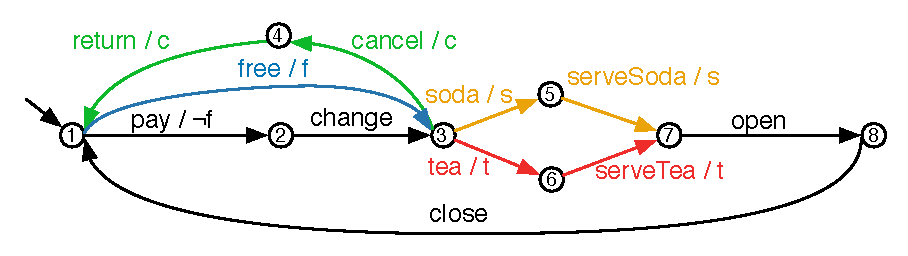
\includegraphics[width = 0.9\linewidth]{figures/fts.pdf}
	\caption{The FTS modeling the vending machine SPL}
	\label{fig:fts-vendingmachine}
\end{figure}

As an illustrative example, Figure~\ref{fig:fts-vendingmachine} depicts an FTS modeling of a product line of vending machines. In addition to an action, a transition in FTS is also labeled with an expression, called \emph{feature expression}, which defines the set of products able to enable this transition. For instance, the transition from state 3 to state 6 is labeled with the feature expression $t$, meaning that it can be executed only by products including the corresponding feature $t$. The transition from state 1 to state 2 is labeled with $\lnot f$, and thus can be executed only by products that do not have the feature $f$. More generally, the expression can be any formula that represents a subset of  products. The transition system representing the behavior  of a particular product is obtained by removing all transitions not available to this product. This operation is named \emph{projection}~\cite{Classen2013}.

Most of FTS-based analyses rely on the annotative model to design efficient CTL and LTL verification algorithms~\cite{Classen2013,Classen2014,Cordy2014}. The result %of these algorithms 
is a feature expression representing all the products that satisfy the property under verification. This feature expression can be represented in different ways. One representation sees a feature expression as two sets of features~\cite{Classen2010}: a set includes the features required to satisfy the property; the other contains the features that must be excluded. Alternatively, feature expressions can be represented as Boolean formulae where included (resp. excluded) features appear as positive (resp. negative) literals~\cite{Classen2013} (as done in Figure~\ref{fig:fts-vendingmachine}). The result of a given verification analysis is another feature expression, produced by computing conjunctions and disjunctions of the individual expressions.

Figure \ref{fig:fts-strategies} illustrates such variability-aware analysis of FTS, where the resulting feature expression is denoted as a Boolean formula.
On the top right corner, an FTS models the behavior of the vending machine product line.
Let us assume that this FTS is checked against the property ``the machine can only \texttt{return} if \texttt{pay} occurred'', which is violated by any product having both free drinks ($f$) and cancel ($c$) features.
Also, we take as example a feature selection for the vending machine selling soda and tea without the free drinks and cancel features.
The family-based analysis step $\hat{\alpha}$ applied to the FTS yields the feature expression $\lnot (c \land f)$. Then, pursuing a family-product-based strategy, one can evaluate this formula under the feature valuation corresponding to the aforementioned product. Doing so would yield $True$, meaning that the product satisfies the property.
Alternatively, one could follow a product-based strategy by projecting the FTS onto the specific product ($\pi$), yielding the transition system shown on the top left corner.
Thus, a classical verification procedure $\alpha$ yields that the product indeed satisfies the property.

\begin{figure}[t]
	\centering
    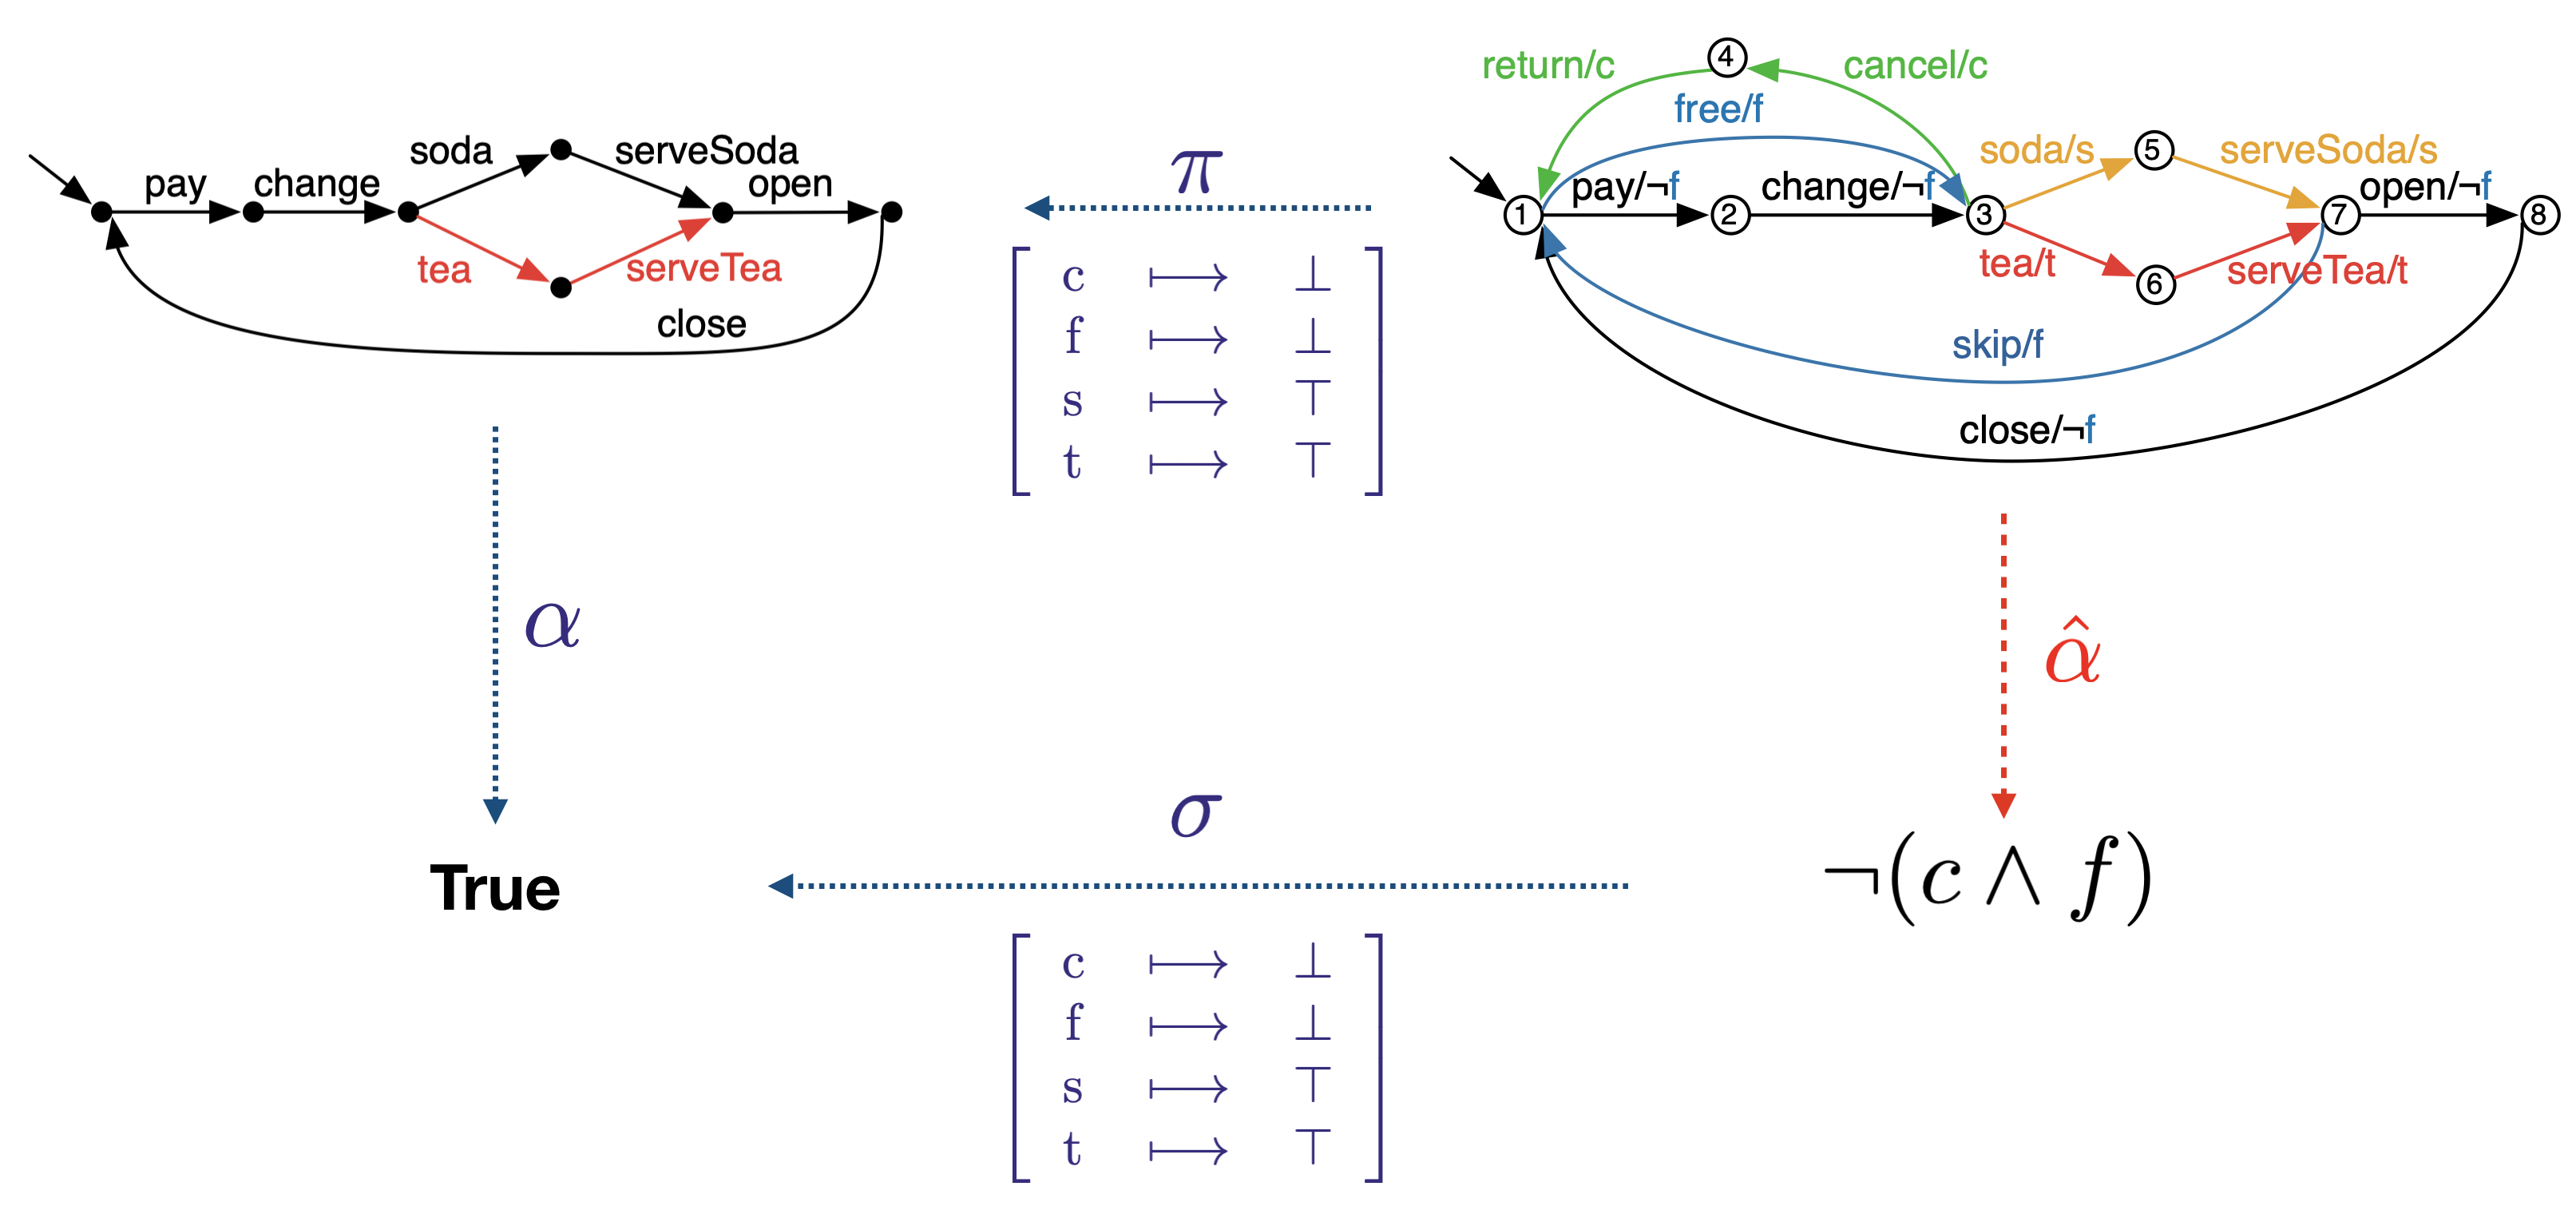
\includegraphics[width = 0.9\linewidth]{figures/fts-strategies.png}
	\caption{Product-based and family-product-based strategies applied to FTS verification}
	\label{fig:fts-strategies}
\end{figure}


Whatever representation one chooses for a feature expression, it can be concisely encoded in a Binary Decision Diagram (BDD)~\cite{Bryant1992,Classen2014}, similar to the ADD encoding of algebraic expressions in \Cref{fig:lifted-expression-example}.
The analysis of \citet{Classen2014} works fully symbolically: both the feature expressions and the state space are encoded as BDDs. The analysis proceeds classically, by induction on the structure of the CTL property, and by computing fixpoints backwards.
Differently, the analysis of \citet{Classen2013} is semi-symbolic: the state space of the model and the automaton of the property are represented explicitly, but the feature expressions are represented as BDDs. Model checking is performed forwards, as in SPIN \cite{Holzmann:2003}, but some states may be re-explored if they are reached with a new combination of features.

%Compositional reasoning on FTS has received less attention. Preliminary work~\cite{Cordy2012,Cordy2012d} studies the particular case where features only add or only remove behavior , and shows what properties are preserved upon the addition of these features. By applying this theory, one can thus infer the impact of each feature successively, and in the end determine which combinations of features lead to violations of the properties. Under the assumption that feature composition is commutative, BDD can again be used as an efficient encoding for these combinations. The general case where features have arbitrary impacts on the FTS remains to be addressed. Several papers deal with the compositional verification of features~\cite{Fisler2005,Liu2011}. Their application to FTS is a future work that is out of scope of this paper.

FTS is a formalism that falls into the category of \emph{annotative} models. Higher-level formalisms are also considered, namely fPromela \cite{Classen2013} (inspired by Promela \cite{Holzmann:2003}). Compositional models also exist. For example, Plath and Ryan~\cite{Plath2001} extended the SMV language to express how a feature modifies an SMV model, called fSMV. 
In fSMV, each feature is modeled in isolation, which paves the way for \emph{compositional} reasoning. \citet{Classen2014} showed that any fSMV model can be transformed into an FTS and vice versa, thereby proving that the compositional model is equivalent to the annotative one. This implies that any verification algorithm designed for one model also works on the other.

\begin{figure}[!htbp]
	\centering
	\begin{tikzpicture}[node distance=80pt and 100pt, align=center, text centered, on grid, scale=0.5]
	\fontsize{10}{12}
	\node (ts) {Transition\\System};
	\node [left= of ts] (fsmv) {SMV + fSMV};
	\node [right= of ts] (fts) {Featured\\Transition\\System};
	
	
	\node [below=of ts] (ctl-ltl) {CTL or LTL \\ (yes / no)};
%	\node [left= of ctl-ltl, below=of fsmv] (compExpr) {$\bot$};
	\node [right= of ctl-ltl, below=of fts] (famExpr) {Feature \\expression};
	
	
	\node [below=of ctl-ltl] (bdd) {BDD};
%	\node [left= of bdd, below=of compExpr] (compLift) {$\bot$};
	\node [right= of bdd, below=of famExpr] (famLift) {Lifted \\feature expression};
	
	\draw[product] (featModel) -- node [midway, above] {$\pi'$} (ts);
	\draw[product] (fts) -- node [midway, above] {$\pi$} (ts);
	\draw[family, <->] (featModel) to [bend left=25] node [midway, above] {$\gamma$} (famModel);
	
%	\draw[feature] (featModel) -- node [midway, left] {$\bot$} (featExpr);
	\draw[family] (fts) -- node [midway, right] {$\hat{\alpha}$} (famExpr);
	\draw[product] (ts) to node [midway, left] {$\alpha$} (ctl-ltl);
	
%	\draw[product] (featExpr) -- node [midway, above] {$\bot$} (reliability);
	\draw[product] (famExpr) -- node [midway, above] {$\sigma$} (ctl-ltl);
	%\draw[family] (featExpr) to [bend left=25] node [near end, above] {\hyperref[def:variability-encoding-function-expressions]{$\gamma$}} (famExpr);
	
%	\draw[family] (featExpr) -- node [midway, left] {$\bot$} (featLift);
	\draw[family] (famExpr) -- node [midway, right] {$\mathit{lift}$} (famLift);
	\draw[product] (bdd) to node [near start, left] {$\llbracket \_ \rrbracket_c$} (ctl-ltl);
	
%	\draw[family] (featLift) -- node [midway, above] {$\bot$} (bdd);
	\draw[family] (famLift) -- node [midway, above] {$\hat{\sigma}$} (bdd);
	
	\node [below= 25pt of bdd] (anchor) {};
	\node [left= 62pt of anchor.north, anchor=north west, draw=black, rounded corners=2pt, font=\scriptsize] (legend) {
		\settowidth{\columnLength}{FTS model checking checking}
		\begin{tabular}{ll|ll}
		$\pi$                    & projection \cite{Classen2013}  & $\pi'$ & feature composition~\cite{Plath2001} \\
		$\sigma$                     & product evaluation      & $\hat{\sigma}$  & BDD evaluation \\
		$\alpha$                     & model checking  & $\hat{\alpha}$  & FTS model checking~\cite{Classen2013,Classen2014} \\
		$\llbracket \_ \rrbracket_c$ & BDD application & $\gamma$ & lifted composition~\cite{Classen2014}\\
		$\mathit{lift}$ & maps expression into BDD semantics & \\ %$\bot$ & unexplored
		% & & $\delta$ & compositional reasoning
		\end{tabular}};
	\node [left= 10pt of legend.north west, anchor=north east, draw=black, rounded corners=2pt, font=\footnotesize] (legendStrat) {
		\begin{tabular}{ll}
		\raisebox{2pt}{\tikz{\draw[feature](0,0) -- (5mm,0);}} & feature-based\\
		\raisebox{2pt}{\tikz{\draw[family](0,0) -- (5mm,0);}} & family-based\\
		\raisebox{2pt}{\tikz{\draw[product](0,0) -- (5mm,0);}} & product-based
		\end{tabular}};
	\end{tikzpicture}
	\caption{Commutative diagram of product-line behavioral properties  verification strategies}
	\label{fig:diagram-FTS}
\end{figure}

\paragraph{Summary}
The above review of the state of the art of FTS verification suggests partial reuse of the structure of the commutative diagram in Figure~\ref{fig:strategies-overview}, resulting in Figure~\ref{fig:diagram-FTS}. From an FTS (see top right of Figure~\ref{fig:diagram-FTS}), one can pursue a product-based strategy by computing the projection ($\pi$) of each product and applying a standard model checking algorithm ($\alpha$). In contrast, family-based strategies start with the application of dedicated algorithms to FTS ($\hat{\alpha}$) to obtain the set of products satisfying the property. This set can either be enumerated ($\sigma$), giving rise to a family-product-based strategy, or lifted into a feature expression encoded in BDD semantics and then being evaluated without enumeration into a BDD ($\hat{\sigma}$).

On the other side, one finds the aforementioned fSMV model of Plath and Ryan~\cite{Plath2001}. The transition system of a particular product can be obtained by composing the base model with the model of each of its features ($\pi')$. A family-based approach can be followed to produce directly an FTS from the \emph{lifted composition}~\cite{Classen2014} of the base model and all the features ($\gamma$). Feature-based strategies have been proposed under specific assumptions (e.g., that features only add behavior) \cite{Cordy2012}, but do not apply outside such restricted scope. 
The soundness of the analyses is proved by the commutativity of the upper-right quadrant of Figure~\ref{fig:diagram-FTS} and by the equivalence result by~\citet{Classen2014}, similarly to Figure~\ref{fig:family-product-example}.

%\begin{figure}[!htbp]
%\centering
%\begin{tikzpicture}[node distance=80pt and 100pt, align=center, text centered, on grid, scale=0.5]
%    \fontsize{10}{12}
%    \node (dtmc) {DTMC};
%    \node [left= of dtmc, text width=70pt] (featModel) {\hyperref[def:feature-based-probabilistic-model]{Compositional model}};
%    \node [right= of dtmc, text width=70pt] (famModel) {\hyperref[def:150fdtmc]{Annotative model}};
%
%%    \node [below right=30pt and 50pt of featModel, text=gray] (featProdSound) {\footnotesize\Cref{theorem:feature-product-soundness}};
%%    \node [below left=30pt and 50pt of famModel, text=gray] (famProdSound) {\footnotesize\Cref{theorem:family-product-soundness}};
%%    \node [above=20pt of dtmc, text=gray] (varEnc) {\footnotesize\Cref{theorem:variability-encoding-soundness}};
%
%    \node [below=of dtmc] (reliability) {Reliability};
%    \node [left= of reliability, below=of featModel] (featExpr) {Compositional\\expressions};
%    \node [right= of reliability, below=of famModel] (famExpr) {Annotative\\expression};
%%    \node [above=20pt of reliability, text=gray] (varEncExpr) {\footnotesize\Cref{theorem:variability-encoding-expressions-soundness}};
%%
%%    \node [below right=40pt and 50pt of featExpr, text=gray] (featFamSound) {\footnotesize\Cref{theorem:feature-family-soundness}};
%%    \node [below left=40pt and 50pt of famExpr, text=gray] (famSound) {\footnotesize\Cref{theorem:family-soundness}};
%
%    \node [below=of reliability] (reliabilityADD) {Reliability\\ADD};
%    \node [left= of reliabilityADD, below=of featExpr] (featLift) {Compositional\\lifted expressions};
%    \node [right= of reliabilityADD, below=of famExpr] (famLift) {Annotative\\lifted expression};
%
%    \draw[product] (featModel) -- node [midway, above] {\hyperref[def:derivation-by-composition]{$\lambda'$}} (dtmc);
%    %\draw[product] (featModel) to [bend right=10] node [midway, below] {\hyperref[def:fdtmc-derivation]{$\lambda$}} (dtmc);
%    \draw[product] (famModel) -- node [midway, above] {\hyperref[def:fdtmc-derivation]{$\lambda$}} (dtmc);
%    \draw[family] (featModel) to [bend left=25] node [midway, above] {\hyperref[def:variability-encoding-function]{$\lambda_v$}} (famModel);
%
%    \draw[feature] (featModel) -- node [midway, left] {\hyperref[def:alpha_v]{$\alpha_v$}} (featExpr);
%    \draw[family] (famModel) -- node [midway, right] {\hyperref[def:alpha_v]{$\alpha_v$}} (famExpr);
%    \draw[product] (dtmc) to node [midway, left] {\hyperref[def:alpha]{$\alpha$}} (reliability);
%
%    \draw[product] (featExpr) -- node [midway, above] {\hyperref[def:sigma]{$\sigma$}} (reliability);
%    \draw[product] (famExpr) -- node [midway, above] {\hyperref[def:sigma]{$\sigma$}} (reliability);
%    \draw[family] (featExpr) to [bend left=25] node [near end, above] {\hyperref[def:variability-encoding-function-expressions]{$\lambda_v$}} (famExpr);
%
%    \draw[family] (featExpr) -- node [midway, left] {\hyperref[def:lift]{$\mathit{lift}$}} (featLift);
%    \draw[family] (famExpr) -- node [midway, right] {\hyperref[def:lift]{$\mathit{lift}$}} (famLift);
%    \draw[product] (reliabilityADD) to node [near start, left] {$\llbracket \_ \rrbracket_c$} (reliability);
%
%    \draw[family] (featLift) -- node [midway, above] {\hyperref[def:sigma_v]{$\sigma_v$}} (reliabilityADD);
%    \draw[family] (famLift) -- node [midway, above] {\hyperref[def:sigma_v]{$\sigma_v$}} (reliabilityADD);
%
%    \node [below= 25pt of reliabilityADD] (anchor) {};
%    \node [left= 62pt of anchor.north east, anchor=north west, draw=black, rounded corners=2pt, font=\scriptsize] (legend) {
%        \newlength{\columnLength}
%        \settowidth{\columnLength}{evaluation with ADDs}
%        \begin{tabular}{ll|ll}
%            $\lambda$                    & derivation      & $\lambda_v$ & variability encoding \\
%            $\sigma$                     & evaluation      & $\sigma_v$  & evaluation with ADDs \\
%            $\alpha$                     & model checking  & $\alpha_v$  & \multirow{2}{\columnLength}{parametric model checking} \\
%            $\llbracket \_ \rrbracket_c$ & ADD application &             &
%        \end{tabular}};
%    \node [left= 10pt of legend.north west, anchor=north east, draw=black, rounded corners=2pt, font=\footnotesize] (legendStrat) {
%        \begin{tabular}{ll}
%            \raisebox{2pt}{\tikz{\draw[feature](0,0) -- (5mm,0);}} & feature-based\\
%            \raisebox{2pt}{\tikz{\draw[family](0,0) -- (5mm,0);}} & family-based\\
%            \raisebox{2pt}{\tikz{\draw[product](0,0) -- (5mm,0);}} & product-based
%        \end{tabular}};
%\end{tikzpicture}
%\caption{Commutative diagram of product-line reliability analysis strategies}
%\label{fig:strategies-overview}
%\end{figure}

%In the remaining sections, we detail each of these strategies and analysis steps with the goal of making statements about their commuting relations.
%\Cref{sec:product} presents product-based analysis strategies for both annotative and compositional models, with the goal of establishing a baseline
%for the remaining soundness proofs.
%\Cref{sec:family-star} discusses family-product-based and family-based analyses of annotative models.
%Feature-product-based and feature-family-based analysis strategies are the subject of \Cref{sec:feature-star}, which focuses on compositional models.
%Finally, \Cref{sec:variability-encoding} bridges the gap between analyses of annotative and compositional models (function $\lambda_v$ in
%\Cref{fig:strategies-overview}), establishing their commutativity.
%
%
%\subsection{Product-based Strategies}
%\label{sec:product}
%
%Product-based analysis strategies are based on the analysis of generated products or models thereof~\cite{Thum2014}.
%In \Cref{sec:model-representations}, we have discussed how to represent probabilistic behavioral models of product lines as PMCs,
%using both annotative and compositional approaches.
%There, we also described how to derive models of individual products, both for the annotative and the compositional approaches.
%The generated models are plain DTMCs, that is, their variability has been resolved at derivation time.
%Thus, to analyze the generated models, one only needs to model-check the non-parametric probabilistic reachability for every such model.
%We hereafter denote this non-parametric model checking analysis step by the following function $\alpha$.
%
%\begin{definition}[Non-parametric model checking]
%\label{def:alpha}
%    The non-para\-met\-ric mod\-el checking step $\alpha: DTMC \to [0,1]$ consists of applying the algorithm by \citet{HahnHZ10}.
%    For a DTMC $\mathcal{D} =$ \dtmc{},
%    $$\alpha(\mathcal{D}) = Pr^{\mathcal{D}}(s_0, T)$$
%    Since a DTMC has no parameters, $\alpha$ yields constant functions, which we interpret as plain Real numbers.
%\end{definition}
%
%Although there are more efficient algorithms for reliability model checking of regular (non-parametric) DTMCs,
%we use the algorithm by \citet{HahnHZ10} in the above definition for uniformity, which eases understanding.
%Since this algorithm is sound (\Cref{lemma:pmc-soundness}), a working implementation of the presented theory is free
%to exploit another sound probabilistic reachability algorithm for performance reasons.
%
%Now we are able to define product-based analysis for annotative and compositional models.
%\begin{definition}[Product-based analysis of annotative models]
%\label{def:product-annotative}
%%References: def:150fdtmc, def:fdtmc-derivation, def:alpha
%    Given an annotative model \annotativeModel{}, a product-based analysis yields, for all $c \in \llbracket \mathit{FM} \rrbracket$,
%    $$\alpha(\lambda(\mathcal{P}, w, c))$$
%    or, alternatively,
%    $$\alpha(\llbracket \mathcal{P} \rrbracket^w_c)$$
%\end{definition}
%\begin{definition}[Product-based analysis of compositional models]
%\label{def:product-compositional}
%    Given a compositional model \compositionalModel{}, a product-based analysis yields, for all $c \in \llbracket \mathit{FM} \rrbracket$,
%    $$\alpha(\lambda'(\mathcal{P_\top}, w', c))$$
%    where $\mathcal{P_\top}$ is the maximal PMC in $\mathscr{P}$ under $\prec$.
%\end{definition}
%
%So, a product-based analysis results in a mapping from configurations to respective reliability values, such as
%$\{c \mapsto \alpha(\lambda(\mathcal{P}, w, c)) \;|\; c \in \llbracket \mathit{FM} \rrbracket\}$ for annotative models, for instance.
%%Nonetheless, we focus on the results for individual configurations both for simplicity and because it is sufficient to
%%make statements about commutativity with other strategies.
%
%\begin{framed}
%    Both analysis strategies presented in this \namecref{sec:product} derive models for individual products of a given
%    product line and then apply a single-product analysis technique as is.
%    Since single-product analyses represent the base case upon which product-line analyses are built, the product-based
%    strategies establish a baseline for proving the soundness of other strategies.
%\end{framed}
%
%
%\subsection{Family-based Strategies}
%\label{sec:family-star}
%
%According to \citet{Thum2014}, a family-based analysis strategy is one that (a) operates only on domain artifacts and
%that (b) incorporates the knowledge about valid feature combinations.
%In this \namecref{sec:family-star}, we explore this kind of strategy in the context of annotative probabilistic models,
%because they encode the behavior of all products of a product line in a single PMC.
%It is also possible to perform family-based analyses on a compositional model by first transforming it into an annotative
%one, but this is discussed later in \Cref{sec:variability-encoding}.
%
%First, we show how to perform an analysis that yields a reliability expression, which can in turn be evaluated
%for each valid configuration of the product line.
%This characterizes a family-product-based strategy (\Cref{sec:family-product}).
%Then, the aforementioned analysis is leveraged to build a pure family-based (i.e., non-enumerative) strategy (\Cref{sec:family}).
%At first, it may seem counterintuitive to present the family-product-based approach before the family-based one.
%However, we shall see that our pure family-based approach builds upon concepts of the hybrid family-product-based approach, and that
%performing one or the other is a matter of choosing product-based or family-based analysis steps after a preliminary family-based step.
%
%\subsubsection{Family-product-based Strategy}
%\label{sec:family-product}
%
%A family-product-based strategy is a family-based strategy followed by a prod\-uct-based strategy over intermediate results~\cite{Thum2014}.
%%After defining the mechanics of the specific family-product-based strategy described in this section, we prove its correctness by comparing it
%%to perfoming a naïve product-based strategy (i.e., generate every product and analyze each of them separately).
%The preliminary family-based step of our family-product-based analysis consists of applying parametric model checking of probabilistic
%reachability (\Cref{sec:probabilistic-reachability}) of the underlying PMC of the annotative model.
%This step is abstracted as a function $\alpha_v$, where the subscript $v$ denotes that it is a variability-aware version of the non-parametric
%model checking function $\alpha$ (\Cref{def:alpha}).
%\begin{definition}[Parametric model checking]
%\label{def:alpha_v}
%    The parametric model checking analysis step $\alpha_v: PMC_X \to \mathcal{F}_X$ consists of applying the algorithm by
%    \citet{HahnHZ10} for probabilistic reachability, which yields a rational expression $\varepsilon \in \mathcal{F}_X$ for a PMC
%    with variables set $X$.
%    For a PMC $\mathcal{P} =$ \pmc{}, the input target states of the algorithm are the ones in $T$.
%\end{definition}
%
%After performing parametric model checking, the result of reachability analysis is an expression over the same variables as the
%annotative input PMC, denoting the PMC's reliability as a function of these variables.
%Hence, we expect this annotative reliability expression to be evaluated using the same evaluation functions that restricted the possible behaviors
%in the original model.
%This \emph{expression evaluation}, which can be seen as model derivation applied to expressions, is captured in function $\sigma$.
%\begin{definition}[Expression evaluation]
%\label{def:sigma}
%    Given an expression $\varepsilon$ over a set $X$ of variables, an evaluation factory $w$,
%    and a configuration $c \in \llbracket \mathit{FM} \rrbracket$,
%    we define the expression evaluation function in a similar fashion as DTMC derivation:
%    $$\sigma(\varepsilon, w, c) = \varepsilon[X/w(c)]$$
%    Likewise, we can use $\llbracket \varepsilon \rrbracket^w_c$ to denote $\sigma(\varepsilon, w, c)$.
%\end{definition}
%
%The function $\sigma$ is applied to the reliability expression for all valid configurations of the product line,
%yielding the final product-based step.
%The resulting family-product-based approach for the analysis of annotative models is then defined as follows.
%\begin{definition}[Family-product-based analysis]
%\label{def:family-product}
%%References: def:alpha_v, def:sigma, def:150fdtmc
%    Given an annotative model \annotativeModel{}, the family-product-based analysis yields, for all $c \in \llbracket \mathit{FM} \rrbracket$,
%    $$\sigma(\alpha_v(\mathcal{P}), w, c)$$
%    or, alternatively,
%    $$\llbracket \alpha_v(\mathcal{P}) \rrbracket^w_c$$
%\end{definition}
%
%\Cref{fig:family-product-example} illustrates the family-product-based strategy in contrast with the product-based one
%(\Cref{sec:product}), providing an intuition for why they commute.
%DTMC derivation $\lambda$ and expression evaluation $\sigma$ are both performed for a configuration $c$ such that $c \models p_x$.
%This way, $w(c)(x) = 1$ and the reliability is $0.9801$.
%If $c$ were such that $x$ was absent (i.e., $c \not \models p_x$), then the reliability would be $0.99$.
%
%\begin{figure}[!htbp]
%    \centering
%    \begin{tikzpicture}[node distance=20pt and 20pt,
%                        align=center,
%                        text centered]%, on grid]
%        \scriptsize
%        \node [draw, circle] (s0) {$s_0$};
%        \node [draw, circle, right= of s0] (s1) {$s_1$};
%        \node [draw, circle, right= of s1] (s2) {$s_2$};
%        \node [draw, circle, right= of s2] (ssuc) {$s_{\mathit{suc}}$};
%        \node [draw, circle, below= of ssuc] (serr) {$s_{\mathit{err}}$};
%
%        \draw[->] (s0) to node [midway, above] {$0.99$} (s1);
%        \draw[->] (s0) to [bend right=25] node [near start, right] {$0.01$} (serr);
%        \draw[->] (s1) to node [midway, above] {$\mathbf{x}$} (s2);
%        \draw[->] (s1) to [bend left=35] node [midway, above] {$\mathbf{1-x}$} (ssuc);
%        \draw[->] (s2) to node [midway, above] {$0.99$} (ssuc);
%        \draw[->] (s2) to [bend right=25] node [near start, right] (shortlab) {$0.01$} (serr);
%        \draw[->] (ssuc) to [loop right, in=30, out=330, looseness=4] node [midway, right] (ssuclab) {$1$} (ssuc);
%        \draw[->] (serr) to [loop right, in=30, out=330, looseness=4] node [midway, right] (serrlab) {$1$} (serr);
%
%        \node [draw=none, rectangle, fit=(s0) (ssuc) (serrlab) (serr) (shortlab)] (fdtmc) {};
%
%        \node [draw, circle, below= 80pt of s0] (ss0) {$s_0$};
%        \node [draw, circle, right= of ss0] (ss1) {$s_1$};
%        \node [draw, circle, right= of ss1] (ss2) {$s_2$};
%        \node [draw, circle, right= of ss2] (sssuc) {$s_{\mathit{suc}}$};
%        \node [draw, circle, below= of sssuc] (sserr) {$s_{\mathit{err}}$};
%
%        \draw[->] (ss0) to node [midway, above] {$0.99$} (ss1);
%        \draw[->] (ss0) to [bend right=25] node [near start, right] {$0.01$} (sserr);
%        \draw[NewEdge] (ss1) to node [midway, above] {$1$} (ss2);
%        \draw[RemovedEdge] (ss1) to [bend left=35] node [midway, above] (sshortlab) {$0$} (sssuc);
%        \draw[->] (ss2) to node [midway, above] {$0.99$} (sssuc);
%        \draw[->] (ss2) to [bend right=25] node [near start, right] {$0.01$} (sserr);
%        \draw[->] (sssuc) to [loop right, in=30, out=330, looseness=4] node [midway, right] (sssuclab) {$1$} (sssuc);
%        \draw[->] (sserr) to [loop right, in=30, out=330, looseness=4] node [midway, right] (sserrlab) {$1$} (sserr);
%
%        \node [draw=none, rectangle, fit=(ss0) (sssuc) (sserrlab) (sserr) (sshortlab)] (dtmc) {};
%
%        \normalsize
%        \node [right= 50pt of fdtmc] (expr) {$0.9801\cdot x + 0.99\cdot(1-x)$};
%        \node at (expr|-dtmc) (reliability) {$0.9801$};
%
%        \draw[product] (fdtmc) to node [midway, left] {\hyperref[def:fdtmc-derivation]{$\lambda$}} (dtmc);
%        \draw[family] (fdtmc) to node [midway, above] {\hyperref[def:alpha_v]{$\alpha_v$}} (expr);
%        \draw[product] (dtmc) to node [midway, below] {\hyperref[def:alpha]{$\alpha$}} (reliability);
%        \draw[product] (expr) to node [midway, right] {\hyperref[def:sigma]{$\sigma$}} (reliability);
%    \end{tikzpicture}
%    \caption{
%        Example of family-product-based analysis ($\alpha_v$ followed by $\sigma$) in contrast to a
%        product-based analysis ($\lambda$ followed by $\alpha$) of an annotative PMC
%    }
%    \label{fig:family-product-example}
%\end{figure}
%
%To be considered sound, a family-product-based analysis must be equivalent to performing a product-based analysis of all products.
%This means that performing a parametric model checking step and then evaluating the resulting expression for each valid product
%must yield the same result as first deriving the original annotative model for each product and then performing non-parametric
%model checking on each resulting DTMC.
%To prove that this equivalence holds, we can leverage a more general result about PMCs and well-defined evaluations.
%
%\begin{lemma}[Commutativity of PMC and expression evaluations]
%\label{lemma:evaluations-commute}
%    Given any PMC $\mathcal{P} =$ \pmc{} and a well-defined evaluation $u$, it holds that
%    $$\alpha(\mathcal{P}[X/u]) = \alpha_v(\mathcal{P})[X/u]$$
%\end{lemma}
%\begin{proof}
%    \begin{align*}
%        \alpha(\mathcal{P}[X/u]) &= \alpha(\mathcal{P}_{u}) &\text{(syntax change)} \\
%                                 &= Pr^{\mathcal{P}_{u}}(s_0, T) &\text{(\Cref{def:alpha})} \\
%                                 \shortintertext{and, since $u$ is well-defined,}
%                                 &= \alpha_v(\mathcal{P})[X/u] &\text{(\Cref{lemma:pmc-soundness} and \Cref{def:alpha_v})}
%    \end{align*}
%\end{proof}
%
%Using this result, we are able to express the soundness of the family-product-based approach
%in the following \namecref{theorem:family-product-soundness}.
%
%\begin{theorem}[Soundness of family-product-based analysis]
%\label{theorem:family-product-soundness}
%%References: def:150fdtmc, def:family-product, def:alpha, def:sigma, def:alpha_v, def:product-annotative
%    Given an annotative model \annotativeModel{}, for all $c \in \llbracket \mathit{FM} \rrbracket$
%    $$\alpha(\llbracket \mathcal{P} \rrbracket^w_c) = \llbracket \alpha_v(\mathcal{P}) \rrbracket^w_c$$
%    Alternatively, $ \alpha(\lambda(\mathcal{P}, w, c)) = \sigma(\alpha_v(\mathcal{P}), w, c) $.
%\end{theorem}
%\begin{proof}
%    Since $w(c)$ is a well-defined evaluation (\Cref{lemma:150fdtmc-w-well-defined}), we can use it to instantiate
%    $u$ in \Cref{lemma:evaluations-commute}.
%    Thus, let $\mathcal{P} =$ \pmc{}.
%    \begin{align*}
%        \alpha(\llbracket \mathcal{P} \rrbracket^w_c) &= \alpha(\mathcal{P}[X/w(c)]) &\text{(\Cref{def:fdtmc-derivation})} \\
%                                                      &= \alpha_v(\mathcal{P})[X/w(c)] &\text{(\Cref{lemma:evaluations-commute,lemma:150fdtmc-w-well-defined})} \\
%                                                      &= \llbracket \alpha_v(\mathcal{P}) \rrbracket^w_c &\text{(\Cref{def:sigma})}
%    \end{align*}
%\end{proof}
%
%\begin{framed}
%    As a major result, \Cref{theorem:family-product-soundness} states that the diagram in \Cref{fig:family-product-soundness} commutes.
%    This diagram corresponds to the upper right quadrant in \Cref{fig:strategies-overview}.
%\end{framed}
%
%\begin{figure}[!htbp]
%    \centering
%    \begin{tikzpicture}[node distance=80pt and 100pt, align=center, text centered, on grid]
%        \fontsize{10}{12}
%        \node (dtmc) {DTMC};
%        \node [above=50pt of dtmc, text width=50pt] (famModel) {\hyperref[def:150fdtmc]{Annotative model}};
%
%        \node [right=of dtmc] (reliability) {Reliability};
%        \node [above=50pt of reliability, right=of famModel] (famExpr) {Annotative\\expression};
%
%        \draw[product] (famModel) -- node [midway, left] {\hyperref[def:fdtmc-derivation]{$\lambda$}} (dtmc);
%        \draw[family] (famModel) -- node [midway, above] {\hyperref[def:alpha_v]{$\alpha_v$}} (famExpr);
%        \draw[product] (dtmc) to node [midway, below] {\hyperref[def:alpha]{$\alpha$}} (reliability);
%        \draw[product] (famExpr) -- node [midway, right] {\hyperref[def:sigma]{$\sigma$}} (reliability);
%    \end{tikzpicture}
%    \caption{Statement of \Cref{theorem:family-product-soundness}}
%    \label{fig:family-product-soundness}
%\end{figure}
%
%\subsubsection{Family-based Strategy}
%\label{sec:family}
%
%The pure family-based strategy starts by applying parametric model checking to the given annotative model, as in the family-based step
%of the family-product-based strategy.
%However, instead of evaluating the resulting expression for each variant, we \emph{lift} it to an ADD-based reliability expression,
%which can be evaluated for all variants at once.
%While an expression is evaluated with real values, a lifted expression is evaluated using ADDs, which represent
%Boolean functions from features to real values.
%Each of these ADDs encode the values that a variable can assume according to each possible configuration, also known as
%\emph{variational data}~\cite{VariationalDataStructures}.
%Since this approach incorporates the knowledge of valid feature combinations, it is a family-based strategy.
%
%Let us take the vending machine product line (\Cref{fig:complete-annotative-vending-machine}) as an example.
%Its reliability expression after parametric model checking has 8 terms, one of which is $0.124659 \cdot t \cdot t_\mathit{taste}$.
%Starting from the evaluation factory $w$, we can derive functions $\psi_x$ that, for each variable $x$, take a configuration
%$c \in \llbracket \mathit{FM} \rrbracket$ as input and output the corresponding value $w(c)(x)$.
%For $t$ and $t_\mathit{taste}$, for instance, these functions would be as follows:
%\begin{align*}
%    \psi_t(      \mathtt{Tea}, \lnot \mathtt{Soda}, \lnot \mathtt{Taste}) &= 1   &\psi_{t_\mathit{taste}}(      \mathtt{Tea}, \lnot \mathtt{Soda}, \lnot \mathtt{Taste})  &= 0 \\
%    \psi_t(      \mathtt{Tea}, \lnot \mathtt{Soda},       \mathtt{Taste}) &= 1   &\psi_{t_\mathit{taste}}(      \mathtt{Tea}, \lnot \mathtt{Soda},       \mathtt{Taste})        &= 1 \\
%    \psi_t(\lnot \mathtt{Tea},       \mathtt{Soda}, \lnot \mathtt{Taste}) &= 0   &\psi_{t_\mathit{taste}}(\lnot \mathtt{Tea},       \mathtt{Soda}, \lnot \mathtt{Taste})  &= 0 \\
%    \psi_t(\lnot \mathtt{Tea},       \mathtt{Soda},       \mathtt{Taste}) &= 0   &\psi_{t_\mathit{taste}}(\lnot \mathtt{Tea},       \mathtt{Soda},       \mathtt{Taste})        &= 0
%\end{align*}
%Having each of these functions represented by an ADD enables the efficient computation of the reliability expression as another ADD $\hat{r}$,
%representing a Boolean function that could be defined pointwise as
%$\hat{r}(c) = 0.124659 \cdot \psi_t(c) \cdot \psi_{t_\mathit{taste}}(c)$
%(we omit the remaining terms for simplicity).
%
%We now formally define expression lifting, as well as the mechanics of generating ADD-based evaluations and evaluating lifted expressions.
%
%\begin{definition}[Expression lifting]
%\label{def:lift}
%    For a given rational expression $\varepsilon \in \mathcal{F}_X$, whose semantics is a rational function $\mathbb{R}^{|X|} \to \mathbb{R}$,
%    and a product line with $k$ features,
%    we define the lifted expression $\mathit{lift}(\varepsilon) = \hat{\varepsilon}$ as an expression which is syntactically equal
%    to $\varepsilon$, but whose semantics
%    is lifted to a rational function $(\mathbb{B}^k \to \mathbb{R})^{|X|} \to (\mathbb{B}^k \to \mathbb{R})$, such that:
%
%    \begin{itemize}
%        \item
%            The function's inputs are $k$-ary ADDs.
%        \item
%            Polynomial coefficients are interpreted as constant ADDs (e.g., the number $5$ becomes $c \in \mathbb{B}^k \mapsto 5$).
%            We denote a constant $a$ lifted to a constant ADD as $\hat{a}$, so that $\hat{a}(\bar{b}) = a$ (where $\bar{b}$ is a Boolean tuple).
%        \item
%            Arithmetic operators are lifted to their ADD-based counterparts.
%    \end{itemize}
%    Hence, the admitted evaluations for $\hat{\varepsilon}$ are of type $u: X \to (\mathbb{B}^k \to \mathbb{R})$,
%    so that variables are properly replaced by $k$-ary ADDs.
%\end{definition}
%
%By the above definition, lifted expressions are syntactically equal to their original (non-lifted) counterparts.
%However, instead of using Real arithmetics, we interpret operators, constants, and variables using ADDs and ADD arithmetics (\Cref{sec:ADD}).
%These semantically lifted expressions are sound in the sense that they denote functions that, when evaluated with a given configuration,
%yield the same results as if the variables of the original expressions would have been individually evaluated for the same configuration.
%
%\begin{lemma}[Soundness of expression lifting]
%\label{lemma:lifting-soundness}
%    If $\varepsilon$ is a rational expression over Real constants and variables $x_i \in X$,
%    $|X| = n$, $A_1,\dotsc,A_n$ are ADDs,
%    and $\hat{\varepsilon} = \mathit{lift}(\varepsilon)$, then
%    $$ \hat{\varepsilon}[x_1/A_1,\dotsc,x_n/A_n](\bar{b}) = \varepsilon[x_1/A_1(\bar{b}), \dotsc, x_n/A_n(\bar{b})] $$
%    where $\bar{b}$ is a vector of $k$ Booleans, corresponding to a selection of the $k$ features in a given product line.
%\end{lemma}
%\begin{proof}
%
%    The proof is by structural induction on expression $\varepsilon$.
%    The base cases are constant expressions and single variables:
%    \begin{itemize}
%        \item
%            $\varepsilon = c$, where $c \in \mathbb{R}$:
%
%            In this case, $\hat{\varepsilon} = \hat{c}$.
%            Since $\varepsilon$ has no variables (and neither has $\hat{\varepsilon}$), we apply the empty evaluation $[\;]$.
%            Thus, $\hat{\varepsilon}[\;](\bar{b}) = \hat{c}(\bar{b}) = c = \varepsilon = \varepsilon[\;]$.
%
%        \item
%            $\varepsilon = x$:
%
%            In this case, $\hat{\varepsilon} = x$.
%            If $A$ is an arbitrary ADD, then:
%            $\hat{\varepsilon}[x/A](\bar{b}) = A(\bar{b}) = \varepsilon[x/A(\bar{b})]$.
%    \end{itemize}
%
%    As induction hypothesis, for the expressions $\varepsilon = \varepsilon_1$ and $\varepsilon = \varepsilon_2$,
%    assume that the following holds:
%    \begin{equation*}
%        \tag{I.H.}
%        \hat{\varepsilon}[x_1/A_1,\dotsc,x_n/A_n](\bar{b}) = \varepsilon[x_1/A_1(\bar{b}), \dotsc, x_n/A_n(\bar{b})]
%    \end{equation*}
%    Let $u: X \to (\mathbb{B}^k \to \mathbb{R})$ be a lifted evaluation such that $u(x_i) = A_i$ is an ADD.
%    Since $\varepsilon$ is a rational expression (i.e., a quotient of polynomials, as yielded by a parametric model checking algorithm---see
%    \Cref{sec:pmc,sec:probabilistic-reachability}),
%    it involves only the four basic arithmetic operators and exponentiation to Natural powers.
%    Thus, we examine the cases where we perform ADD arithmetics (\Cref{sec:ADD}), corresponding to the allowed operations in $\varepsilon$:
%    \begin{itemize}
%        \item
%            $\varepsilon = \varepsilon_1 \odot \varepsilon_2$, where $\odot \in \{+, -, \times, \div\}$:
%
%            In this case, $\hat{\varepsilon} = \hat{\varepsilon_1} \odot \hat{\varepsilon_2}$.
%            Hence,
%            \begin{align*}
%                \hat{\varepsilon}[X/u](\bar{b}) &= \big( \hat{\varepsilon_1} \odot \hat{\varepsilon_2} \big)[X/u](\bar{b})      & \\
%                                                &= \big( \hat{\varepsilon_1}[X/u] \odot \hat{\varepsilon_2}[X/u] \big)(\bar{b}) & \text{(evaluation)} \\
%                                                &= \hat{\varepsilon_1}[X/u](\bar{b}) \odot \hat{\varepsilon_2}[X/u](\bar{b})    & \text{(ADD arithmetics)} \\
%                                                &= \hat{\varepsilon_1}[x_1/A_1,\dotsc,x_n/A_n](\bar{b}) & \\
%                                                & \qquad \odot \hat{\varepsilon_2}[x_1/A_1,\dotsc,x_n/A_n](\bar{b})    & \text{(expanding $u$)} \\
%                                                &= \varepsilon_1[x_1/A_1(\bar{b}),\dotsc,x_n/A_n(\bar{b})] & \\
%                                                & \qquad \odot \varepsilon_2[x_1/A_1(\bar{b}),\dotsc,x_n/A_n(\bar{b})]    & \text{(induction hypothesis)} \\
%                                                &= \big( \varepsilon_1 \odot \varepsilon_2 \big)[x_1/A_1(\bar{b}),\dotsc,x_n/A_n(\bar{b})]    & \text{(evaluation)} \\
%                                                &= \varepsilon[x_1/A_1(\bar{b}),\dotsc,x_n/A_n(\bar{b})]    &
%            \end{align*}
%
%        \item
%            $\varepsilon = \varepsilon_1^i$, where $i \in \mathbb{N}$:
%
%            In this case, $\hat{\varepsilon} = \hat{\varepsilon_1}^i$.
%            Hence,
%            \begin{align*}
%                \hat{\varepsilon}[X/u](\bar{b}) &= \hat{\varepsilon_1}^i[X/u](\bar{b})                          & \\
%                                                &= \hat{\varepsilon_1}[X/u]^i(\bar{b})                          & \text{(evaluation)} \\
%                                                &= \hat{\varepsilon_1}[X/u](\bar{b})^i                          & \text{(ADD arithmetics)} \\
%                                                &= \hat{\varepsilon_1}[x_1/A_1,\dotsc,x_n/A_n](\bar{b})^i       & \text{(expanding $u$)} \\
%                                                &= \varepsilon_1[x_1/A_1(\bar{b}),\dotsc,x_n/A_n(\bar{b})]^i    & \text{(induction hypothesis)} \\
%                                                &= \varepsilon_1^i[x_1/A_1(\bar{b}),\dotsc,x_n/A_n(\bar{b})]    & \text{(evaluation)} \\
%                                                &= \varepsilon[x_1/A_1(\bar{b}),\dotsc,x_n/A_n(\bar{b})]        &
%            \end{align*}
%    \end{itemize}
%
%%    Since $\varepsilon$ is an expression on $n$ variables, we can represent it without loss of generality
%%    as a quotient of two polynomials with $i$ and $j$ monomials each:
%%    $$\varepsilon = \frac{a_1x_1^{e_{1,1}} \dotsm x_n^{e_{1,n}} + \dotsb + a_ix_1^{e_{i,1}} \dotsm x_n^{e_{i,n}}}
%%                         {a'_1x_1^{e'_{1,1}} \dotsm x_n^{e'_{1,n}} + \dotsb + a'_jx_1^{e'_{j,1}} \dotsm x_n^{e'_{j,n}}}$$
%%
%%    Let $u: \mathbb{B}^k \to \mathbb{R}$ be a lifted evaluation such that $u(x_i) = A_i$ is an ADD.
%%    We have the following lifted expression after evaluating (with operators overloaded to denote ADD arithmetics):
%%\begin{align*}
%%    \hat{\varepsilon}[X/u] &= \hat{\varepsilon}[x_1/A_1,\dotsc,x_n/A_n] \\
%%                           &= \frac{\hat{a}_1A_1^{e_{1,1}} \dotsm A_n^{e_{1,n}} + \dotsb + \hat{a}_iA_1^{e_{i,1}} \dotsm A_n^{e_{i,n}}}
%%                                   {\hat{a}'_1A_1^{e'_{1,1}} \dotsm A_n^{e'_{1,n}} + \dotsb + \hat{a}'_jA_1^{e'_{j,1}} \dotsm A_n^{e'_{j,n}}}
%%\end{align*}
%%
%%Hence, using ADD arithmetics as defined in \Cref{sec:ADD},
%%\begin{align*}
%%    \hat{\varepsilon}[X/u](\bar{b}) &= \frac{\hat{a}_1A_1^{e_{1,1}} \dotsm A_n^{e_{1,n}} + \dotsb + \hat{a}_iA_1^{e_{i,1}} \dotsm A_n^{e_{i,n}}}
%%                                 {\hat{a}'_1A_1^{e'_{1,1}} \dotsm A_n^{e'_{1,n}} + \dotsb + \hat{a}'_jA_1^{e'_{j,1}} \dotsm A_n^{e'_{j,n}}}(\bar{b}) \\
%%                                 &= \frac{(\hat{a}_1A_1^{e_{1,1}} \dotsm A_n^{e_{1,n}} + \dotsb + \hat{a}_iA_1^{e_{i,1}} \dotsm A_n^{e_{i,n}})(\bar{b})}
%%                                 {(\hat{a}'_1A_1^{e'_{1,1}} \dotsm A_n^{e'_{1,n}} + \dotsb + \hat{a}'_jA_1^{e'_{j,1}} \dotsm A_n^{e'_{j,n}})(\bar{b})} \\
%%                                 &= \frac{(\hat{a}_1A_1^{e_{1,1}} \dotsm A_n^{e_{1,n}})(\bar{b}) + \dotsb + (\hat{a}_iA_1^{e_{i,1}} \dotsm A_n^{e_{i,n}})(\bar{b})}
%%                                 {(\hat{a}'_1A_1^{e'_{1,1}} \dotsm A_n^{e'_{1,n}})(\bar{b}) + \dotsb + (\hat{a}'_jA_1^{e'_{j,1}} \dotsm A_n^{e'_{j,n}})(\bar{b})} \\
%%                                 &= \frac{\hat{a}_1(\bar{b})A_1^{e_{1,1}}(\bar{b}) \dotsm A_n^{e_{1,n}}(\bar{b}) + \dotsb + \hat{a}_i(\bar{b})A_1^{e_{i,1}}(\bar{b}) \dotsm A_n^{e_{i,n}}(\bar{b})}
%%                                 {\hat{a}'_1(\bar{b})A_1^{e'_{1,1}}(\bar{b}) \dotsm A_n^{e'_{1,n}}(\bar{b}) + \dotsb + \hat{a}'_j(\bar{b})A_1^{e'_{j,1}}(\bar{b}) \dotsm A_n^{e'_{j,n}}(\bar{b})} \\
%%                                 &= \frac{a_1A_1(\bar{b})^{e_{1,1}} \dotsm A_n(\bar{b})^{e_{1,n}} + \dotsb + a_iA_1(\bar{b})^{e_{i,1}} \dotsm A_n(\bar{b})^{e_{i,n}}}
%%                                 {a'_1A_1(\bar{b})^{e'_{1,1}} \dotsm A_n(\bar{b})^{e'_{1,n}} + \dotsb + a'_jA_1(\bar{b})^{e'_{j,1}} \dotsm A_n(\bar{b})^{e'_{j,n}}} \\
%%                                 &= \varepsilon[x_1/A_1(\bar{b}), \dotsc, x_n/A_n(\bar{b})]
%%\end{align*}
%\end{proof}
%
%Note how a lifted expression demands a different type of evaluation, namely one that replaces variables with ADDs.
%To handle this interdependency, we correspondingly lift the evaluation factory.
%\begin{definition}[Lifted evaluation factory]
%\label{def:lifted-w}
%    Given an evaluation factory $w$ defined over a feature model $\mathit{FM}$ and a set $X$ of variables, the factory's lifted counterpart
%    is a function $\hat{w}: X \to (\mathbb{B}^{|\mathit{FM}|} \to \mathbb{R})$ that yields an ADD for a given variable.
%    This function is such that, for every variable $x \in X$ and all $c \in \llbracket \mathit{FM} \rrbracket$,
%    $$\hat{w}(x)(c) = w(c)(x)$$
%\end{definition}
%
%With a lifted evaluation factory, one can evaluate a lifted expression over the same set $X$ in a variability-aware fashion.
%The intuition is that we valuate each variable with an ADD that encodes all the real values it may assume for any configuration of the product line.
%\begin{definition}[Variability-aware expression evaluation]
%\label{def:sigma_v}
%    Let $\hat{w}$ be a lifted evaluation factory and $\hat{\varepsilon}$ be a lifted expression.
%    The variability-aware expression evaluation function, $\sigma_v$, is defined as
%    $$\sigma_v(\hat{\varepsilon}, \hat{w}) = \hat{\varepsilon}[X/\hat{w}]$$
%\end{definition}
%
%\begin{remark}
%\label{remark:lifting-generality}
%This definition of variability-aware evaluation is not restricted to reliability analysis or to the specific
%definitions of probabilistic models presented in this text.
%Indeed, one can notice that it relies on the definitions of an expression with rational function semantics and of
%an evaluation factory with respect to a given feature model.
%\end{remark}
%Thus, we are able to prove the following \namecref{theorem:sigma_v-soundness},
%which applies to product line analysis strategies that are based on expression evaluation.
%
%\begin{theorem}[Soundness of variability-aware expression evaluation]
%\label{theorem:sigma_v-soundness}
%    If $\varepsilon$ is an expression and $w$ is an evaluation factory with respect to a feature model $\mathit{FM}$,
%    let $\hat{\varepsilon}$ and $\hat{w}$ be their respective lifted counterparts.
%    Then, for all $c \in \llbracket \mathit{FM} \rrbracket$,
%    $$\sigma_v(\hat{\varepsilon}, \hat{w})(c) = \sigma(\varepsilon, w, c)$$
%    In other words, $\hat{\varepsilon}[X/\hat{w}](c) = \varepsilon[X/w(c)]$.
%\end{theorem}
%\begin{proof}
%    Using $\hat{w}$ as a substitution,
%    $$\hat{\varepsilon}[X/\hat{w}] = \hat{\varepsilon}[x_1/\hat{w}(x_1), \dotsc, x_n/\hat{w}(x_n)]$$
%
%    Thus, for all $c \in \llbracket \mathit{FM} \rrbracket$,
%    \begin{align*}
%        \sigma_v(\hat{\varepsilon}, \hat{w})(c) &= \hat{\varepsilon}[X/\hat{w}](c)                                  & \text{(\Cref{def:sigma_v})} \\
%                                                &= \hat{\varepsilon}[x_1/\hat{w}(x_1), \dotsc, x_n/\hat{w}(x_n)](c) & \\
%                                                &= \varepsilon[x_1/\hat{w}(x_1)(c), \dotsc, x_n/\hat{w}(x_n)(c)]    & \text{(\Cref{lemma:lifting-soundness})} \\
%                                                &= \varepsilon[x_1/w(c)(x_1), \dotsc, x_n/w(c)(x_n)]                & \text{(\Cref{def:lifted-w})} \\
%                                                &= \varepsilon[X/w(c)]                                              & \\
%                                                &= \sigma(\varepsilon, w, c)                                        & \text{(\Cref{def:sigma})}
%    \end{align*}
%\end{proof}
%
%We have seen that, in a product line with feature model $\mathit{FM}$, the presence function $p$ denotes a presence
%condition $p_x$ as a Boolean function $p(x): \llbracket \mathit{FM} \rrbracket \to \mathbb{B}$.
%Since this can be alternatively expressed as $p(x): \mathbb{B}^{|\mathit{FM}|} \to \mathbb{B}$, the presence function can also be encoded by ADDs,
%denoted by $\hat{p}(x)$.
%We now resort to the pointwise definition of $w$ as $w(c)(x) = p(x)(c)$ (\Cref{remark:pointwise-w}),
%to define a lifted evaluation factory $\hat{w}$, for evaluating the lifted version of expressions resulting
%from parametric model checking of an annotative model.
%
%\begin{lemma}[Soundness of lifted annotative evaluation factory]
%\label{lemma:p_add-soundness}
%    % References: def:presence-function
%    Given an annotative model \annotativeModel{} and a function $\hat{p}: X \to (\mathbb{B}^{|\mathit{FM}|} \to \mathbb{B})$
%    that encodes presence conditions for variables as ADDs, then
%    $\hat{w} = \hat{p}$ is a lifted evaluation factory for $w$.
%\end{lemma}
%\begin{proof}
%    From \Cref{def:150fdtmc}, we have that
%    \begin{align*}
%        w(c)(x) = \begin{cases}
%            1 &\mbox{if} \; p(x)(c) = 1 \\
%            0 &\mbox{otherwise}
%        \end{cases}
%    \end{align*}
%    Thus, from \Cref{remark:pointwise-w}, $w(c)(x) = p(x)(c)$.
%    Also, $p(x)(c) = \hat{p}(x)(c)$ by definition, so $w(c)(x) = \hat{p}(x)(c)$.
%\end{proof}
%
%Recalling the vending machine example, the presence conditions for the variables $t$ and $t_\mathit{taste}$ are, respectively,
%$\mathtt{Tea}$ and $\mathtt{Tea} \land \mathtt{Taste}$.
%Then, the ADDs $\hat{p}(t)$ and $\hat{p}(t_\mathit{taste})$ are given by the \Cref{fig:tea-add,fig:tea-taste-add},
%where we use the notation presented in \Cref{sec:ADD}.
%If we evaluate a lifted version of the example expression $\varepsilon = 0.124659 \cdot t \cdot t_\mathit{taste} + 0.3439 \cdot t$
%(2 terms from the actual reliability expression for the vending machine annotative model in \Cref{fig:complete-annotative-vending-machine})
%with $\hat{p}$, the resulting ADD will be $\hat{r} = 0.124659 \cdot \hat{p}(t) \cdot \hat{p}(t_\mathit{taste}) + 0.3439 \cdot \hat{p}(t)$,
%as depicted in
%\Cref{fig:example-add-solving}.
%Hence, for a given configuration $c \in \llbracket \mathit{FM} \rrbracket$, if both \texttt{Tea} and \texttt{Taste} are present
%(i.e., $\hat{p}(t)(c) = 1$ and $\hat{p}(t_\mathit{taste})(c) = 1$), then $\hat{r}(c) = 0.124659 \cdot 1 \cdot 1 + 0.3439 \cdot 1 = 0.468559$;
%if only \texttt{Tea} is present, then $\hat{r}(c) = 0.124659 \cdot 1 \cdot 0 + 0.3439 \cdot 1 = 0.3439$;
%and if both \texttt{Tea} and \texttt{Taste} are absent, then $\hat{r}(c) = 0$.
%
%\begin{figure}[!htbp]
%    \centering
%    \begin{subfigure}[t]{0.35\textwidth}
%        \centering
%        \begin{tikzpicture}[node distance=30pt, align=center, text centered, on grid]
%            \fontsize{10}{12}
%            \node [draw, ellipse] (fdec) {$\mathtt{Tea}$};
%            \node [draw, rectangle, below right= of fdec] (zero) {$0$};
%            \node [draw, rectangle, below left= of fdec] (one) {$1$};
%
%            \draw[-, dashed] (fdec) -- (zero);
%            \draw[-] (fdec) -- (one);
%        \end{tikzpicture}
%        \caption{$\hat{p}(t)$}
%        \label{fig:tea-add}
%    \end{subfigure}
%    \begin{subfigure}[t]{0.35\textwidth}
%        \centering
%        \begin{tikzpicture}[node distance=30pt, align=center, text centered, on grid]
%            \fontsize{10}{12}
%            \node [draw, ellipse] (fdec) {$\mathtt{Tea}$};
%            \node [draw, ellipse, below left= of fdec] (gdec) {$\mathtt{Taste}$};
%            \node [draw, rectangle, below right= of gdec] (zero) {$0$};
%            \node [draw, rectangle, below left= of gdec] (one) {$1$};
%
%            \draw[-] (fdec) -- (gdec);
%            \draw[-, dashed] (fdec) to [bend left=25] (zero);
%            \draw[-, dashed] (gdec) -- (zero);
%            \draw[-] (gdec) -- (one);
%        \end{tikzpicture}
%        \caption{$\hat{p}(t_\mathit{taste})$}
%        \label{fig:tea-taste-add}
%    \end{subfigure}
%    \begin{subfigure}[t]{\textwidth}
%        \centering
%        \begin{tikzpicture}[node distance=30pt, align=center, text centered, on grid]
%            \fontsize{10}{12}
%            \node [draw, ellipse] (sfdec) {$\mathtt{Tea}$};
%            \node [draw, ellipse, below left= of sfdec] (sgdec) {$\mathtt{Taste}$};
%            \node [draw, rectangle, below right= of sgdec] (sonlyt) {$0.3439$};
%            \node [draw, rectangle, below left= of sgdec] (sttaste) {$0.468559$};
%            \node [draw, rectangle, right= of sonlyt] (szero) {$0$};
%
%            \draw[-] (sfdec) -- (sgdec);
%            \draw[-, dashed] (sfdec) to [bend left=25] (szero);
%            \draw[-, dashed] (sgdec) -- (sonlyt);
%            \draw[-] (sgdec) -- (sttaste);
%        \end{tikzpicture}
%        \caption{$\mathit{lift}(0.124659 \cdot t \cdot t_\mathit{taste} + 0.3439 \cdot t)[t/\hat{p}(t), t_\mathit{taste}/\hat{p}(t_\mathit{taste})]$}
%        \label{fig:example-add-solving}
%    \end{subfigure}
%    \caption{Example of lifted expression evaluation using $\hat{p}$}
%    \label{fig:example-expression-solving}
%\end{figure}
%
%Using the result from \Cref{lemma:p_add-soundness}, we can now express the soundness of this family-based analysis step of evaluating lifted expressions.
%
%\begin{theorem}[Soundness of expression evaluation using $\hat{p}$]
%\label{theorem:add-encoding-soundness}
%    Given an annotative model \annotativeModel{},
%    $\varepsilon = \alpha_v(\mathcal{P})$, and $\hat{\varepsilon} = \mathit{lift}(\varepsilon)$,
%    let $\hat{p}$ be the encoding of the presence condition function $p$ to yield ADDs.
%    If we use $\hat{p}$ as a lifted evaluation factory, then for all $c \in \llbracket \mathit{FM} \rrbracket$
%    $$\llbracket \sigma_v(\hat{\varepsilon}, \hat{p}) \rrbracket_c = \llbracket \varepsilon \rrbracket^w_c$$
%
%    Alternatively, $ \sigma_v(\mathit{lift}(\varepsilon), \hat{p})(c) = \sigma(\varepsilon, w, c) $.
%\end{theorem}
%\begin{proof}
%    For a given annotative model, \Cref{lemma:p_add-soundness} states that $\hat{p}$ is a sound lifted counterpart of $w$.
%    Hence, by \Cref{theorem:sigma_v-soundness}, $\varepsilon[X/w(c)] = \hat{\varepsilon}[X/\hat{p}](c)$.
%    In other words, $\llbracket \sigma_v(\hat{\varepsilon}, \hat{p}) \rrbracket_c = \llbracket \varepsilon \rrbracket^w_c$.
%\end{proof}
%
%\begin{framed}
%    \Cref{fig:add-encoding-soundness} illustrates the main result from \Cref{theorem:add-encoding-soundness}.
%    The depicted diagram, which corresponds to the lower right quadrant in \Cref{fig:strategies-overview},
%    is commutative because of this \namecref{theorem:add-encoding-soundness}.
%\end{framed}
%
%\begin{figure}[!htbp]
%    \centering
%    \begin{tikzpicture}[node distance=80pt and 100pt, align=center, text centered, on grid]
%        \fontsize{10}{12}
%        \node (famExpr) {Annotative\\expression};
%        \node [right=of famExpr] (reliability) {Reliability};
%        \node [below=50pt of reliability] (reliabilityADD) {Reliability\\ADD};
%        \node [left= of reliabilityADD, below=50pt of famExpr] (famLift) {Annotative\\lifted expression};
%
%        \draw[product] (famExpr) -- node [midway, above] {\hyperref[def:sigma]{$\sigma$}} (reliability);
%        \draw[family] (famExpr) -- node [midway, left] {\hyperref[def:lift]{$\mathit{lift}$}} (famLift);
%        \draw[product] (reliabilityADD) to node [midway, right] {$\llbracket \_ \rrbracket_c$} (reliability);
%        \draw[family] (famLift) -- node [midway, above] {\hyperref[def:sigma_v]{$\sigma_v$}} (reliabilityADD);
%    \end{tikzpicture}
%    \caption{Statement of \Cref{theorem:add-encoding-soundness}}
%    \label{fig:add-encoding-soundness}
%\end{figure}
%
%Now that we have all analysis steps needed, we can formally define the family-based strategy.
%\begin{definition}[Family-based analysis]
%\label{def:family}
%%References: def:150fdtmc, def:sigma_v, def:lift, def:alpha_v
%    Given an annotative model \annotativeModel{}, a family-based analysis yields, for all $c \in \llbracket \mathit{FM} \rrbracket$,
%    $$\sigma_v \big( \mathit{lift}(\alpha_v(\mathcal{P})), \hat{p} \big)(c)$$
%    or, alternatively,
%    $$\llbracket \sigma_v \big( \mathit{lift}(\alpha_v(\mathcal{P})), \hat{p} \big) \rrbracket_c$$
%\end{definition}
%
%This definition may seem also enumerative at first, but the result is, in fact, a Boolean function (encoded as an ADD).
%The function application to a given configuration is meant only as a comparison to the other strategies.
%Indeed, family-based analysis is sound if, and only if, it yields an ADD for which every valid configuration
%$c \in \llbracket \mathit{FM} \rrbracket$ results in the same probability as if the original annotative model
%had been subject to product-based analysis for the same configuration $c$.
%
%\begin{theorem}[Soundness of family-based analysis]
%\label{theorem:family-soundness}
%%References: def:150fdtmc, def:product-annotative, def:family
%    Given an annotative model \annotativeModel{}, for all $c \in \llbracket \mathit{FM} \rrbracket$ it holds that
%    $$ \llbracket \sigma_v \big( \mathit{lift}(\alpha_v(\mathcal{P})), \hat{p} \big) \rrbracket_c = \alpha(\llbracket \mathcal{P} \rrbracket^w_c) $$
%\end{theorem}
%\begin{proof}
%    Follows from the successive application of \nameCrefs{theorem:family-product-soundness}
%    \labelcref{theorem:add-encoding-soundness} and \labelcref{theorem:family-product-soundness}:
%
%\begin{align*}
%    \llbracket \sigma_v \big( \mathit{lift}(\alpha_v(\mathcal{P})), \hat{p} \big) \rrbracket_c &= \llbracket \alpha_v(\mathcal{P}) \rrbracket^w_c & \text{(\Cref{theorem:add-encoding-soundness})} \\
%                                                                                               &= \alpha(\llbracket \mathcal{P} \rrbracket^w_c) & \text{(\Cref{theorem:family-product-soundness})}
%\end{align*}
%\end{proof}
%
%\begin{framed}
%    As a key result, \Cref{theorem:family-soundness} states that the diagram in \Cref{fig:family-soundness} commutes.
%    This diagram corresponds to the right half of the one in \Cref{fig:strategies-overview}.
%\end{framed}
%
%\begin{figure}[!htbp]
%
%    \centering
%    \begin{tikzpicture}[node distance=80pt and 100pt, align=center, text centered, on grid]
%        \fontsize{10}{12}
%        \node (dtmc) {DTMC};
%        \node [above=50pt of dtmc, text width=50pt] (famModel) {\hyperref[def:150fdtmc]{Annotative model}};
%
%        \node [right=of dtmc] (reliability) {Reliability};
%        \node [above=50pt of reliability, right=of famModel] (famExpr) {Annotative\\expression};
%
%        \draw[product] (famModel) -- node [midway, left] {\hyperref[def:fdtmc-derivation]{$\lambda$}} (dtmc);
%        \draw[family] (famModel) -- node [midway, above] {\hyperref[def:alpha_v]{$\alpha_v$}} (famExpr);
%        \draw[product] (dtmc) to node [midway, below] {\hyperref[def:alpha]{$\alpha$}} (reliability);
%        \draw[product] (famExpr) -- node [midway, right] {\hyperref[def:sigma]{$\sigma$}} (reliability);
%
%        \node [below right=25pt and 50pt of famModel, text=gray] (famProdSound) {\Cref{theorem:family-product-soundness}};
%
%        \node [below right=25pt and 50pt of famExpr, text=gray] (famSound) {\Cref{theorem:add-encoding-soundness}};
%
%        \node [right=of reliability] (reliabilityADD) {Reliability\\ADD};
%        \node [above= of reliabilityADD, right=of famExpr] (famLift) {Annotative\\lifted expression};
%
%        \draw[family] (famExpr) -- node [midway, above] {\hyperref[def:lift]{$\mathit{lift}$}} (famLift);
%        \draw[product] (reliabilityADD) to node [midway, below] {$\llbracket \_ \rrbracket_c$} (reliability);
%        \draw[family] (famLift) -- node [midway, right] {\hyperref[def:sigma_v]{$\sigma_v$}} (reliabilityADD);
%    \end{tikzpicture}
%    \caption{Statement of \Cref{theorem:family-soundness}}
%    \label{fig:family-soundness}
%\end{figure}
%
%
%\subsection{Feature-based Strategies}
%\label{sec:feature-star}
%
%A feature-based analysis strategy is one that (a) operates only on domain artifacts and that (b) analyzes the artifacts belonging to each
%feature in isolation~\cite{Thum2014}.
%Compositional models describe modular behaviors that represent units of variability.
%A given PMC within a compositional model may represent the behavior associated with one or more features, or even model
%part of a given feature's behavior (in case of behavior scattering).
%In this sense, analyzing individual PMCs of a compositional model can be seen as analyzing features in isolation, which is why
%we use this kind of probabilistic model to discuss feature-based strategies.
%Moreover, since our focus is on reliability, which is highly influenced by feature interactions, we cannot use a pure
%feature-based strategy~\cite{Thum2014}.
%Thus, we concentrate on feature-product-based and feature-family-based analysis strategies.
%
%Similar to what happens with family-based strategies (\Cref{sec:family-star}), the feature-family-based approach builds upon concepts
%used by the fea\-ture-prod\-uct-based strategy, and performing one or the other is a matter of choosing product-based or family-based analysis steps
%after a preliminary feature-based step.
%Because of that, we first discuss the feature-product-based strategy (\Cref{sec:feature-product}), focusing on the feature-based step
%of applying parametric model checking to each compositional PMC to generate corresponding compositional expressions.
%These reliability expressions can be evaluated for every possible configuration, yielding a product-based step and giving rise to a
%feature-product-based strategy.
%Alternatively, we can lift each expression and evaluate them using ADDs, in a similar fashion to what we did for the
%family-based strategy (\Cref{sec:family}).
%This leads to an overall feature-family-based strategy, which we discuss in \Cref{sec:feature-family}.
%
%
%\subsubsection{Feature-product-based Strategy}
%\label{sec:feature-product}
%
%A product-line analysis strategy is feature-product-based
%(a) if it consists of a feature-based analysis followed by a product-based analysis and
%(b) if the analysis results of the feature-based analysis are used in the product-based analysis~\cite{Thum2014}.
%The preliminary feature-based analysis step consists of applying the parametric model checking function $\alpha_v$
%to each PMC in a compositional model, yielding corresponding reliability expressions.
%These resulting expressions preserve the dependency relation, since each of them is defined in terms of the same variables
%as its originating PMC and can be assigned the same identifier.
%
%As an example, the compositional model of the vending machine product line (\Cref{fig:complete-compositional-vending-machine})
%yields the following expressions after the feature-based analysis step:
%$\alpha_v(\mathcal{P}_\top) = 1 \cdot t \cdot s$,
%$\alpha_v(\mathcal{P}_t) = 0.6561 \cdot t_\mathit{taste}$,
%$\alpha_v(\mathcal{P}_s) = 0.729 \cdot s_\mathit{taste}$,
%$\alpha_v(\mathcal{P}_{t_\mathit{taste}}) = 0.81$, and
%$\alpha_v(\mathcal{P}_{s_\mathit{taste}}) = 0.81$.
%
%A bottom-up evaluation of variables can be applied for each valid configuration, giving rise to
%the product-based analysis step.
%This procedure consists of \emph{compositional expression evaluation}, that is, expression evaluation using a \emph{compositional evaluation factory}
%derived from the composition factory used for the corresponding PMCs.
%
%\begin{definition}[Compositional evaluation factory]
%\label{def:compositional-evaluation-factory}
%    Given a compositional mod\-el \compositionalModel, a compositional evaluation factory is defined as
%    an evaluation factory (\Cref{def:evaluation-factory}) $w: \llbracket \mathit{FM} \rrbracket \to (I \to \mathbb{R})$,
%    such that for all $c \in \llbracket \mathit{FM} \rrbracket$ and $x \in I$,
%    \begin{align*}
%        w(c)(x) = \begin{cases}
%            \sigma(\alpha_v(\mathcal{P}), w, c) &\mbox{if} \; p(x)(c) = 1 \\
%            1 &\mbox{otherwise}
%        \end{cases}
%    \end{align*}
%    where $\mathit{idt}(\mathcal{P}) = x$.
%    Alternatively, we can write
%    \begin{align*}
%        w(c)(x) = \begin{cases}
%            \llbracket \alpha_v(\mathcal{P}) \rrbracket^w_c &\mbox{if} \; p(x)(c) = 1 \\
%            1 &\mbox{otherwise}
%        \end{cases}
%    \end{align*}
%\end{definition}
%
%In other words, whereas a composition factory composes a recursively derived version of PMC $\mathcal{P}'$ into slots identified by
%a variable $x$ of a PMC $\mathcal{P}$, a compositional evaluation factory composes a recursively evaluated version of
%$\alpha_v(\mathcal{P}')$ in every occurrence of the variable $x$ in $\alpha_v(\mathcal{P})$.
%This recursion always terminates, because $\prec$ is a well-founded relation.
%
%\begin{lemma}[Compositional evaluation terminates]
%\label{lemma:compositional-evaluation-terminates}
%    For a compositional model \compositionalModel{}, for all configurations $c \in \llbracket \mathit{FM} \rrbracket$,
%    the compositional evaluation $w(c)$ terminates.
%\end{lemma}
%\begin{proof}
%    Let $idt^{-1}: I \to \mathscr{P}$ be the inverse function of $idt$.
%    To prove $w(c)$ terminates, we note that the arguments in recursive calls to $w(c)$ (\Cref{def:compositional-evaluation-factory})
%    strictly decrease if we use $idt^{-1}$ as a measure function into the well-founded set $\mathscr{P}$.
%
%    Indeed, without loss of generality, let $x = idt(\mathcal{P})$ for some $\mathcal{P} \in \mathscr{P}$
%    with variables set $X = \{x_1, \dotsc, x_k\}$.
%    By definition of $\sigma$, the right-hand side of $w(c)(x)$ evaluates to either $1$ or
%    $\alpha_v(\mathcal{P})[x_1/w(c)(x_1),\allowbreak \dotsc,\allowbreak x_k/w(c)(x_k)]$.
%    In the first case, it trivially terminates; in the second, the arguments to each recursive call are the variables
%    $x_i \in X$.
%    By definition, $x_i = idt(\mathcal{P}_i)$ for some $\mathcal{P}_i \in \mathscr{P}$ such that $\mathcal{P}_i \prec \mathcal{P}$.
%    Thus, $idt^{-1}(x_i) \prec idt^{-1}(x)$.
%    Since $\prec$ is well-founded, $w(c)$ terminates.
%\end{proof}
%
%We define the feature-product-based analysis of compositional models as a recursive evaluation of the expressions obtained
%from the feature-based step, using the compositional evaluation factory shown above.
%This recursion starts from the maximal PMC in the compositional model, traversing the dependency graph induced by $\prec$
%(\Cref{fig:dependency-relation-example}) in a depth-first fashion.
%
%For the vending machine product line (\Cref{fig:complete-compositional-vending-machine}), for instance,
%the computation for configuration $c = \{\mathtt{Tea}, \mathtt{Taste}\}$ would be as follows:
%Starting with $\alpha_v(\mathcal{P}_\top)$, we evaluate the presence conditions for its variables, $t$ and $s$.
%Since $p_s = \mathtt{Soda}$ is not satisfied, $s$ is evaluated to $1$, ending the computation for this branch.
%On the other hand, $p_t = \mathtt{Tea}$ is satisfied, so we step into this branch to compute $\alpha_v(\mathcal{P}_t)$ under $c$.
%The only variable in this expression, $t_\mathit{taste}$, has its presence condition satisfied by $c$, so we step further into this branch
%to compute $\alpha_v(\mathcal{P}_{t_\mathit{taste}})$ under $c$.
%Since this expression denotes a constant value, we return this value and the recursion terminates, yielding the following constant expression:
%$$ \llbracket \alpha_v(\mathcal{P}_\top) \rrbracket_c = 1 \cdot \underbrace{\bigl( 0.6561 \cdot
%    \overbrace{(0.81)}^{\llbracket \alpha_v(\mathcal{P}_{t_\mathit{taste}}) \rrbracket_c} \bigr)}_{\llbracket \alpha_v(\mathcal{P}_t) \rrbracket_c}
%    \cdot \underbrace{(1)}_{\llbracket \alpha_v(\mathcal{P}_s) \rrbracket_c} $$
%We generalize and formalize this procedure as follows.
%
%\begin{definition}[Feature-product-based analysis]
%\label{def:feature-product}
%%References: def:feature-based-probabilistic-model, def:alpha_v, def:sigma
%    Given a compositional model \compositionalModel{} and the compositional evaluation factory $w$, derived from the composition factory $w'$,
%    the feature-product-based analysis yields, for all $c \in \llbracket \mathit{FM} \rrbracket$,
%    $$\sigma(\alpha_v(\mathcal{P}_\top), w, c)$$
%    or, alternatively,
%    $$\llbracket \alpha_v(\mathcal{P}_\top) \rrbracket^w_c$$
%    where $\mathcal{P}_\top$ is the maximal PMC in $\mathscr{P}$ under the dependency relation $\prec$.
%\end{definition}
%
%
%To establish the soundness of the feature-product-based strategy, we need to compare it to the product-based strategy for
%compositional models.
%However, the latter relies on PMC composition, while the former is based on compositional evaluation of expressions.
%To bridge this gap, we need to prove a few facts regarding the equivalence of evaluation and composition of PMCs.
%In certain circumstances, the PMCs yielded by both transformations have the same reliability.
%To prove this, we first note that, as far as reliability analysis is concerned,
%composing a PMC $\mathcal{P}'$ into a slot of another PMC $\mathcal{P}$ is equivalent to
%evaluating the corresponding variable in $\mathcal{P}$ with the reliability expression of $\mathcal{P}'$
%(i.e., $\alpha_v(\mathcal{P}')$).
%Whenever two analysis strategies yield equal reliability values, we say they are \emph{\reliabilityEquivalent}.
%
%\begin{lemma}[\MakeUppercase{\reliabilityEquivalence} of total composition and evaluation]
%\label{lemma:equivalence-in-compositions}
%    Let $\mathcal{P},\allowbreak \mathcal{P}_1,\allowbreak \dotsc,\allowbreak \mathcal{P}_k$ be compositional parametric Markov chains,
%    and $X = \{x_1, \dotsc, x_k\}$ be $\mathcal{P}$'s set of variables.
%    Then,
%    $$\alpha_v(\mathcal{P}[x_1/\mathcal{P}_1,\dotsc,x_k/\mathcal{P}_k]) = \alpha_v(\mathcal{P}[x_1/\alpha_v(\mathcal{P}_1),\dotsc,x_k/\alpha_v(\mathcal{P}_k)])$$
%    where the equals sign denotes \emph{extensional} equality.
%    In other words, the two expressions (i.e., syntactic objects) are not necessarily equal in a syntactical sense,
%    but their corresponding rational functions (i.e., semantic objects) always yield equal values if given equal inputs.
%\end{lemma}
%\begin{proof}
%    The main argument for this proof is the case where $\mathcal{P}$ has only one variable, that is, $X = \{x\}$.
%    This way, we start by proving that
%    $\alpha_v(\mathcal{P}[x/\mathcal{P}']) = \alpha_v(\mathcal{P}[x/\alpha_v(\mathcal{P}')])$
%    for a given compositional PMC $\mathcal{P}' =$ \compPmcPrime{'}.
%    Then, we extend this to the general case where $\mathcal{P}$ has an
%    arbitrary number of variables.
%
%    A generic illustration of $\mathcal{P}$ and $\mathcal{P}'$ is given by \Cref{fig:pmc-partial-composition-p,fig:pmc-partial-composition-pprime},
%    respectively.
%    Let $\mathcal{P}_e = \mathcal{P}[x/\alpha_v(\mathcal{P}')]$ be the PMC resulting from evaluation, denoted by \compPmcSub{e},
%    and $\mathcal{P}_c = \mathcal{P}[x/\mathcal{P}']$ be the PMC obtained by composition, denoted by the tuple \compPmcSub{c}.
%    \Cref{fig:alpha-equivalence-proof-pe,fig:alpha-equivalence-proof-pc} represent these PMCs and serve as a visual aid to the proof.
%
%    \begin{figure}[!htb]
%        %\Large
%        \fontsize{14.4}{17.28}
%        \centering
%        \begin{subfigure}[t]{\textwidth}
%            \centering
%            \begin{dot2tex}[
%                        dot,
%                        options=-tmath --autosize,
%                        scale=0.6
%                    ]
%            Digraph pe {
%                rankdir=LR;
%                node [shape="circle"];
%
%                s0 [label="s_0"];
%                many0 [label="\dots", shape="none"];
%                slot0 [label="s_{x_0}"];
%                slotsuc [label="s_{x_{\mathit{suc}}}"];
%                sloterr [label="s_{x_{\mathit{err}}}"];
%                many1suc [label="\dots", shape="none"];
%                many1err [label="\dots", shape="none"];
%                ssuc [label="s_{\mathit{suc}}"];
%                serr [label="s_{\mathit{err}}"];
%
%                s0 -> many0;
%                many0 -> slot0;
%                slot0 -> slotsuc [label="\mathit{Pr}^{\mathcal{P}'}(s'_0,s'_{\mathit{suc}})"];
%                slot0 -> sloterr [label="1-\mathit{Pr}^{\mathcal{P}'}(s'_0,s'_{\mathit{suc}})"];
%                slotsuc -> many1suc;
%                sloterr -> many1err;
%                many1suc -> ssuc;
%                many1err -> serr;
%                ssuc -> ssuc [label="1"];
%                serr -> serr [label="1"];
%            }
%            \end{dot2tex}
%            \caption{$\mathcal{P}_e = \mathcal{P}[x/\alpha_v(\mathcal{P}')]$}
%            \label{fig:alpha-equivalence-proof-pe}
%        \end{subfigure}
%        \begin{subfigure}[t]{\textwidth}
%            \centering
%            \begin{dot2tex}[
%                        dot,
%                        options=-tmath --autosize,
%                        scale=0.6
%                    ]
%            Digraph pc {
%                rankdir=LR;
%                node [shape="circle"];
%
%                s0 [label="s_0"];
%                many0 [label="\dots", shape="none"];
%                slot0 [label="s_{x_0}"];
%                slotsuc [label="s_{x_{\mathit{suc}}}"];
%                sloterr [label="s_{x_{\mathit{err}}}"];
%                many1suc [label="\dots", shape="none"];
%                many1err [label="\dots", shape="none"];
%                ssuc [label="s_{\mathit{suc}}"];
%                serr [label="s_{\mathit{err}}"];
%
%                s0 -> many0;
%                many0 -> slot0;
%                slotsuc -> many1suc;
%                sloterr -> many1err;
%                many1suc -> ssuc;
%                many1err -> serr;
%                ssuc -> ssuc [label="1"];
%                serr -> serr [label="1"];
%
%                ps0 [label="s'_0"];
%                pmany0 [label="\dots", shape="none"];
%                pssuc [label="s'_{\mathit{suc}}"];
%                pserr [label="s'_{\mathit{err}}"];
%
%                ps0 -> pmany0;
%                pmany0 -> pssuc;
%                pmany0 -> pserr;
%
%                pssuc -> slotsuc [label="1", style="bold"];
%                pserr -> sloterr [label="1", style="bold"];
%                slot0 -> ps0 [label="1", style="bold"];
%            }
%            \end{dot2tex}
%            \caption{$\mathcal{P}_c = \mathcal{P}[x/\mathcal{P}']$}
%            \label{fig:alpha-equivalence-proof-pc}
%        \end{subfigure}
%        \begin{subfigure}{\textwidth}
%            \centering
%            \begin{dot2tex}[
%                        dot,
%                        options=-tmath --autosize,
%                        scale=0.6
%                    ]
%            Digraph pcpartial {
%                rankdir=LR;
%                node [shape="circle"];
%
%                s0 [label="s_0"];
%                many0 [label="\dots", shape="none"];
%                slot0 [label="s_{x_0}"];
%                slotsuc [label="s_{x_{\mathit{suc}}}"];
%                sloterr [label="s_{x_{\mathit{err}}}"];
%                many1suc [label="\dots", shape="none"];
%                many1err [label="\dots", shape="none"];
%                ssuc [label="s_{\mathit{suc}}"];
%                serr [label="s_{\mathit{err}}"];
%
%                s0 -> many0;
%                many0 -> slot0;
%                slotsuc -> many1suc;
%                sloterr -> many1err;
%                many1suc -> ssuc;
%                many1err -> serr;
%                ssuc -> ssuc [label="1"];
%                serr -> serr [label="1"];
%
%                ps0 [label="s'_0"];
%                pssuc [label="s'_{\mathit{suc}}"];
%                pserr [label="s'_{\mathit{err}}"];
%
%                ps0 -> pssuc [label="\mathit{Pr}^{\mathcal{P}'}(s'_0,s'_{\mathit{suc}})"];
%                ps0 -> pserr [label="\mathit{Pr}^{\mathcal{P}'}(s'_0,s'_{\mathit{err}})"];
%
%                pssuc -> slotsuc [label="1", style="bold"];
%                pserr -> sloterr [label="1", style="bold"];
%                slot0 -> ps0 [label="1", style="bold"];
%            }
%            \end{dot2tex}
%            \caption{$\mathcal{P}_c$ after eliminating states $s' \in S' \setminus \mathit{interface}(\mathcal{P}')$}
%            \label{fig:alpha-equivalence-proof-pc-partial}
%        \end{subfigure}
%        \begin{subfigure}{\textwidth}
%            \centering
%            \begin{dot2tex}[
%                        dot,
%                        options=-tmath --autosize,
%                        scale=0.6
%                    ]
%            Digraph pcpartial {
%                rankdir=LR;
%                node [shape="circle"];
%
%                s0 [label="s_0"];
%                many0 [label="\dots", shape="none"];
%                slot0 [label="s_{x_0}"];
%                slotsuc [label="s_{x_{\mathit{suc}}}"];
%                sloterr [label="s_{x_{\mathit{err}}}"];
%                many1suc [label="\dots", shape="none"];
%                many1err [label="\dots", shape="none"];
%                ssuc [label="s_{\mathit{suc}}"];
%                serr [label="s_{\mathit{err}}"];
%
%                s0 -> many0;
%                many0 -> slot0;
%                slotsuc -> many1suc;
%                sloterr -> many1err;
%                many1suc -> ssuc;
%                many1err -> serr;
%                ssuc -> ssuc [label="1"];
%                serr -> serr [label="1"];
%
%                slot0 -> slotsuc [label="\mathit{Pr}^{\mathcal{P}'}(s'_0,s'_{\mathit{suc}})"];
%                slot0 -> sloterr [label="\mathit{Pr}^{\mathcal{P}'}(s'_0,s'_{\mathit{err}})"];
%            }
%            \end{dot2tex}
%            \caption{$\mathcal{P}_c$ after eliminating all states $s' \in S'$}
%            \label{fig:alpha-equivalence-proof-pc-partial-normalized}
%        \end{subfigure}
%        \caption{Generic PMCs in \Cref{lemma:equivalence-in-compositions}}
%    \end{figure}
%
%    Since $\alpha_v$ computes the probabilistic reachability property, we base this proof on the algorithm by \citet{HahnHZ10}.
%    This algorithm consists of successive eliminations of states, with the transition probability matrix being updated at each step.
%    A useful property, which \begin{NoHyper}\citeauthor{HahnHZ10}\end{NoHyper} use to prove that the algorithm is sound,
%    is that the probability of reaching the target states in the input PMC is an invariant, that is,
%    it remains the same throughout elimination steps.
%
%    Let us apply the algorithm by \citet{HahnHZ10} to $\mathcal{P}_c$.
%    For brevity, we show the composition via a single slot.
%    In the case where more slots exist, the following argument can be applied sequentially to each slot and corresponding renaming of $\mathcal{P}'$.
%
%    Since the order in which states are eliminated is not fixed, we first eliminate states $s' \in S' \setminus \mathit{interface(\mathcal{P}')}$.
%    The intermediate PMC at this point is given by \Cref{fig:alpha-equivalence-proof-pc-partial}.
%    These eliminations are restricted to states in $S'$, because the only transitions in $\mathbf{P}_c$ between states in $S$ and states in $S'$
%    are the ones connecting interface and slot (by construction---see \Cref{def:pmc-composition}).
%
%    Now, we eliminate the interface states.
%    Performing a single step of the algorithm by \begin{NoHyper}\citeauthor{HahnHZ10}\end{NoHyper}, we eliminate $s'_0$ and update $\mathbf{P}_c$ so that
%    \begin{align*}
%        \mathbf{P}_c(s_{x_0}, s'_{\mathit{suc}}) &= \mathbf{P}_c(s_{x_0}, s'_{\mathit{suc}}) + \mathbf{P}_c(s_{x_0}, s'_0) \cdot \frac{1}{1 - \mathbf{P}_c(s'_0, s'_0)} \cdot \mathbf{P}_c(s'_0, s'_{\mathit{suc}}) \\
%                                                 &= 0 + 1 \cdot \frac{1}{1 - 0} \cdot \mathit{Pr}^{\mathcal{P}'}(s'_0,s'_{\mathit{suc}}) \\
%                                                 &= \mathit{Pr}^{\mathcal{P}'}(s'_0,s'_{\mathit{suc}})
%    \end{align*}
%    Similarly, $\mathbf{P}_c(s_{x_0}, s'_{\mathit{err}}) = \mathit{Pr}^{\mathcal{P}'}(s'_0,s'_{\mathit{err}})$.
%    Repeating these steps for $s'_{\mathit{suc}}$ and $s'_{\mathit{err}}$, $\mathbf{P}_c$ is updated to have
%    $\mathbf{P}_c(s_{x_0}, s_{x_{\mathit{suc}}}) = \mathit{Pr}^{\mathcal{P}'}(s'_0,s'_{\mathit{suc}})$
%    and $\mathbf{P}_c(s_{x_0}, s_{x_{\mathit{err}}}) = \mathit{Pr}^{\mathcal{P}'}(s'_0,s'_{\mathit{err}})$
%    (see \Cref{fig:alpha-equivalence-proof-pc-partial-normalized}).
%
%    At this stage, all states $s' \in S'$ have been eliminated, so that $S_c = S = S_e$.
%    Furthermore, for all $s_1,s_2 \in S \setminus \mathit{slotStates}^{\mathcal{P}}(x)$, the transition probability matrices are such that
%    $\mathbf{P}_c(s_1, s_2) = \mathbf{P}(s_1, s_2) = \mathbf{P}_e(s_1, s_2)$ (\Cref{def:pmc-composition}).
%    Thus, the only difference between $\mathcal{P}_c$ and $\mathcal{P}_e$ are the transitions for slot states:
%    $(s_{x_0}, s_{x_{\mathit{suc}}})$ and $(s_{x_0}, s_{x_{\mathit{err}}})$.
%
%    For the ``success'' slot, $\mathbf{P}_c(s_{x_0}, s_{x_{\mathit{suc}}}) = \mathit{Pr}^{\mathcal{P}'}(s'_0,s'_{\mathit{suc}})$,
%    which is \emph{syntactically} equal to $\mathbf{P}_e(s_{x_0}, s_{x_{\mathit{suc}}})$.
%    So, we must prove that the ``error'' transitions, $\mathbf{P}_c(s_{x_0}, s_{x_{\mathit{err}}})$ and $\mathbf{P}_e(s_{x_0}, s_{x_{\mathit{err}}})$,
%    are extensionally equal.
%    But $s'_{\mathit{suc}}$ and $s'_{\mathit{err}}$ are the only two bottom strongly connected components of the underlying digraph of $\mathcal{P}'$
%    (\Cref{def:compositional-pmc}).
%    Thus, by Theorem 10.27 of \citet{baier_principles_2008},
%    $\mathit{Pr}^{\mathcal{P}'_u}(s'_0,s'_{\mathit{suc}}) + \mathit{Pr}^{\mathcal{P}'_u}(s'_0,s'_{\mathit{err}}) = 1$,
%    where $\mathcal{P}'_u$ is the DTMC obtained by applying some well-defined evaluation $u$ to $\mathcal{P}'$.
%    Since the choice of $u$ is arbitrary, $\mathbf{P}_c(s_{x_0}, s_{x_{\mathit{err}}})$ is extensionally equal to
%    $\mathbf{P}_e(s_{x_0}, s_{x_{\mathit{err}}})$.
%
%    This means that, at the current point of application of the probabilistic reachability algorithm to $\mathcal{P}_c$, $\mathbf{P}_c = \mathbf{P}_e$.
%    $\mathcal{P}_e$ and the partially analyzed $\mathcal{P}_c$ have the same probability of reaching the target state $s_{\mathit{suc}}$.
%    Moreover, since the algorithm preserves this probability at each step, the probabilistic reachability in $\mathcal{P}_c$
%    is the same at this point as before the algorithm started, and will remain the same until the algorithm stops.
%    Hence, $\alpha_v(\mathcal{P}[x/\mathcal{P}']) = \alpha_v(\mathcal{P}[x/\alpha_v(\mathcal{P}')])$.
%
%    To extend this proof to the case where $\mathcal{P}$ has an arbitrary number of variables, we repeat the argument that
%    the choice of states for elimination is arbitrary.
%    Let us assume, as induction hypothesis, that the \namecref{lemma:equivalence-in-compositions} holds for a PMC with $n$ variables.
%    If $\mathcal{P}$ has $n+1$ variables, we apply the same reasoning as in the single-variable case for one of $\mathcal{P}$'s slots,
%    $(s_{x_{{n+1}_0}}, s_{x_{{n+1}_\mathit{suc}}}, s_{x_{{n+1}_\mathit{err}}})$.
%    After eliminating \emph{only} the states corresponding to a composition at the given slot, we have the following extensional equalities:
%    $\mathbf{P}_c(s_{x_{{n+1}_0}}, s_{x_{{n+1}_\mathit{suc}}}) = \mathbf{P}_e(s_{x_{{n+1}_0}}, s_{x_{{n+1}_\mathit{suc}}})$ and
%    $\mathbf{P}_c(s_{x_{{n+1}_0}}, s_{x_{{n+1}_\mathit{err}}}) = \mathbf{P}_e(s_{x_{{n+1}_0}}, s_{x_{{n+1}_\mathit{err}}})$.
%    Also, the resulting PMC $\mathbf{P}_c$ has $n$ remaining slots, one for each variable.
%    By the induction hypothesis, after eliminating the states corresponding to all compositions in $\mathbf{P}_c$, we have
%    that $\mathbf{P}_c$ and $\mathbf{P}_e$ are extensionally equal.
%    Hence,
%    $\alpha_v(\mathcal{P}[x_1/\mathcal{P}_1,\dotsc,x_{n+1}/\mathcal{P}_{n+1}]) = \alpha_v(\mathcal{P}[x_1/\alpha_v(\mathcal{P}_1),\dotsc,x_{n+1}/\alpha_v(\mathcal{P}_{n+1})])$.
%\end{proof}
%
%Furthermore, since a composition of only DTMCs into a PMC yields another DTMC, both parametric and non-parametric model checking of this resulting
%chain (which has no variability) produce the same result.
%
%\begin{corollary}[\MakeUppercase{\reliabilityEquivalence} for composition with DTMCs]
%\label{corollary:equivalence-in-compositions-dtmc}
%% References: lemma:equivalence-in-compositions
%    Let $\mathcal{P}$ be a compositional PMC, $\mathcal{P}_1,\allowbreak \dotsc,\allowbreak \mathcal{P}_k$ be DTMCs,
%    and $X = \{x_1, \dotsc, x_k\}$ be $\mathcal{P}$'s variables set.
%    Then,
%    $$\alpha(\mathcal{P}[x_1/\mathcal{P}_1,\dotsc,x_k/\mathcal{P}_k]) = \alpha(\mathcal{P}[x_1/\alpha(\mathcal{P}_1),\dotsc,x_k/\alpha(\mathcal{P}_k)])$$
%\end{corollary}
%
%Now we have the tools to prove that our feature-product-based analysis is sound.
%We state this result in the following \namecref{theorem:feature-product-soundness}.
%
%\begin{theorem}[Soundness of feature-product-based analysis]
%\label{theorem:feature-product-soundness}
%%References: def:feature-product, def:product-compositional, def:feature-based-probabilistic-model
%    Given a compositional model \compositionalModel{}, for all configurations $c \in \llbracket \mathit{FM} \rrbracket$, it holds that
%    $$\sigma(\alpha_v(\mathcal{P}), w, c) = \alpha(\lambda'(\mathcal{P}, w', c))$$
%    or, alternatively,
%    $$\llbracket \alpha_v(\mathcal{P}) \rrbracket^w_c = \alpha(\llbracket \mathcal{P} \rrbracket^{w'}_c)$$
%    where $\mathcal{P} \in \mathscr{P}$ and $w$ is the compositional evaluation factory (\Cref{def:compositional-evaluation-factory})
%    derived from the composition factory $w'$.
%\end{theorem}
%\begin{proof}
%    We use well-founded induction.
%    The base of the induction is when $\mathcal{P}$ is minimal with respect to $\prec$.
%    In this case, $X = \emptyset$, so $\lambda'(\mathcal{P}, w', c) = \mathcal{P}$,
%    that is, $\alpha(\lambda'(\mathcal{P}, w', c)) = \alpha(\mathcal{P})$.
%    Likewise, $\alpha_v(\mathcal{P}) = \alpha(\mathcal{P})$, so that
%    $\sigma(\alpha_v(\mathcal{P}), w, c) = \sigma(\alpha(\mathcal{P}), w, c) = \alpha(\mathcal{P})$.
%    Thus, for the base case, $\sigma(\alpha_v(\mathcal{P}), w, c) = \alpha(\lambda'(\mathcal{P}, w', c))$.
%
%    Our induction hypothesis is that $\sigma(\alpha_v(\mathcal{P}_i), w, c) = \alpha(\lambda'(\mathcal{P}_i, w', c))$
%    for all $\mathcal{P}_i \in \mathscr{P}$ such that $\mathcal{P}_i \prec \mathcal{P}$ and $x_i = \mathit{idt}(\mathcal{P}_i)$, $i \in \{1,\dotsc,k\}$.
%    Let $\mathcal{P} \in \mathscr{P}$ be such that $\mathcal{P}_i \prec \mathcal{P}$ for all $i$.
%    By \Cref{def:sigma}, we have:
%    $$\sigma(\alpha_v(\mathcal{P}), w, c) = \alpha_v(\mathcal{P})[x_1/w(c)(x_1),\dotsc,x_k/w(c)(x_k)]$$
%    For each $x_i$, from the definition of the compositional evaluation factory $w$ (\Cref{def:compositional-evaluation-factory}),
%    \begin{align*}
%        w(c)(x_i) &= \begin{cases}
%            \sigma(\alpha_v(\mathcal{P}_i), w, c) &\mbox{if} \; p(x_i)(c) = 1 \\
%            1 &\mbox{otherwise}
%        \end{cases} \\
%                  &= \begin{cases}
%            \alpha(\lambda'(\mathcal{P}_i, w', c)) &\text{if} \; p(x_i)(c) = 1 \quad\quad \text{(by induction hypothesis)} \\
%            1 &\text{otherwise}
%        \end{cases}
%    \end{align*}
%    But, from the definition of the composition factory $w'$ (\Cref{def:feature-based-probabilistic-model}),
%    \begin{align*}
%        w'(c)(x_i) &= \begin{cases}
%            \mathcal{P}_i[X_i/w'(c)] &\mbox{if} \; p(x_i)(c) = 1 \\
%            \widetilde{\mathcal{P}} &\mbox{otherwise}
%        \end{cases} \\
%                  &= \begin{cases}
%            \lambda'(\mathcal{P}_i, w', c)) &\text{if} \; p(x_i)(c) = 1 \quad\quad\quad \text{(\Cref{def:derivation-by-composition})} \\
%            \widetilde{\mathcal{P}} &\text{otherwise}
%        \end{cases} \\
%        \shortintertext{Applying $\alpha$ to both sides,}
%        \alpha(w'(c)(x_i)) &= \begin{cases}
%            \alpha(\lambda'(\mathcal{P}_i, w', c)) &\text{if} \; p(x_i)(c) = 1 \\
%            \alpha(\widetilde{\mathcal{P}}) &\text{otherwise}
%        \end{cases} \\
%        \shortintertext{and, since $\alpha(\widetilde{\mathcal{P}}) = 1$,}
%                  &= \begin{cases}
%            \alpha(\lambda'(\mathcal{P}_i, w', c)) &\text{if} \; p(x_i)(c) = 1 \\
%            1 &\text{otherwise}
%        \end{cases} \\
%                  &= w(c)(x_i)
%    \end{align*}
%
%    Thus, $w(c)(x_i) = \alpha(w'(c)(x_i))$ and we have the following:
%    \begin{align*}
%        \sigma(\alpha_v(\mathcal{P}), w, c) &= \alpha_v(\mathcal{P})[x_1/w(c)(x_1),\dotsc,x_k/w(c)(x_k)] &\!\!\\
%            &= \alpha_v(\mathcal{P})[x_1/\alpha(w'(c)(x_1)),\dotsc,x_k/\alpha(w'(c)(x_k))] &\!\!\\
%            &= \alpha(\mathcal{P}[x_1/\alpha(w'(c)(x_1)),\dotsc,x_k/\alpha(w'(c)(x_k))]) &\!\!\text{(\Cref{lemma:evaluations-commute})}\\
%            &= \alpha(\mathcal{P}[x_1/w'(c)(x_1),\dotsc,x_k/w'(c)(x_k)]) &\!\!\text{(\Cref{corollary:equivalence-in-compositions-dtmc})}\\
%            &= \alpha(\lambda'(\mathcal{P}, w', c)) &\!\!\text{(\Cref{def:derivation-by-composition})}
%    \end{align*}
%\end{proof}
%
%\begin{framed}
%    As a further major result, \Cref{theorem:feature-product-soundness} states the diagram in \Cref{fig:feature-product-soundness} commutes.
%    This diagram relates to the upper left quadrant in \Cref{fig:strategies-overview}.
%\end{framed}
%%Note that \Cref{fig:strategies-overview} presents two derivation functions ($\lambda$ and $\lambda'$),
%%but we have only established the result for $\lambda'$ so far.
%
%\begin{figure}[!htbp]
%    \centering
%    \begin{tikzpicture}[node distance=80pt and 100pt, align=center, text centered, on grid]
%        \fontsize{10}{12}
%        \node (dtmc) {DTMC};
%        \node [above=50pt of dtmc, text width=65pt] (featModel) {\hyperref[def:feature-based-probabilistic-model]{Compositional model}};
%        \node [right= of dtmc] (reliability) {Reliability};
%        \node [above=50pt of reliability, right= of featModel] (featExpr) {Compositional\\expressions};
%
%        \draw[product] (featModel) -- node [midway, left] {\hyperref[def:derivation-by-composition]{$\lambda'$}} (dtmc);
%        \draw[feature] (featModel) -- node [midway, above] {\hyperref[def:alpha_v]{$\alpha_v$}} (featExpr);
%        \draw[product] (dtmc) to node [midway, below] {\hyperref[def:alpha]{$\alpha$}} (reliability);
%        \draw[product] (featExpr) -- node [midway, right] {\hyperref[def:sigma]{$\sigma$}} (reliability);
%    \end{tikzpicture}
%    \caption{Statement of \Cref{theorem:feature-product-soundness}}
%    \label{fig:feature-product-soundness}
%\end{figure}
%
%\subsubsection{Feature-family-based Strategy}
%\label{sec:feature-family}
%
%Similar to the family-based strategy (\Cref{sec:family}), the feature-family-based strategy leverages ADDs to store and reason
%about variational data.
%Since the preceding feature-based analysis yields expressions over reliabilities, this variational data is made of Real values
%corresponding to the reliabilities of the products of a product line.
%Again, lifting expressions involves lifting the corresponding evaluation factory.
%In this process, the presence conditions are encoded in ADDs to represent the variability under feature selection.
%This encoding is achieved by the ADD operator $\mathtt{ITE}$ (\emph{if-then-else}).
%
%Let us revisit expression evaluation in the vending machine example (\Cref{fig:complete-compositional-vending-machine}).
%We have seen the expression for $t_\mathit{taste}$ is the constant $0.81$, so its lifted version is the constant ADD $\widehat{0.81}$
%(according to the notation introduced in \Cref{def:lift}).
%The expression for $t$, $\alpha_v(\mathcal{P}_t) = 0.6561\cdot t_\mathit{taste}$, has the variable $t_\mathit{taste}$.
%Thus, if the presence condition $p_{t_\mathit{taste}} = \mathtt{Tea} \land \mathtt{Taste}$ is satisfied, this variable
%must be evaluated to the constant value $0.81$, assuming the value $1$ otherwise.
%Thus, the lifted expression $\widehat{\alpha_v(\mathcal{P}_t)}$ is evaluated with an ADD encoding this choice, given by
%$\varphi(t_\mathit{taste}) = \mathtt{ITE}(\widehat{p}(t_\mathit{taste}), \widehat{0.81}, \widehat{1})$
%and depicted in \Cref{fig:example-add-phi-tea-taste}.
%The evaluated lifted expression $\widehat{\alpha_v(\mathcal{P}_t)}[t_\mathit{taste}/\varphi(t_\mathit{taste})]$ is the ADD product
%of the constant $\widehat{0.6561}$ and $\varphi(t_\mathit{taste})$, shown in \Cref{fig:example-add-tea-solved}.
%The procedure is repeated for every composition, so that the variable $t$ in the expression $\widehat{\alpha_v(\mathcal{P}_\top)}$
%would be replaced by the ADD in \Cref{fig:example-add-phi-tea}, which already encodes the combined presence conditions for $t$ and
%$t_\mathit{taste}$.
%
%\begin{figure}[!htbp]
%    \fontsize{10}{12}
%    \centering
%    \begin{subfigure}[t]{0.45\textwidth}
%        \centering
%        \begin{tikzpicture}[node distance=30pt, align=center, text centered, on grid]
%            \node [draw, ellipse] (sfdec) {$\mathtt{Tea}$};
%            \node [draw, ellipse, below left= of sfdec] (sgdec) {$\mathtt{Taste}$};
%            \node [draw, rectangle, below left= of sgdec] (sttaste) {$0.81$};
%            \node [draw, rectangle, below right= of sgdec] (szero) {$1$};
%
%            \draw[-] (sfdec) -- (sgdec);
%            \draw[-, dashed] (sfdec) to [bend left=25] (szero);
%            \draw[-, dashed] (sgdec) -- (szero);
%            \draw[-] (sgdec) -- (sttaste);
%        \end{tikzpicture}
%        \caption{$\varphi(t_\mathit{taste}) = \mathtt{ITE}(\widehat{p}(t_\mathit{taste}), \widehat{0.81}, \widehat{1})$}
%        \label{fig:example-add-phi-tea-taste}
%    \end{subfigure}
%    \begin{subfigure}[t]{0.45\textwidth}
%        \centering
%        \begin{tikzpicture}[node distance=30pt, align=center, text centered, on grid]
%            \node [draw, ellipse] (sfdec) {$\mathtt{Tea}$};
%            \node [draw, ellipse, below left= of sfdec] (sgdec) {$\mathtt{Taste}$};
%            \node [draw, rectangle, below left= of sgdec] (sttaste) {$0.531441$};
%            \node [draw, rectangle, below right= of sgdec] (szero) {$0.6561$};
%
%            \draw[-] (sfdec) -- (sgdec);
%            \draw[-, dashed] (sfdec) to [bend left=25] (szero);
%            \draw[-, dashed] (sgdec) -- (szero);
%            \draw[-] (sgdec) -- (sttaste);
%        \end{tikzpicture}
%        \caption{$\widehat{\alpha_v(\mathcal{P}_t)}[t_\mathit{taste}/\varphi(t_\mathit{taste})]$}
%        \label{fig:example-add-tea-solved}
%    \end{subfigure}
%    \begin{subfigure}[t]{0.45\textwidth}
%        \centering
%        \begin{tikzpicture}[node distance=30pt, align=center, text centered, on grid]
%            \node [draw, ellipse] (sfdec) {$\mathtt{Tea}$};
%            \node [draw, ellipse, below left= of sfdec] (sgdec) {$\mathtt{Taste}$};
%            \node [draw, rectangle, below right= of sgdec] (sonlyt) {$0.6561$};
%            \node [draw, rectangle, below left= of sgdec] (sttaste) {$0.531441$};
%            \node [draw, rectangle, right= of sonlyt] (szero) {$1$};
%
%            \draw[-] (sfdec) -- (sgdec);
%            \draw[-, dashed] (sfdec) to [bend left=25] (szero);
%            \draw[-, dashed] (sgdec) -- (sonlyt);
%            \draw[-] (sgdec) -- (sttaste);
%        \end{tikzpicture}
%        \caption{$\varphi(t) = \mathtt{ITE}(\widehat{p}(t), \widehat{\alpha_v(\mathcal{P}_t)}, \widehat{1})$}
%        \label{fig:example-add-phi-tea}
%    \end{subfigure}
%    \caption{Example of lifted compositional expression evaluation}
%    \label{fig:example-feature-family-solving}
%\end{figure}
%
%The function $\varphi$ shown in the example is the lifted version of the compositional evaluation factory $w$.
%We first present a formal definition of $\varphi$ and then proceed to proving its soundness.
%Soundness of the feature-family-based strategy follows from this result and from the soundness of the
%feature-product-based strategy (\Cref{sec:feature-product}).
%
%\begin{definition}[Lifted compositional evaluation factory]
%\label{def:phi}
%    Given a compositional probabilistic model \compositionalModel{} and the compositional evaluation factory $w$, derived
%    from the composition factory $w'$, the lifted evaluation factory
%    $\varphi: I \to (\mathbb{B}^{|\mathit{FM}|} \to \mathbb{R})$ is a function that, for any $x \in I$, yields an ADD $\varphi(x)$ such that:
%    $$\varphi(x) = \mathtt{ITE}(\hat{p}(x), \widehat{\alpha_v(\mathcal{P})}[X/\varphi], \hat{\mathbf{1}})$$
%    where $\mathcal{P} \in \mathscr{P}$, $idt(\mathcal{P}) = x$, $\widehat{\alpha_v(\mathcal{P})} = \mathit{lift}(\alpha_v(\mathcal{P}))$
%    and $\hat{\mathbf{1}}$ is the constant ADD corresponding to the function $(c \in \llbracket \mathit{FM} \rrbracket) \mapsto 1$.
%\end{definition}
%
%The next \namecref{lemma:phi-encodes-w}, which is the compositional counterpart of \Cref{lemma:p_add-soundness},
%states this function $\varphi$ is indeed a lifted version of $w$.
%
%\begin{lemma}[Soundness of lifted compositional evaluation factory]
%\label{lemma:phi-encodes-w}
%    Given a compositional model \compositionalModel{} and the compositional evaluation factory $w$, derived
%    from the composition factory $w'$ (\Cref{def:compositional-evaluation-factory}),
%    for all $x \in I$ and all $c \in \llbracket \mathit{FM} \rrbracket$
%    it holds that $$\varphi(x)(c) = w(c)(x)$$
%\end{lemma}
%\begin{proof}
%    If $\mathcal{P} \in \mathscr{P}$ is such that $idt(\mathcal{P}) = x$, then
%    \begin{align*}
%        \varphi(x)(c) &= \mathtt{ITE}(\hat{p}(x), \widehat{\alpha_v(\mathcal{P})}[X/\varphi], \hat{\mathbf{1}})(c) \\
%                      &= \begin{cases}
%                          \widehat{\alpha_v(\mathcal{P})}[X/\varphi](c) &\mbox{if} \; \hat{p}(x)(c) \neq 0 \\
%                          \hat{\mathbf{1}}(c) &\mbox{if} \; \hat{p}(x)(c) = 0
%                      \end{cases}
%    \end{align*}
%
%    By \Cref{lemma:lifting-soundness},
%    $\widehat{\alpha_v(\mathcal{P})}[X/\varphi](c) = \alpha_v(\mathcal{P})[x_1/\varphi(x_1)(c), \dotsc, x_k/\varphi(x_k)(c)]$.
%    Also, $\forall_{c \in \llbracket \mathit{FM} \rrbracket} \cdot \hat{\mathbf{1}}(c) = 1$.
%    Thus,
%    \begin{align}
%        \label{eq:expanded-phi}
%        \varphi(x)(c) &= \begin{cases}
%            \alpha_v(\mathcal{P})[x_1/\varphi(x_1)(c), \dotsc, x_k/\varphi(x_k)(c)] &\mbox{if} \; \hat{p}(x)(c) \neq 0 \\
%            1 &\mbox{if} \; \hat{p}(x)(c) = 0
%        \end{cases}
%    \end{align}
%    On the other hand, $w$ is defined (\Cref{def:compositional-evaluation-factory}) as
%    \begin{align*}
%        w(c)(x) = \begin{cases}
%            \llbracket \alpha_v(\mathcal{P}) \rrbracket^w_c &\mbox{if} \; p(x)(c) \neq 0 \\
%            1 &\mbox{if} \; p(x)(c) = 0
%        \end{cases}
%    \end{align*}
%    Expanding the definition of $\llbracket \alpha_v(\mathcal{P}) \rrbracket^w_c$, we have
%    \begin{align}
%        \label{eq:expanded-w}
%        w(c)(x) = \begin{cases}
%            \alpha_v(\mathcal{P})[x_1/w(c)(x_1), \dotsc, x_k/w(c)(x_k)] &\mbox{if} \; p(x)(c) \neq 0 \\
%            1 &\mbox{if} \; p(x)(c) = 0
%        \end{cases}
%    \end{align}
%
%    Since $\hat{p}(x)(c) = p(x)(c)$, we compare corresponding cases in the \Cref{eq:expanded-phi,eq:expanded-w}.
%    The cases in which $p(x)(c) = 0$ are trivially equal. Otherwise, we use well-founded induction.
%
%    The base of our induction are minimal PMCs.
%    A minimal PMC $\mathcal{P}$ has no variables ($X = \emptyset$), so $\alpha_v(\mathcal{P})[X/u] = \alpha(\mathcal{P})$ for any evaluation $u$.
%    Since $w(c)$ is an evaluation, and considering $\varphi(x)(c)$ takes a variable $x$ to a Real number (thus, also being an evaluation),
%    we have that $\widehat{\alpha_v(\mathcal{P})}[X/\varphi](c) = \alpha_v(\mathcal{P})[X/w(c)]$ in this case.
%    For non-minimal PMCs, assume, as induction hypothesis, that $\widehat{\alpha_v(\mathcal{P}_j)}[X_j/\varphi](c) = \alpha_v(\mathcal{P}_j)[X_j/w(c)]$
%    for all $\mathcal{P}_j \prec \mathcal{P}$, where $j \in \{1,\dotsc,k\}$.
%    Then, for any $x_j \in X$,
%    \begin{align}
%        \varphi(x_j)(c) &= \begin{cases}\label{eq:induction-phi}
%            \widehat{\alpha_v(\mathcal{P}_j)}[X_j/\varphi](c) &\mbox{if} \; \hat{p}(x_j)(c) \neq 0 \\
%            1 &\mbox{if} \; \hat{p}(x_j)(c) = 0
%        \end{cases} \\
%        w(c)(x_j) &= \begin{cases}\label{eq:induction-w}
%            \alpha_v(\mathcal{P}_j)[X_j/w(c)] &\mbox{if} \; p(x_j)(c) \neq 0 \\
%            1 &\mbox{if} \; p(x_j)(c) = 0
%        \end{cases}
%    \end{align}
%
%    However, the induction hypothesis implies the right-hand sides of the \Cref{eq:induction-phi,eq:induction-w} are equal.
%    Thus, $\varphi(x_j)(c) = w(c)(x_j)$ for all $x_j \in X$, which means
%    $$\alpha_v(\mathcal{P})[x_1/\varphi(x_1)(c), \dotsc, x_k/\varphi(x_k)(c)] = \alpha_v(\mathcal{P})[x_1/w(c)(x_1), \dotsc, x_k/w(c)(x_k)]$$
%    and, by well-founded induction, the cases where $p(x)(c) = 1$ in the \Cref{eq:expanded-phi,eq:expanded-w} are also equal.
%    Hence, $\varphi(x)(c) = w(c)(x)$.
%\end{proof}
%
%This way, the ADDs yielded by function $\varphi$ from \Cref{def:phi} correctly encode the variation in values
%returned by the compositional evaluation factory $w$.
%An immediate consequence is that the expressions resulting from the feature-based analysis step can, indeed,
%be lifted and then evaluated using $\varphi$, and this gives us the same results as the corresponding (i.e., for the same
%configurations) product-based evaluations.
%This is expressed by the following soundness \namecref{theorem:phi-soundness}.
%
%\begin{theorem}[Soundness of expression evaluation using $\varphi$]
%\label{theorem:phi-soundness}
%    Given a compositional probabilistic model \compositionalModel{},
%    the compositional evaluation factory $w$, derived from the composition factory $w'$, and $x \in I$, let
%    $\mathcal{P} =$ \compPmc{} be such that $idt(\mathcal{P}) = x$, $\mathcal{P} \in \mathscr{P}$.
%    If $\varepsilon = \alpha_v(\mathcal{P})$, $\hat{\varepsilon} = \mathit{lift}(\varepsilon)$,
%    and $\varphi$ is the lifted compositional evaluation factory obtained from $w$ (\Cref{def:phi}),
%    then, for all $c \in \llbracket \mathit{FM} \rrbracket$, it holds that
%    $$\hat{\varepsilon}[X/\varphi](c) = \varepsilon[X/w(c)]$$
%\end{theorem}
%\begin{proof}
%    For the given compositional probabilistic model, \Cref{lemma:phi-encodes-w} states $\varphi$ is a sound lifted counterpart of $w$.
%    Hence, by \Cref{theorem:sigma_v-soundness}, $\varepsilon[X/w(c)] = \hat{\varepsilon}[X/\varphi](c)$.
%    In other words, $\llbracket \sigma_v(\hat{\varepsilon}, \varphi) \rrbracket_c = \llbracket \varepsilon \rrbracket^w_c$.
%\end{proof}
%
%\begin{framed}
%    So, \Cref{theorem:phi-soundness} states the diagram in \Cref{fig:phi-soundness} commutes.
%    This diagram corresponds to the lower left quadrant in \Cref{fig:strategies-overview}.
%\end{framed}
%
%\begin{figure}[!htbp]
%    \centering
%    \begin{tikzpicture}[node distance=80pt and 100pt, align=center, text centered, on grid]
%        \fontsize{10}{12}
%        \node (featExpr) {Compositional\\expressions};
%        \node [right=of featExpr] (reliability) {Reliability};
%
%        \node [below=50pt of reliability] (reliabilityADD) {Reliability\\ADD};
%        \node [left= of reliabilityADD, below=50pt of featExpr] (featLift) {Compositional\\lifted expressions};
%
%        \draw[product] (featExpr) -- node [midway, above] {\hyperref[def:sigma]{$\sigma$}} (reliability);
%        \draw[family] (featExpr) -- node [midway, left] {\hyperref[def:lift]{$\mathit{lift}$}} (featLift);
%        \draw[product] (reliabilityADD) to node [midway, right] {$\llbracket - \rrbracket_c$} (reliability);
%        \draw[family] (featLift) -- node [midway, below] {\hyperref[def:sigma_v]{$\sigma_v$}} (reliabilityADD);
%    \end{tikzpicture}
%    \caption{Statement of \Cref{theorem:phi-soundness}}
%    \label{fig:phi-soundness}
%\end{figure}
%
%The feature-family-based analysis strategy leverages the preceding results to yield an ADD encoding
%all reliabilities for valid configurations of the product line.
%This process is formally defined as follows.
%
%\begin{definition}[Feature-family-based analysis]
%\label{def:feature-family}
%%References: def:lift, def:feature-based-probabilistic-model, def:alpha_v, def:sigma_v, def:phi
%    Given a compositional model \compositionalModel{} and the lifted compositional evaluation factory
%    $\varphi$, derived from $w'$,
%    the feature-family-based strategy yields, for all $c \in \llbracket \mathit{FM} \rrbracket$,
%    $$\sigma_v \bigl(\mathit{lift}(\alpha_v(\mathcal{P}_\top)), \varphi \bigr) (c)$$
%    or, alternatively,
%    $$\llbracket (\mathit{lift} \circ \alpha_v) (\mathcal{P}_\top) \rrbracket^{\varphi}_c$$
%    where $\mathcal{P}_\top$ is the maximal PMC in $\mathscr{P}$ under the dependency relation $\prec$.
%\end{definition}
%
%Similar to the family-based strategy, the feature-family-based strategy is sound if this ADD is such that applying it to every
%valid configuration $c \in \llbracket \mathit{FM} \rrbracket$ results in the same probability as if the original compositional
%model had been derived for $c$ and the resulting DTMC had been model-checked for probabilistic reachability
%(product-based strategy).
%The difference is that, in the feature-family-based case, this statement must hold for every PMC in the compositional model.
%
%\begin{theorem}[Soundness of feature-family-based analysis]
%\label{theorem:feature-family-soundness}
%%References: def:feature-family, def:product-compositional, def:feature-based-probabilistic-model
%    Given a compositional model \compositionalModel{} and the lifted compositional evaluation factory $\varphi$, derived from $w'$,
%    for every PMC $\mathcal{P} \in \mathscr{P}$
%    and for all configurations $c \in \llbracket \mathit{FM} \rrbracket$ it holds that
%    $$ \llbracket (\mathit{lift} \circ \alpha_v) (\mathcal{P}_\top) \rrbracket^{\varphi}_c = \alpha(\llbracket \mathcal{P} \rrbracket^{w'}_c) $$
%\end{theorem}
%\begin{proof}
%    Let $w$ be the compositional evaluation factory derived from the composition factory $w'$.
%    The proof follows from successive application of \Cref{theorem:phi-soundness,theorem:feature-product-soundness}:
%
%\begin{align*}
%    \llbracket (\mathit{lift} \circ \alpha_v) (\mathcal{P}_\top) \rrbracket^{\varphi}_c &= \llbracket \sigma_v \big( \mathit{lift} ( \alpha_v(\mathcal{P})), \varphi \big) \rrbracket_c & \text{(\Cref{def:feature-family})} \\
%                                                                                        &= \llbracket \alpha_v(\mathcal{P}) \rrbracket^w_c & \text{(\Cref{theorem:phi-soundness})} \\
%                                                                                        &= \alpha(\llbracket \mathcal{P} \rrbracket^{w'}_c) & \text{(\Cref{theorem:feature-product-soundness})}
%\end{align*}
%\end{proof}
%
%\begin{framed}
%    As a key result, \Cref{theorem:feature-family-soundness} states the diagram in \Cref{fig:feature-family-soundness} commutes.
%    This diagram corresponds to the left half of the one in \Cref{fig:strategies-overview}.
%\end{framed}
%
%\begin{figure}[!htbp]
%    \centering
%    \begin{tikzpicture}[node distance=80pt and 100pt, align=center, text centered, on grid]
%        \fontsize{10}{12}
%        \node (dtmc) {DTMC};
%        \node [above=50pt of dtmc, text width=65pt] (featModel) {\hyperref[def:feature-based-probabilistic-model]{Compositional model}};
%        \node [right= of dtmc] (reliability) {Reliability};
%        \node [above=50pt of reliability, right= of featModel] (featExpr) {Compositional\\expressions};
%        \node [below right=25pt and 50pt of featModel, text=gray] (featProdSound) {\Cref{theorem:feature-product-soundness}};
%
%        \draw[product] (featModel) -- node [midway, left] {\hyperref[def:fdtmc-derivation]{$\lambda$}} (dtmc);
%        \draw[feature] (featModel) -- node [midway, above] {\hyperref[def:alpha_v]{$\alpha_v$}} (featExpr);
%        \draw[product] (dtmc) to node [midway, below] {\hyperref[def:alpha]{$\alpha$}} (reliability);
%        \draw[product] (featExpr) -- node [midway, right] {\hyperref[def:sigma]{$\sigma$}} (reliability);
%
%        \node [right= of reliability] (reliabilityADD) {Reliability\\ADD};
%        \node [above=50pt of reliabilityADD, right= of featExpr] (featLift) {Compositional\\lifted expressions};
%        \node [below right=25pt and 50pt of featExpr, text=gray] (featFamSound) {\Cref{theorem:phi-soundness}};
%
%        \draw[family] (featExpr) -- node [midway, above] {\hyperref[def:lift]{$\mathit{lift}$}} (featLift);
%        \draw[product] (reliabilityADD) to node [midway, below] {$\llbracket - \rrbracket_c$} (reliability);
%        \draw[family] (featLift) -- node [midway, right] {\hyperref[def:sigma_v]{$\sigma_v$}} (reliabilityADD);
%    \end{tikzpicture}
%    \caption{Statement of \Cref{theorem:feature-family-soundness}}
%    \label{fig:feature-family-soundness}
%\end{figure}
%
%
%\subsection{Bridging Compositional and Annotative Models}
%\label{sec:variability-encoding}
%
%Thus far, we have discussed family-based analysis strategies applied to annotative models and feature-based
%analysis strategies applied to compositional models.
%We now present a technique to transform any composition-based model into an \reliabilityEquivalent{} annotation-based model.
%This ability may be useful in the case that the reliability analysis of a given product line is predictably more efficient if performed
%using a strategy suited for annotative models, such as our family-product-based and family-based approaches.
%This transformation of models resembles \emph{variability encoding} techniques, that is, the rewriting of compile-time variability
%as load-time or run-time variability~\cite{FOSPL,ConfigurationLifting,VonRhein2016,VariabilityEncoding}.
%
%Although the concepts of compilation and execution are not defined for Markov chains, variability encoding,
%as established in the literature, has the main goal of creating artifacts that can be analyzed by off-the-shelf tools.
%Correspondingly, we are able to transform a compositional model, which cannot be directly model-checked (because it is split into a number
%of PMCs), into an annotative model, which can be immediately issued to a parametric model checker.
%Thus, we address the transformation of compositional models into annotative ones in terms of two \emph{variability encoding functions}:
%one operating on PMCs (\Cref{sec:variability-encoding-pmcs}) and the other for handling expressions
%(\Cref{sec:variability-encoding-expressions}).
%
%\subsubsection{Variability Encoding of PMCs}
%\label{sec:variability-encoding-pmcs}
%
%In terms of Markov chains, variability encoding can be realized by turning compositional models into annotative ones.
%This means transforming both the underlying compositional PMCs and the composition factory $w'$ into a single
%annotative PMC with a corresponding evaluation factory.
%To accomplish this, we propose an \emph{if-then-else} operator for PMCs that switches between possible states with a Boolean variable.
%
%\begin{definition}[\texttt{ITE} operator for PMCs]
%\label{def:pmc-ite}
%    Given two compositional PMCs, $\mathcal{P} =$ \compPmc{} and $\mathcal{P}' =$ \compPmcPrime{'}, and a variable $x \notin X \cup X'$,
%    the \emph{if-then-else} operator for PMCs is defined as
%    $$\mathtt{ITE}(x, \mathcal{P}, \mathcal{P}') = \mathcal{P}''$$
%    where $\mathcal{P}'' =$ \compPmcPrime{''} is a compositional PMC such that:
%    \begin{itemize}
%        \item
%            $S'' = S \cup S' \cup \{s''_0, s''_{\mathit{suc}}, s''_{\mathit{err}}\}$
%        \item
%            The state $s''_0$ is the new initial one, $s''_{\mathit{suc}}$ is the new success state, and $s''_{\mathit{err}}$ is the new error state.
%        \item
%            $X'' = X \cup X' \cup \{x\}$
%        \item
%            $T'' = \{s''_{\mathit{suc}}\}$
%        \item
%            $\mathbf{P}''$ is such that:
%            \begin{itemize}
%                \item
%                    $\mathbf{P}''(s''_0, s_0) = x$
%                \item
%                    $\mathbf{P}''(s''_0, s'_0) = 1-x$
%                \item
%                    $\mathbf{P}''(s_{\mathit{suc}}, s''_{\mathit{suc}}) = \mathbf{P}''(s'_{\mathit{suc}}, s''_{\mathit{suc}}) = \mathbf{P}''(s''_{\mathit{suc}}, s''_{\mathit{suc}}) = 1$
%                \item
%                    $\mathbf{P}''(s_{\mathit{suc}}, s_{\mathit{suc}}) = \mathbf{P}''(s'_{\mathit{suc}}, s'_{\mathit{suc}}) = 0$
%                \item
%                    $\mathbf{P}''(s_{\mathit{err}}, s''_{\mathit{err}}) = \mathbf{P}''(s'_{\mathit{err}}, s''_{\mathit{err}}) = \mathbf{P}''(s''_{\mathit{err}}, s''_{\mathit{err}}) = 1$
%                \item
%                    $\mathbf{P}''(s_{\mathit{err}}, s_{\mathit{err}}) = \mathbf{P}''(s'_{\mathit{err}}, s'_{\mathit{err}}) = 0$
%                \item
%                    For all remaining combinations of $s_1, s_2 \in S''$:
%                    \begin{align*}
%                        \mathbf{P}''(s_1, s_2) = \begin{cases}
%                            \mathbf{P}(s_1, s_2)  &\mbox{if} \; s_1, s_2 \in S  \\
%                            \mathbf{P}'(s_1, s_2) &\mbox{if} \; s_1, s_2 \in S' \\
%                            0                     &\mbox{otherwise} \\
%                        \end{cases}
%                    \end{align*}
%            \end{itemize}
%    \end{itemize}
%\end{definition}
%
%\begin{figure}[!htb]
%    \Large
%    \centering
%    \begin{subfigure}[t]{0.3\textwidth}
%        \centering
%        \begin{dot2tex}[
%                    dot,
%                    options=-tmath --autosize,
%                    scale=0.5
%                ]
%        Digraph itep {
%            rankdir=LR;
%            node [shape="circle"];
%
%            s0 [label="s_0"];
%            many0 [label="\dots", shape="none"];
%            ssuc [label="s_{\mathit{suc}}"];
%            serr [label="s_{\mathit{err}}"];
%
%            s0 -> many0;
%            many0 -> ssuc;
%            many0 -> serr;
%            ssuc -> ssuc [label="1"];
%            serr -> serr [label="1"];
%        }
%        \end{dot2tex}
%        \caption{$\mathcal{P}$}
%        \label{fig:pmc-ite-p}
%    \end{subfigure}
%    \begin{subfigure}[t]{0.3\textwidth}
%        \centering
%        \begin{dot2tex}[
%                    dot,
%                    options=-tmath --autosize,
%                    scale=0.5
%                ]
%        Digraph itepp {
%            rankdir=LR;
%            node [shape="circle"];
%
%            ps0 [label="s'_0"];
%            pmany0 [label="\dots", shape="none"];
%            pssuc [label="s'_{\mathit{suc}}"];
%            pserr [label="s'_{\mathit{err}}"];
%
%            ps0 -> pmany0;
%            pmany0 -> pssuc;
%            pmany0 -> pserr;
%            pssuc -> pssuc [label="1"];
%            pserr -> pserr [label="1"];
%        }
%        \end{dot2tex}
%        \caption{$\mathcal{P'}$}
%        \label{fig:pmc-ite-pprime}
%    \end{subfigure}
%    \begin{subfigure}[b]{0.5\textwidth}
%        \centering
%        \begin{dot2tex}[
%                    dot,
%                    options=-tmath --autosize,
%                    scale=0.5
%                ]
%        Digraph pcomppp {
%            rankdir=LR;
%            node [shape="circle"];
%
%            pps0 [label="s''_0"];
%            ppssuc [label="s''_{\mathit{suc}}"];
%            ppserr [label="s''_{\mathit{err}}"];
%
%            s0 [label="s_0"];
%            many0 [label="\dots", shape="none"];
%            ssuc [label="s_{\mathit{suc}}"];
%            serr [label="s_{\mathit{err}}"];
%
%            s0 -> many0;
%            many0 -> ssuc;
%            many0 -> serr;
%            ssuc -> ssuc [label="1", color="RemovedEdgeColor", style="dashed"];
%            serr -> serr [label="1", color="RemovedEdgeColor", style="dashed"];
%
%            ps0 [label="s'_0"];
%            pmany0 [label="\dots", shape="none"];
%            pssuc [label="s'_{\mathit{suc}}"];
%            pserr [label="s'_{\mathit{err}}"];
%
%            ps0 -> pmany0;
%            pmany0 -> pssuc;
%            pmany0 -> pserr;
%            pssuc -> pssuc [label="1", color="RemovedEdgeColor", style="dashed"];
%            pserr -> pserr [label="1", color="RemovedEdgeColor", style="dashed"];
%
%            pps0 -> s0 [label="x", color="NewEdgeColor", style="bold"];
%            pps0 -> ps0 [label="1-x", color="NewEdgeColor", style="bold"];
%            ssuc -> ppssuc [label="1", color="NewEdgeColor", style="bold"];
%            serr -> ppserr [label="1", color="NewEdgeColor", style="bold"];
%            pssuc -> ppssuc [label="1", color="NewEdgeColor", style="bold"];
%            pserr -> ppserr [label="1", color="NewEdgeColor", style="bold"];
%            ppssuc -> ppssuc [label="1", color="NewEdgeColor", style="bold"];
%            ppserr -> ppserr [label="1", color="NewEdgeColor", style="bold"];
%        }
%        \end{dot2tex}
%        \caption{$\mathtt{ITE}(x,\mathcal{P},\mathcal{P}')$}
%        \label{fig:pmc-ite-p2prime}
%    \end{subfigure}
%    \caption{Example \texttt{ITE} operator for PMCs}
%    \label{fig:pmc-ite-example}
%\end{figure}
%
%\Cref{fig:pmc-ite-example} illustrates this \texttt{ITE} operation.
%Again, green bold arrows represent new transitions, whereas red dashed ones are removed.
%Intuitively, an evaluation that maps $x$ to 1 yields a PMC with the same behavior as $\mathcal{P}$ (consequent),
%while an evaluation that maps $x$ to 0 yields a PMC with the same behavior as $\mathcal{P}'$ (alternative).
%We formalize this behavioral switching in terms of \reliabilityEquivalence{}.
%
%\begin{lemma}[\MakeUppercase{\reliabilityEquivalence} for \texttt{ITE}]
%\label{lemma:alpha-equivalence-ite}
%    Given two compositional PMCs, $\mathcal{P} =$ \compPmc{} and $\mathcal{P}' =$ \compPmcPrime{'}, and a variable $x \notin X \cup X'$,
%    let $\mathcal{P}'' = \mathtt{ITE}(x, \mathcal{P}, \mathcal{P}')$.
%    If \annotativeModelFundamental{''} is an annotative model with $\mathcal{P}''$ as its underlying PMC\footnote{
%        By \Cref{def:compositional-pmc}, any compositional PMC is also an annotative PMC (\Cref{def:annotative-pmc}).
%        Thus, a compositional PMC can be the underlying PMC of an annotative model.
%    }, where $p$, $w$, and $\mathit{FM}$ are arbitrarily chosen, then, for every $c \in \llbracket \mathit{FM} \rrbracket$,
%    \begin{align*}
%        \alpha(\llbracket \mathtt{ITE}(x, \mathcal{P}, \mathcal{P}') \rrbracket^w_c) = \begin{cases}
%            \alpha(\llbracket \mathcal{P} \rrbracket^w_c) &\mbox{if} \; p(x)(c) = 1 \\
%            \alpha(\llbracket \mathcal{P}' \rrbracket^w_c) &\mbox{otherwise}
%        \end{cases}
%    \end{align*}
%\end{lemma}
%\begin{proof}
%    We are interested in computing the probability of reaching $s''_{\mathit{suc}}$ from $s''_0$ in
%    $\mathcal{P}'' = \mathtt{ITE}(x, \mathcal{P}, \mathcal{P}')$ under evaluation $w(c)$.
%    In $\mathcal{P}''$, $s''_0 \neq s''_{\mathit{suc}}$ and $s''_{\mathit{suc}}$ is reachable from $s''_0$
%    (since $s''_{\mathit{suc}}$ is, by definition, reachable from $s_{\mathit{suc}}$ and $s'_{\mathit{suc}}$).
%    Hence, the reachability of $s''_{\mathit{suc}}$ from $s''_0$ satisfies \Cref{def:dtmc-probabilistic-reachability},
%    by which the probability of reaching state $s_2$ from state $s_1$ in a DTMC $\mathcal{D} =$ \dtmc{} is given by
%    $$Pr^{\mathcal{D}}(s_1, s_2) = \sum_{s' \in S \setminus \{s_2\}}{\mathbf{P}(s_1, s') \cdot Pr^{\mathcal{D}}(s', s_2)} + \mathbf{P}(s_1, s_2)$$
%
%    By \Cref{def:pmc-ite}, $\mathbf{P}''(s''_0, s_0) = x$, $\mathbf{P}''(s''_0, s'_0) = 1-x$,
%    and $\mathbf{P}''(s''_0, s'') = 0$ for all other $s'' \in S''$.
%    Thus,
%    \begin{align*}
%        \alpha(\llbracket \mathcal{P}'' \rrbracket^w_c) &= Pr^{\mathcal{P}''_{w(c)}}(s''_0, s''_{\mathit{suc}}) \\
%                                                      &= \sum_{s'' \in S'' \setminus \{s''_{\mathit{suc}}\}}{\mathbf{P}''_{w(c)}(s''_0, s'') \cdot Pr^{\mathcal{P}''_{w(c)}}(s'', s''_{\mathit{suc}})} + \mathbf{P}''_{w(c)}(s''_0, s''_{\mathit{suc}}) \\
%                                                      &= \sum_{s'' \in S'' \setminus \{s''_{\mathit{suc}}\}}{\mathbf{P}''_{w(c)}(s''_0, s'') \cdot Pr^{\mathcal{P}''_{w(c)}}(s'', s''_{\mathit{suc}})} + 0 \\
%                                                      &= \mathbf{P}''_{w(c)}(s''_0, s_0) \cdot Pr^{\mathcal{P}''_{w(c)}}(s_0, s''_{\mathit{suc}}) + \mathbf{P}''_{w(c)}(s''_0, s'_0) \cdot Pr^{\mathcal{P}''_{w(c)}}(s'_0, s''_{\mathit{suc}}) \\
%                                                      &= w(c)(x) \cdot Pr^{\mathcal{P}''_{w(c)}}(s_0, s''_{\mathit{suc}}) + (1 - w(c)(x)) \cdot Pr^{\mathcal{P}''_{w(c)}}(s'_0, s''_{\mathit{suc}})
%    \end{align*}
%    Since $w(c)(x)$ equals 1 if $p(x)(c) = 1$ and 0 otherwise (\Cref{def:150fdtmc}),
%    \begin{align*}
%        \alpha(\llbracket \mathcal{P}'' \rrbracket^w_c) &= \begin{cases}
%            Pr^{\mathcal{P}''_{w(c)}}(s_0, s''_{\mathit{suc}}) &\mbox{if} \; p(x)(c) = 1 \\
%            Pr^{\mathcal{P}''_{w(c)}}(s'_0, s''_{\mathit{suc}}) &\mbox{otherwise}
%        \end{cases}
%    \end{align*}
%
%    But, since $s_0 \in S$ and the only state in $S$ that can reach $s''_{\mathit{suc}}$ is $s_{\mathit{suc}}$
%    (\Cref{def:pmc-ite}), the probability of reaching $s''_{\mathit{suc}}$ from $s_0$ is the probability of reaching
%    $s_{\mathit{suc}}$ from $s_0$ multiplied by the transition probability from $s_{\mathit{suc}}$ to $s''_{\mathit{suc}}$:
%    \begin{align*}
%        Pr^{\mathcal{P}''_{w(c)}}(s_0, s''_{\mathit{suc}}) &= Pr^{\mathcal{P}''_{w(c)}}(s_0, s_{\mathit{suc}}) \cdot \mathbf{P}''_{w(c)}(s_{\mathit{suc}}, s''_{\mathit{suc}}) \\
%                                                           &= Pr^{\mathcal{P}_{w(c)}}(s_0, s_{\mathit{suc}}) \cdot 1 \\
%                                                           &= Pr^{\mathcal{P}_{w(c)}}(s_0, s_{\mathit{suc}}) \\
%                                                           &= \alpha(\llbracket \mathcal{P} \rrbracket^w_c)
%    \end{align*}
%
%    Similar reasoning applied to $S'$ leads to $Pr^{\mathcal{P}''_{w(c)}}(s'_0, s''_{\mathit{suc}}) = \alpha(\llbracket \mathcal{P}' \rrbracket_c)$.
%    Hence,
%    \begin{align*}
%        \alpha(\llbracket \mathcal{P}'' \rrbracket^w_c) &= \begin{cases}
%            \alpha(\llbracket \mathcal{P} \rrbracket^w_c) &\mbox{if} \; p(x)(c) = 1 \\
%            \alpha(\llbracket \mathcal{P}' \rrbracket^w_c) &\mbox{otherwise}
%        \end{cases}
%    \end{align*}
%\end{proof}
%
%The above \namecref{lemma:alpha-equivalence-ite} establishes the \texttt{ITE} operator has the effect of alternating behaviors
%if the resulting PMC is evaluated by replacing the switching variable $x$ with $0$ or $1$.
%However, the PMC operands of \texttt{ITE} are part of a compositional model, so their own variables are interpreted as placeholders to be used
%during composition (see \Cref{sec:compositional-models}), instead.
%To cope with this mismatch, we only use the \texttt{ITE} operator with PMCs that are either plain DTMCs or that result themselves
%from variability encoding.
%
%Hence, we define the variability encoding of PMCs as a composition of PMCs using the \texttt{ITE} operator in a recursive way,
%with minimal PMCs as the base case.
%The alternative choice (second argument to \texttt{ITE}) is always the trivial PMC $\widetilde{\mathcal{P}}$ (\Cref{def:trivial-pmc}),
%meaning no probabilistic behavior is actually added if the presence condition is not satisfied.
%This is coherent with the corresponding case in a composition factory (see \Cref{def:feature-based-probabilistic-model}).
%
%\begin{definition}[Variability encoding function for PMCs]
%\label{def:variability-encoding-function}
%    Given a compositional mod\-el \compositionalModel{} and $\mathcal{P}, \mathcal{P}_1, \dotsc, \mathcal{P}_k \in \mathscr{P}$
%    such that $\mathcal{P}_i \prec \mathcal{P}$ and $x_i = idt(\mathcal{P}_i)$ for $i \in \{1,\dotsc,k\}$,
%    the variability encoding function $\lambda_v$ is defined as the following derivation by composition (\Cref{def:derivation-by-composition}):
%    $$\lambda_v(\mathcal{P}) = \mathcal{P}[x_1/\mathtt{ITE}(x_1, \lambda_v(\mathcal{P}_1), \widetilde{\mathcal{P}}), \dotsc,x_k/\mathtt{ITE}(x_k, \lambda_v(\mathcal{P}_k), \widetilde{\mathcal{P}})]$$
%\end{definition}
%
%This recursion terminates, since the arguments to the recursive calls involved are less than the input with respect to the well-defined
%relation $\prec$ (\Cref{lemma:compositional-w-terminates}).
%Nonetheless, each variable $x_i$, which was meant as a slot marker, is replaced by a variable with the same name, but different meaning.
%The slot for $x_1$, for instance, is used to compose a PMC that has a \emph{different} variable $x_1$ (introduced by the \texttt{ITE} operator),
%intended to be evaluated with presence values (i.e., 0 or 1).
%Since all variables in the PMC yielded by $\lambda_v$ are meant to be evaluated this way, the composition factory from the original
%compositional model will no longer be suitable.
%Thus, we must broaden the scope of variability encoding to also transform the composition factory $w'$ into an annotative evaluation factory.
%
%\begin{definition}[Variability encoding of PMCs]
%\label{def:variability-encoding}
%    Given a compositional mod\-el \compositionalModel{}, let $\mathcal{P} \in \mathscr{P}$ be a PMC.
%    Then, $(\lambda_v(\mathcal{P}),\allowbreak p,\allowbreak w,\allowbreak \mathit{FM})$ is an annotative model
%    that encodes $\mathcal{P}$'s variability, where $w$ is an evaluation factory as in \Cref{def:150fdtmc}.
%\end{definition}
%
%The main goal of variability encoding is to transform a compositional model into an annotative one, but
%this technique can only be exploited if the reliability analysis of both the original and the transformed models yields the same results.
%Hence, starting from a compositional model, we prove next the \reliabilityEquivalence{} of variability encoding and derivation by composition.
%
%\begin{theorem}[\MakeUppercase{\reliabilityEquivalence} of variability encoding and derivation by composition]
%\label{theorem:variability-encoding-soundness}
%    Given a compositional mod\-el \compositionalModel{} and $\mathcal{P} \in \mathscr{P}$,
%    let $(\lambda_v(\mathcal{P}),\allowbreak p,\allowbreak w,\allowbreak \mathit{FM})$ be its variability-encoded annotative model.
%    Then, for all $c \in \llbracket \mathit{FM} \rrbracket$,
%    $$\alpha(\llbracket \lambda_v(\mathcal{P}) \rrbracket^w_c) = \alpha(\lambda'(\mathcal{P}, w', c))$$
%\end{theorem}
%\begin{proof}
%    We use well-founded induction.
%    For minimal PMCs (base of induction), $\lambda_v(\mathcal{P}) = \mathcal{P}$, so $\llbracket \lambda_v(\mathcal{P}) \rrbracket^w_c = \mathcal{P}$.
%    Likewise, $\lambda'(\mathcal{P}, w', c) = \mathcal{P}$, so the proposition holds trivially.
%
%    As induction hypothesis, we have that $\alpha(\llbracket \lambda_v(\mathcal{P}_i) \rrbracket^w_c) = \alpha(\lambda'(\mathcal{P}_i, w', c))$
%    for all $\mathcal{P}_i \in \mathscr{P}$ such that $\mathcal{P}_i \prec \mathcal{P}$.
%    For brevity, in the following equations, we use $\Lambda_i$ to denote $\mathtt{ITE}(x_i,\lambda_v(\mathcal{P}_i),\widetilde{\mathcal{P}})$.
%    \begin{align*}
%        \alpha(\llbracket \lambda_v(\mathcal{P}) \rrbracket^w_c) &= \llbracket \alpha_v(\lambda_v(\mathcal{P})) \rrbracket^w_c &\text{(\Cref{theorem:family-product-soundness})}\\
%        &= \llbracket \alpha_v(\mathcal{P}[x_1/\Lambda_1,\dotsc,x_k/\Lambda_k]) \rrbracket^w_c &\text{(\Cref{def:variability-encoding-function})} \\
%        &= \llbracket \alpha_v(\mathcal{P}[x_1/\alpha_v(\Lambda_1),\dotsc,x_k/\alpha_v(\Lambda_k)]) \rrbracket^w_c &\text{(\Cref{lemma:equivalence-in-compositions})}\\
%        &= \llbracket \alpha_v(\mathcal{P})[x_1/\alpha_v(\Lambda_1),\dotsc,x_k/\alpha_v(\Lambda_k)] \rrbracket^w_c &\text{(\Cref{lemma:evaluations-commute})}\\
%        &= \alpha_v(\mathcal{P})[x_1/\alpha_v(\Lambda_1),\dotsc,x_k/\alpha_v(\Lambda_k)][X/w(c)] &\text{(\Cref{def:sigma})}\\
%        &= \alpha_v(\mathcal{P})[x_1/\alpha_v(\Lambda_1)[X/w(c)],\dotsc,\\
%        &   \qquad \qquad \dotsc,x_k/\alpha_v(\Lambda_k)[X/w(c)]] &\text{(\Cref{eq:evaluation-composition})}\\
%        &= \alpha_v(\mathcal{P})[x_1/\llbracket \alpha_v(\Lambda_1) \rrbracket^w_c,\dotsc,x_k/\llbracket \alpha_v(\Lambda_k) \rrbracket^w_c] &\text{(\Cref{def:sigma})}\\
%        &= \alpha_v(\mathcal{P})[x_1/\alpha(\llbracket \Lambda_1 \rrbracket^w_c),\dotsc,x_k/\alpha(\llbracket \Lambda_k \rrbracket^w_c)] &\text{(\Cref{theorem:family-product-soundness})} \\
%        &= \alpha(\mathcal{P}[x_1/\alpha(\llbracket \Lambda_1 \rrbracket^w_c),\dotsc,x_k/\alpha(\llbracket \Lambda_k \rrbracket^w_c)]) &\text{(\Cref{lemma:evaluations-commute})} \\
%        \shortintertext{leaving us with the following partial result:}
%        \alpha(\llbracket \lambda_v(\mathcal{P}) \rrbracket^w_c) &= \alpha(\mathcal{P}[x_1/\alpha(\llbracket \Lambda_1 \rrbracket^w_c),\dotsc,x_k/\alpha(\llbracket \Lambda_k \rrbracket^w_c)]) \stepcounter{equation}\tag{\theequation}\label{eq:partial-equivalence}
%    \end{align*}
%
%    Each variable substitution expands to two different cases, corresponding to whether $c$ satisfies the presence condition associated with $x_i$ or not.
%    Let us examine the substitution for a given $x_i$:
%    \begin{align*}
%        \alpha(\llbracket \Lambda_i \rrbracket^w_c) &= \alpha(\llbracket \mathtt{ITE}(x_i,\lambda_v(\mathcal{P}_i),\widetilde{\mathcal{P}}) \rrbracket^w_c) \\
%                                     &= \begin{cases}
%                                         \alpha(\llbracket \lambda_v(\mathcal{P}_i) \rrbracket^w_c) &\mbox{if} \; p(x_i)(c) = 1 \\
%                                            \alpha(\llbracket \widetilde{\mathcal{P}} \rrbracket^w_c) &\mbox{otherwise}
%                                     \end{cases} & \text{(\Cref{lemma:alpha-equivalence-ite})} \\
%                                     &= \begin{cases}
%                                         \alpha(\lambda'(\mathcal{P}_i, w', c)) &\mbox{if} \; p(x_i)(c) = 1 \\
%                                         \alpha(\llbracket \widetilde{\mathcal{P}} \rrbracket^{w'}_c) &\mbox{otherwise}
%                                     \end{cases} & \text{(by induction hypothesis)}\\
%                                     &= \alpha(w'(c)(x_i)) & \text{(\Cref{def:feature-based-probabilistic-model,def:derivation-by-composition})} \\
%        \shortintertext{that is,}
%        \alpha(\llbracket \Lambda_i \rrbracket^w_c) &= \alpha(w'(c)(x_i)) \stepcounter{equation}\tag{\theequation}\label{eq:equivalence-substitution}
%    \end{align*}
%
%    Hence, we can substitute \Cref{eq:equivalence-substitution} into \Cref{eq:partial-equivalence}:
%    \begin{align*}
%        \alpha(\llbracket \lambda_v(\mathcal{P}) \rrbracket^w_c) &= \alpha(\mathcal{P}[x_1/\alpha(\llbracket \Lambda_1 \rrbracket^w_c),\dotsc,x_k/\alpha(\llbracket \Lambda_k \rrbracket^w_c)]) &\text{(\Cref{eq:partial-equivalence})}\\
%                                                               &= \alpha(\mathcal{P}[x_1/\alpha(w'(c)(x_1)),\dotsc,x_k/\alpha(w'(c)(x_k))]) &\text{(\Cref{eq:equivalence-substitution})} \\
%                                                               &= \alpha(\mathcal{P}[x_1/w'(c)(x_1),\dotsc,x_k/w'(c)(x_k)]) &\text{(\Cref{corollary:equivalence-in-compositions-dtmc})}\\
%                                                               &= \alpha(\lambda'(\mathcal{P}, w', c)) &\text{(\Cref{def:derivation-by-composition})}
%    \end{align*}
%\end{proof}
%
%\begin{framed}
%    In summary, \Cref{theorem:variability-encoding-soundness} establishes the commuting diagram in
%    \Cref{fig:commuting-diagram-variability-encoding-soundness}, which corresponds to the upper arc in \Cref{fig:strategies-overview}.
%    Note that the derived DTMCs are not necessarily equal---this \namecref{theorem:variability-encoding-soundness} only states $\alpha$
%    computes the same reliability for both models.
%\end{framed}
%
%\begin{figure}[!htbp]
%    \centering
%    \begin{tikzpicture}[node distance=80pt and 100pt, align=center, text centered, on grid]
%        \fontsize{10}{12}
%        \node (dtmc) {DTMC};
%        \node [left= of dtmc, text width=65pt] (featModel) {\hyperref[def:feature-based-probabilistic-model]{Compositional model}};
%        \node [below=50pt of featModel, text width=50pt] (famModel) {\hyperref[def:150fdtmc]{Annotative model}};
%        \node [below=50pt of dtmc] (dtmc2) {DTMC};
%        \node [below right=25pt and 50pt of dtmc] (reliability) {Reliability};
%
%        \draw[product] (featModel) -- node [midway, above] {\hyperref[def:derivation-by-composition]{$\lambda'$}} (dtmc);
%        \draw[product] (famModel) -- node [midway, below] {\hyperref[def:fdtmc-derivation]{$\lambda$}} (dtmc2);
%        \draw[family] (featModel) to node [midway, left] {\hyperref[def:variability-encoding-function]{$\lambda_v$}} (famModel);
%
%        \draw[product] (dtmc) to node [midway, above] {\hyperref[def:alpha]{$\alpha$}} (reliability);
%        \draw[product] (dtmc2) to node [midway, below] {\hyperref[def:alpha]{$\alpha$}} (reliability);
%    \end{tikzpicture}
%    \caption{Statement of \Cref{theorem:variability-encoding-soundness}}
%    \label{fig:commuting-diagram-variability-encoding-soundness}
%\end{figure}
%
%
%\subsubsection{Variability Encoding of Expressions}
%\label{sec:variability-encoding-expressions}
%
%Aside from encoding variability in Markov chains, there is also the possibility of encoding variability in reliability expressions
%(represented by the arc in the middle row of \Cref{fig:strategies-overview}).
%Expressions derived from a compositional model can be combined to form a single larger expression (in terms of operands).
%Applying such a transformation can be beneficial in cases where parsing and evaluating each compositional expression is less efficient
%than parsing and evaluating the single variability-encoded expression.
%As with PMCs, variability encoding of expressions can be defined in terms of a dedicated \emph{if-then-else} operator for expressions.
%
%\begin{definition}[$\mathtt{ITE}$ operator for expressions]
%\label{def:ite-expressions}
%    Given two expressions $\varepsilon$ and $\varepsilon'$ over the sets $X$ and $X'$ of variables, respectively, and a variable $x$,
%    the \emph{if-then-else} operator for expressions is defined as
%    $$\mathtt{ITE}(x, \varepsilon, \varepsilon') = x\cdot\varepsilon + (1-x)\cdot\varepsilon'$$
%    The set of variables of the resulting expression is $X'' = X \cup X' \cup \{x\}$.
%    Additionally, $x$ is expected to be evaluated with a Boolean value, that is, $0$ or $1$.
%    Procedures that do not affect the semantics of expressions, such as distributing the terms over the switching variable $x$ and
%    simplifying the resulting expression, can be leveraged in working implementations.
%\end{definition}
%
%This \emph{if-then-else} operator merges two expressions to form a third one that uses a new variable to represent a choice.
%If $x$ evaluates to $1$, the resulting expression has the same semantics as the first argument to the $\mathtt{ITE}$ operator.
%If it evaluates to $0$ instead, the expression's semantics equals the one of the second argument.
%The aforementioned result is expressed by the following \namecref{lemma:equivalence-expressions-ite}.
%
%\begin{lemma}[Extensional equality for expression $\mathtt{ITE}$]
%\label{lemma:equivalence-expressions-ite}
%    Given two expressions $\varepsilon$ and $\varepsilon'$ over the sets $X$ and $X'$ of variables, respectively, and a variable $x$,
%    let $X'' = X \cup X' \cup \{x\}$ and $u: X'' \to [0,1]$ be an evaluation function such that $u(x) \in \mathbb{B}$.
%    Then,
%    \begin{align*}
%        \mathtt{ITE}(x, \varepsilon, \varepsilon')[X''/u] = \begin{cases}
%            \varepsilon[X/u] &\mbox{if} \; u(x) = 1 \\
%            \varepsilon'[X'/u] &\mbox{if} \; u(x) = 0
%        \end{cases}
%    \end{align*}
%\end{lemma}
%\begin{proof}
%    The proof is mainly algebraic.
%    Expanding the definition of $\mathtt{ITE}$, we have:
%    \begin{align*}
%        \mathtt{ITE}(x, \varepsilon, \varepsilon')[X''/u] &= (x\cdot\varepsilon + (1-x)\cdot\varepsilon')[X''/u] \\
%                                                          &= (x\cdot\varepsilon)[X''/u] + ((1-x)\cdot\varepsilon')[X''/u] \\
%                                                          &= x[X''/u] \cdot \varepsilon[X''/u] + (1-x)[X''/u] \cdot \varepsilon'[X''/u] \\
%                                                          &= u(x) \cdot \varepsilon[X''/u] + (1-u(x)) \cdot \varepsilon'[X''/u] \\
%                                                          &= \begin{cases}
%                                                                \varepsilon[X''/u] &\mbox{if} \; u(x) = 1 \\
%                                                                \varepsilon'[X''/u] &\mbox{if} \; u(x) = 0
%                                                          \end{cases}
%                                                          \shortintertext{which, considering that the sets of variables in $\varepsilon$
%                                                            and $\varepsilon'$ are $X$ and $X'$, respectively,
%                                                            and that these sets are subsets of $X''$, leads to}
%        \mathtt{ITE}(x, \varepsilon, \varepsilon')[X''/u] &= \begin{cases}
%                                                                \varepsilon[X/u] &\mbox{if} \; u(x) = 1 \\
%                                                                \varepsilon'[X'/u] &\mbox{if} \; u(x) = 0
%                                                          \end{cases}
%    \end{align*}
%\end{proof}
%
%The above \namecref{lemma:equivalence-expressions-ite} establishes that the \texttt{ITE} operator has the effect of alternating the semantics of the
%resulting expression between the ones of its arguments, but only if this resulting expression is evaluated with an evaluation that replaces the
%switching variable $x$ by $0$ or $1$.
%However, the operand expressions supplied to \texttt{ITE} result from PMCs of a compositional model, so their own variables are interpreted
%as reliability values (i.e., values in the range $[0,1]$---see \Cref{sec:feature-product}), instead.
%
%This situation is related to the issue with the \texttt{ITE} operator for PMCs (cf. \Cref{lemma:alpha-equivalence-ite}), so we resort to
%a similar solution:
%We only use the \texttt{ITE} operator with expressions that are either constant or that result themselves from variability encoding.
%Thus, we define variability encoding of expressions as a composition of expressions using the \texttt{ITE} operator in a recursive way,
%with constant expressions (i.e., reliabilities of minimal PMCs) as the base case.
%
%\begin{definition}[Variability encoding function for expressions]
%\label{def:variability-encoding-function-expressions}
%    Given a compositional mod\-el \compositionalModel{} and $\mathcal{P}, \mathcal{P}_1, \dotsc, \mathcal{P}_k \in \mathscr{P}$
%    such that $\mathcal{P}_i \prec \mathcal{P}$ and $x_i = idt(\mathcal{P}_i)$ for $i \in \{1,\dotsc,k\}$,
%    let $\varepsilon = \alpha_v(\mathcal{P})$ and $\varepsilon_i = \alpha_v(\mathcal{P}_i)$.
%    The variability encoding function $\lambda_v$ is overloaded for expressions as
%    $$\lambda_v(\varepsilon) = \varepsilon[x_1/\mathtt{ITE}(x_1, \lambda_v(\varepsilon_1), \mathbf{1}), \dotsc,x_k/\mathtt{ITE}(x_k, \lambda_v(\varepsilon_k), \mathbf{1})]$$
%    This recursion terminates, since the arguments to the recursive calls involved are less than the input with respect to the well-defined relation
%    $\prec$ (see \Cref{lemma:compositional-w-terminates}).
%\end{definition}
%
%Similar to variability encoding of PMCs, the new variables after encoding have the same names as the previous ones, but different meaning.
%Thus, we also transform the compositional evaluation factory $w$ (\Cref{def:compositional-evaluation-factory}) into an annotative
%evaluation factory, that is, an evaluation factory that replaces variables with presence values $0$ and $1$ (see \Cref{def:150fdtmc}).
%This way, we ensure variables, which have all been transformed into conditionals, are evaluated as expected of the \texttt{ITE} semantics.
%\begin{definition}[Variability encoding of expressions]
%\label{def:variability-encoding-expressions}
%    Given a compositional mod\-el \compositionalModel{}, and the compositional evaluation factory $w$, derived from the composition factory $w'$,
%    let $w_p$ be an annotative evaluation factory ($w$ in \Cref{def:150fdtmc}) with the same presence conditions as $w$.
%    That is, for all $c \in \llbracket \mathit{FM} \rrbracket$,
%    \begin{align*}
%        w_p(c)(x) = \begin{cases}
%            1 &\mbox{if} \; p(x)(c) = 1 \\
%            0 &\mbox{otherwise}
%        \end{cases}
%    \end{align*}
%    Then, for any $\mathcal{P} \in \mathscr{P}$ and $\varepsilon = \alpha_v(\mathcal{P})$,
%    $\lambda_v(\varepsilon)$ encodes $\varepsilon$'s variability under the evaluation $w_p$.
%\end{definition}
%
%We express the soundness of variability encoding for expressions in terms of \reliabilityEquivalence{}.
%For any configuration $c \in \llbracket \mathit{FM} \rrbracket$, a variability-encoded expression and its corresponding
%evaluation factory must yield the same reliabilities as the original compositional expressions and the corresponding
%compositional evaluation factory.
%
%\begin{theorem}[Soundness of variability encoding for expressions]
%\label{theorem:variability-encoding-expressions-soundness}
%    Given a compositional mod\-el \compositionalModel{} and $\mathcal{P}, \mathcal{P}_1, \dotsc, \mathcal{P}_k \in \mathscr{P}$
%    such that $\mathcal{P}_i \prec \mathcal{P}$ and $x_i = idt(\mathcal{P}_i)$ for $i \in \{1,\dotsc,k\}$,
%    let $\varepsilon = \alpha_v(\mathcal{P})$.
%    Let also $w$ be the compositional evaluation factory derived from $w'$ (\Cref{def:compositional-evaluation-factory}) and
%    $w_p$ be the annotative evaluation factory obtained from $w$ (\Cref{def:variability-encoding-expressions}).
%    Then, for all $c \in \llbracket \mathit{FM} \rrbracket$ it holds that
%    $$\sigma(\lambda_v(\varepsilon),w_p, c) = \sigma(\varepsilon, w, c)$$
%\end{theorem}
%\begin{proof}
%    We use well-founded induction.
%    For a minimal PMC $\mathcal{P}$ (base of induction), $\alpha_v(\mathcal{P}) = \varepsilon$ has no variables.
%    This way, $\lambda_v(\varepsilon) = \varepsilon$ and $\sigma(\varepsilon, u) = \varepsilon$ for any evaluation $u$.
%    Thus, both sides of the equality evaluate to $\varepsilon$ and the proposition holds trivially.
%
%    As induction hypothesis, we have that $\sigma(\lambda_v(\varepsilon_i),w_p, c) = \sigma(\varepsilon_i, w, c)$
%    for all $\varepsilon_i = \alpha_v(\mathcal{P}_i)$ such that $\mathcal{P}_i \prec \mathcal{P}$.
%    For brevity, we use $\Lambda_i$ to denote $\mathtt{ITE}(x_i,\lambda_v(\varepsilon_i),\mathbf{1})$ in the following equations.
%    \begin{align*}
%        \sigma(\lambda_v(\varepsilon),w_p, c) &= \sigma(\varepsilon[x_1/\Lambda_1,\dotsc,x_k/\Lambda_k],w_p, c) &\text{(\Cref{def:variability-encoding-function-expressions})} \\
%                                              &= \varepsilon[x_1/\Lambda_1,\dotsc,x_k/\Lambda_k][X/w_p(c)] &\text{(\Cref{def:sigma})} \\
%                                              &= \varepsilon[x_1/\Lambda_1[X/w_p(c)],\dotsc,x_k/\Lambda_k[X/w_p(c)]] &\text{(\Cref{eq:evaluation-composition})} \\
%        \shortintertext{yielding the following equation:}
%        \sigma(\lambda_v(\varepsilon),w_p, c) &= \varepsilon[x_1/\Lambda_1[X/w_p(c)],\dotsc,x_k/\Lambda_k[X/w_p(c)]] \stepcounter{equation}\tag{\theequation}\label{eq:expr-partial-equivalence}
%    \end{align*}
%
%    Each variable substitution expands to two different cases, corresponding to whether $c$ satisfies the presence condition associated with $x_i$ or not.
%    Let us examine the substitution for a given $x_i$:
%    \begin{align*}
%        \Lambda_i[X/w_p(c)] &= \mathtt{ITE}(x_i,\lambda_v(\varepsilon_i),\mathbf{1})[X/w_p(c)] \\
%                 &= \begin{cases}
%                        \lambda_v(\varepsilon_i)[X/w_p(c)] &\mbox{if} \; p(x_i)(c) = 1 \; (w_p(c)(x_i) = 1) \; \text{(\Cref{lemma:equivalence-expressions-ite})} \\
%                        \mathbf{1}[X/w_p(c)] &\mbox{otherwise} \; (w_p(c)(x_i) = 0) \\
%                    \end{cases} \\
%                 &= \begin{cases}
%                        \sigma(\lambda_v(\varepsilon_i), w_p, c) &\mbox{if} \; p(x_i)(c) = 1 \qquad\qquad\qquad\;\: \text{(\Cref{def:sigma})} \\
%                        1 &\mbox{otherwise} \\
%                    \end{cases} \\
%                 &= \begin{cases}
%                        \sigma(\varepsilon_i, w, c) &\mbox{if} \; p(x_i)(c) = 1 \qquad\quad\quad \text{(by induction hypothesis)} \\
%                        1 &\mbox{otherwise} \\
%                    \end{cases} \\
%                    &= w(c)(x_i) \phantom{by induction} \qquad\qquad\qquad\qquad\qquad\qquad \text{(\Cref{def:compositional-evaluation-factory})} \\
%        \shortintertext{that is,}
%        \Lambda_i[X/w_p(c)] &= w(c)(x_i) \stepcounter{equation}\tag{\theequation}\label{eq:expr-equivalence-substitution}
%    \end{align*}
%    Hence, substituting \Cref{eq:expr-equivalence-substitution} into \Cref{eq:expr-partial-equivalence}, we have
%    \begin{align*}
%        \sigma(\lambda_v(\varepsilon),w_p, c) &= \varepsilon[x_1/\Lambda_1[X/w_p(c)],\dotsc,x_k/\Lambda_k[X/w_p(c)]] &\text{(\Cref{eq:expr-partial-equivalence})} \\
%                                              &= \varepsilon[x_1/w(c)(x_1),\dotsc,x_k/w(c)(x_k)] &\text{(\Cref{eq:expr-equivalence-substitution})}\\
%                                              &= \varepsilon[X/w(c)] \\
%                                              &= \sigma(\varepsilon, w, c) &\text{(\Cref{def:sigma})}
%    \end{align*}
%\end{proof}
%
%\begin{framed}
%    As a further key result, \Cref{theorem:variability-encoding-expressions-soundness} establishes the commuting diagram in
%    \Cref{fig:commuting-diagram-variability-encoding-expressions-soundness}.
%    This diagram corresponds to the arc in the middle section of \Cref{fig:strategies-overview}.
%\end{framed}
%
%\begin{figure}[!htbp]
%    \centering
%    \begin{tikzpicture}[node distance=80pt and 100pt, align=center, text centered, on grid]
%        \fontsize{10}{12}
%        \node (featExpr) {Compositional\\expressions};
%        \node [below=50pt of featExpr] (famExpr) {Annotative\\expression};
%        \node [right= of famExpr] (reliability) {Reliability};
%
%        \draw[family] (featExpr) to node [midway, left] {\hyperref[def:variability-encoding-function-expressions]{$\lambda_v$}} (famExpr);
%
%        \draw[product] (featExpr) to node [midway, above] {\hyperref[def:sigma]{$\sigma$}} (reliability);
%        \draw[product] (famExpr) to node [midway, below] {\hyperref[def:sigma]{$\sigma$}} (reliability);
%    \end{tikzpicture}
%    \caption{Statement of \Cref{theorem:variability-encoding-expressions-soundness}}
%    \label{fig:commuting-diagram-variability-encoding-expressions-soundness}
%\end{figure}
%
%\subsection{Feature-family-product-based Strategy}
%\label{sec:feature-family-product}
%
%So far, we have proved that all compositions of analysis steps leading up to reliabilities in \Cref{fig:strategies-overview} are \reliabilityEquivalent{}.
%That is, these analysis steps commute, and, consequently, any path in this diagram can be equally taken to reach the same reliability value.
%Hence, we use the commuting diagram of analysis steps to derive a feature-family-product-based analysis approach:
%\begin{enumerate}
%    \item
%        Starting from a compositional model, we apply parametric model checking ($\alpha_v$) to obtain compositional expressions
%        (\emph{feature-based step});
%    \item
%        The resulting compositional expressions are variability-encoded ($\lambda_v$) into a single annotative expression
%        (\emph{family-based step}); and
%    \item
%        The annotative expression is analyzed for each configuration $c \in \llbracket \mathit{FM} \rrbracket$ of the product line
%        (\emph{product-based step}).
%\end{enumerate}
%
%The existence of a feature-family-product-based class of analyses was foreshadowed in a recent survey, but no instance has been found
%in the literature~\cite{Thum2014}.
%Thus, to the best of our knowledge, this is the first feature-family-product-based analysis to be presented.
%It can be formally described as follows.
%
%\begin{definition}[Feature-family-product-based analysis]
%\label{def:feature-family-product}
%%References: def:variability-encoding-expressions, def:feature-based-probabilistic-model, def:alpha_v, def:sigma
%    Given a compositional model \compositionalModel{} and the compositional evaluation factory $w$, derived from the composition factory $w'$,
%    the feature-family-product-based analysis yields, for all $c \in \llbracket \mathit{FM} \rrbracket$,
%    $$\sigma \bigl(\lambda_v(\alpha_v(\mathcal{P}_\top)), w_p, c \bigr)$$
%    or, alternatively,
%    $$\llbracket (\lambda_v \circ \alpha_v) (\mathcal{P}_\top) \rrbracket^{w_p}_c$$
%    where $\mathcal{P}_\top$ is the maximal PMC in $\mathscr{P}$ under the dependency relation $\prec$,
%    and $w_p$ is the variability-encoded annotative evaluation factory obtained from $w$ (\Cref{def:variability-encoding-expressions}).
%\end{definition}
%
%Since the diagram in \Cref{fig:strategies-overview} commutes, this analysis is sound with respect to the product-based analysis of
%the same compositional model (\Cref{def:product-compositional}).
%This soundness property is established by the following \namecref{theorem:feature-family-product-soundness}:
%
%\begin{theorem}[Soundness of feature-family-product-based analysis]
%\label{theorem:feature-family-product-soundness}
%%References: def:feature-family-product, def:product-compositional, def:feature-based-probabilistic-model
%    Given a compositional model \compositionalModel{} and a compositional evaluation factory $w$, derived from the composition
%    factory $w'$, for every PMC $\mathcal{P} \in \mathscr{P}$
%    and for all configurations $c \in \llbracket \mathit{FM} \rrbracket$ it holds that
%    $$\sigma \bigl(\lambda_v(\alpha_v(\mathcal{P})), w_p, c \bigr) = \alpha \bigl( \lambda'(\mathcal{P}, w', c) \bigr)$$
%    where $w_p$ is the variability-encoded annotative evaluation factory obtained from $w$ (\Cref{def:variability-encoding-expressions}).
%\end{theorem}
%\begin{proof}
%    The proof follows from successive application of other commutativity theorems.
%    \begin{align*}
%        \sigma \bigl(\lambda_v(\alpha_v(\mathcal{P})), w_p, c \bigr) &= \sigma \bigl(\alpha_v(\mathcal{P}), w, c \bigr) &\text{(\Cref{theorem:variability-encoding-expressions-soundness})}\\
%                                                                     &= \alpha \bigl( \lambda'(\mathcal{P}, w', c) \bigr) &\text{(\Cref{theorem:feature-product-soundness})}
%    \end{align*}
%\end{proof}
%
%\begin{framed}
%    In summary, \Cref{theorem:feature-family-product-soundness} states the diagram in \Cref{fig:feature-family-product-soundness} commutes.
%    This diagram corresponds to the upper left quadrant and the middle arc in \Cref{fig:strategies-overview}.
%\end{framed}
%
%\begin{figure}[!htbp]
%    \centering
%    \begin{tikzpicture}[node distance=80pt and 100pt, align=center, text centered, on grid, scale=0.5]
%        \fontsize{10}{12}
%        \node (dtmc) {DTMC};
%        \node [left= of dtmc, text width=70pt] (featModel) {\hyperref[def:feature-based-probabilistic-model]{Compositional model}};
%        \node [right= of dtmc, text width=70pt] (famModel) {};
%
%        \node [below right=30pt and 50pt of featModel, text=gray] (featProdSound) {\Cref{theorem:feature-product-soundness}};
%
%        \node [below=of dtmc] (reliability) {Reliability};
%        \node [left= of reliability, below=of featModel] (featExpr) {Compositional\\expressions};
%        \node [right= of reliability, below=of famModel] (famExpr) {Annotative\\expression};
%        \node [above=20pt of reliability, text=gray] (varEncExpr) {\Cref{theorem:variability-encoding-expressions-soundness}};
%
%        \draw[product] (featModel) -- node [midway, above] {\hyperref[def:derivation-by-composition]{$\lambda'$}} (dtmc);
%        \draw[feature] (featModel) -- node [midway, left] {\hyperref[def:alpha_v]{$\alpha_v$}} (featExpr);
%        \draw[product] (dtmc) to node [midway, left] {\hyperref[def:alpha]{$\alpha$}} (reliability);
%
%        %\draw[product] (featExpr) -- node [midway, above] {\hyperref[def:sigma]{$\sigma$}} (reliability);
%        \draw[product] (famExpr) -- node [midway, above] {\hyperref[def:sigma]{$\sigma$}} (reliability);
%        \draw[family] (featExpr) to [bend left=25] node [near end, above] {\hyperref[def:variability-encoding-function-expressions]{$\lambda_v$}} (famExpr);
%
%    \end{tikzpicture}
%    \caption{Statement of \Cref{theorem:feature-family-product-soundness}}
%    \label{fig:feature-family-product-soundness}
%\end{figure}
%
%%TODO
%Together, the theorems demonstrated in this \namecref{sec:strategies} constitute the main contribution of this work.
%Intermediate steps of the presented analysis techniques commute, making the diagram in \Cref{fig:strategies-overview} fully commutative.
%Thus, any path constructed by following the arrows in that diagram yields an analysis that is equivalent to the one yielded by any other path
%that shares the same starting and ending points.
%This way, we guarantee all product-line reliability analysis techniques presented in this work yield the same results if given the same input models.
%Furthermore, we formally described the different analysis strategies in terms of reusable functions, making them comparable
%to one another.

%%% Local Variables:
%%% mode: latex
%%% TeX-master: "../main"
%%% End:
